%%%%%%%%%%%%%%%%%%%%%%%%%%%%%%%%%%%%%%%%%
% Beamer Presentation
% LaTeX Template
% Version 1.0 (10/11/12)
%
% This template has been downloaded from:
% http://www.LaTeXTemplates.com
%
% License:
% CC BY-NC-SA 3.0 (http://creativecommons.org/licenses/by-nc-sa/3.0/)
%
%%%%%%%%%%%%%%%%%%%%%%%%%%%%%%%%%%%%%%%%%

%----------------------------------------------------------------------------------------
%	PACKAGES AND THEMES
%----------------------------------------------------------------------------------------
% \documentclass[10pt,show notes,xcolor=dvipsnames]{beamer} % notes plus presentation
\documentclass[10pt,compress,xcolor=dvipsnames]{beamer} % presentation only
%\documentclass[10pt,compress,handout,xcolor=dvipsnames]{beamer} % presentation only, but no clicks from piece to piece

%This is for ME only
% \documentclass[10pt,handout,a4,landscape,xcolor=dvipsnames]{beamer}
%\setbeameroption{show notes}
% without the pgfpages, this alone produces handouts with good space around for notes

%This is for students handout only
%\documentclass[10pt,handout,a4,landscape,xcolor=dvipsnames]{beamer}
% without the pgfpages, this alone produces handouts with good space around for notes

%\usepackage{pgfpages}
%\pgfpagesuselayout{resize to}[a4paper,border shrink=5mm,landscape]
% this works and produces a full page with almost no borders
%\pgfpagesuselayout{4 on 1}[a4paper,border shrink=5mm,landscape]
% this works also an produces two slides on one page

\setbeamersize{text margin left=15pt}
%\geometry{paperwidth=140mm,paperheight=105mm}
%\usepackage[size=a4]{beamerposter}
\mode<presentation> {
%\mode<handout> {

% The Beamer class comes with a number of default slide themes
% which change the colors and layouts of slides. Below this is a list
% of all the themes, uncomment each in turn to see what they look like.
\usepackage{pgf}

%\usetheme{default}
%\usetheme{AnnArbor}
%\usetheme{Antibes}
%\usetheme{Bergen}
%\usetheme{Berkeley}
%\usetheme{Berlin}
\usetheme{Boadilla}
%%% \usetheme{boxes}
%\usetheme{CambridgeUS}
%\usetheme{Copenhagen}
%\usetheme{Darmstadt}
%\usetheme{Dresden}
%\usetheme{Frankfurt}
%\usetheme{Goettingen}
%\usetheme{Hannover}
%\usetheme{Ilmenau}
%\usetheme{JuanLesPins}
%\usetheme{Luebeck}
%\usetheme{Madrid}
%\usetheme{Malmoe}
%\usetheme{Marburg}
%\usetheme{Montpellier}
%\usetheme{PaloAlto}
%\usetheme{Pittsburgh}
%\usetheme{Rochester}
%\usetheme{Singapore}
%\usetheme{Szeged}
%\usetheme{Warsaw}

% As well as themes, the Beamer class has a number of color themes
% for any slide theme. Uncomment each of these in turn to see how it
% changes the colors of your current slide theme.

%\usecolortheme{albatross}
\usecolortheme{beaver}
%\usecolortheme{beetle}
%\usecolortheme{crane}
%\usecolortheme{dolphin}
%\usecolortheme{dove}
%\usecolortheme{fly}
%\usecolortheme{lily}
%\usecolortheme{orchid}
%usecolortheme{rose}
%\usecolortheme{seagull}
%        \usecolortheme{seahorse}
%\usecolortheme{whale}
%\usecolortheme{wolverine}

%\setbeamertemplate{footline} % To remove the footer line in all slides uncomment this line
%\setbeamertemplate{footline}[page number] % To replace the footer line in all slides with a simple slide count uncomment this line

%\setbeamertemplate{navigation symbols}{} % To remove the navigation symbols from the bottom of all slides uncomment this line
}
%\usepackage{sfmath,sansmathaccent}
%\pdfmapfile{+sansmathaccent.map}
\usepackage{amsmath,amssymb,latexsym}
\usepackage{graphicx} % Allows including images
\usepackage{booktabs} % Allows the use of \toprule, \midrule and \bottomrule in tables
\usepackage{siunitx}
\DeclareSIUnit\week{wk}
\usepackage{nuc}
\usepackage[super]{nth}
\usepackage[export]{adjustbox}
\usepackage{braket}
\usepackage{xr}
% \usepackage{MnSymbol}
\usepackage{xcolor}
\usepackage{eurosym}
\usepackage{wasysym}
\usepackage{subfigure}
\usepackage[square,numbers]{natbib}
\makeatletter
\g@addto@macro \normalsize {%
 \setlength\abovedisplayskip{4pt plus 2pt minus 2pt}%
 \setlength\belowdisplayskip{4pt plus 2pt minus 2pt}%
}
\addtobeamertemplate{footnote}{}{\vspace{2ex}}

\usepackage[referable]{threeparttablex}
\usepackage[utf8]{inputenc}
\usepackage{caption}
\captionsetup[figure]{labelformat=empty}% redefines the caption setup of the figures environment in the beamer class.
\usepackage{mathtools}
\usepackage{tcolorbox}
%\usepackage{physics}
\usepackage{layout}
% \usepackage[hang]{footmisc}
% \setlength\footnotemargin{10pt}

\usepackage{multirow}
\usepackage{multicol}
\usepackage{colortbl}
\usepackage{tikz}
\usetikzlibrary{shapes.multipart}
\usetikzlibrary{arrows}
\usetikzlibrary{shadows}
\usetikzlibrary{automata}
\usetikzlibrary{positioning}
\usepgflibrary{decorations.shapes}
\def\Put(#1,#2)#3{\leavevmode\makebox(0,0){\put(#1,#2){#3}}}
\usepackage{tikz-3dplot}
\usetikzlibrary{math} %needed tikz library
\usetikzlibrary{calc}
\usepgflibrary{arrows}
\tikzset{
    partial ellipse/.style args={#1:#2:#3}{
        insert path={+ (#1:#3) arc (#1:#2:#3)}
    }
}

\newcommand*\circled[1]{\tikz[baseline=(char.base)]{
  \node[shape=circle,draw,inner sep=1pt] (char) {#1};}}
\newcommand*{\Matrix}[1]{\mathbf{#1}}
\newcommand{\dd}{\text{d}}

%----------------------------------------------------------------------------------------
%	TITLE PAGE
%----------------------------------------------------------------------------------------
\useoutertheme{infolines}
\setbeamertemplate{enumerate items}[default]
\setbeamertemplate{navigation symbols}{} 
\setbeamertemplate{footline}[text line]{%
  \parbox{\linewidth}{\vspace*{-8pt}
%  \insertshorttitle\hfill\insertshortauthor\hfill\insertframenumber/ \inserttotalframenumber}} 
\insertshorttitle\hfill\insertshortauthor\hfill\insertframenumber/40}}
\setbeamerfont{footline}{series=\normalfont}
  
%\addtobeamertemplate{title page}{\centering \includegraphics[scale=.3]{pbc-logo-v7.png} }{}
% \vspace{0.5cm} 
\title[Search for EDMs and Axions/ALPs using storage rings]{Search for Axions/ALPs and Electric Dipole Moments of charged particles using storage rings} 
% The short title appears at the bottom of every slide, the full title is only on the title page
%

\vspace{-0.3cm}
\author[Frank Rathmann (f.rathmann@fz-juelich.de)]{Frank Rathmann
%\footnote{\textcolor{blue}{Now at: Brookhaven National Laboratory}
\newline Institut für Kernphysik, Forschungszentrum Jülich
\newline (on behalf of the \raisebox{-0.2\height}{
\includegraphics[height=0.4cm]{JEDI-logo.png}} collaboration)
\vspace{0.2cm}
} 
% Your name
%      
\includegraphics[width=0.1\textwidth]{JEDI-logo.png}

%\titlegraphic{
%	
\includegraphics[height=0.8cm]{JEDI-logo.png}
%	\hspace*{2.0cm}
%	\includegraphics[height=0.8cm]{FZJ-image.jpg}}  

%\institute[IKP 2]
 % Your institution as it will appear on the bottom of every slide, may be shorthand to save space
%{  
%{\normalsize Forschungszentrum J\"ulich} \\ % Your institution for the title page
% \medskip
% \textit{f.rathmann@fz-juelich.de} % Your email address
%}
\vspace{-1cm}
\date{%\raisebox{-0.4\height}{\includegraphics[scale=.35]{pbc-logo-v7.png}} \hspace{0.5cm} 
\textbf{\nth{25} International Symposium on Spin Physics} \newline Sept 24 --
29, 2023
\newline\textcolor{blue}{\url{https://spin2023.phy.duke.edu/}}
} % Date, can be changed to a custom date

\setlength{\abovedisplayskip}{3pt}
\setlength{\belowdisplayskip}{3pt}
%----------------------------------------------------------------------------------------
\begin{document}
%----------------------------------------------------------------------------------------
\begin{frame}
\titlepage % Print the title page as the first slide
\end{frame}

%----------------------------------------------------------------------------------------
\begin{frame}
\vspace{-0.3cm}
\frametitle{Contents} % Table of contents slide, comment this block out to remove it
\tableofcontents 
\end{frame}

%----------------------------------------------------------------------------------------
%	PRESENTATION SLIDES
%----------------------------------------------------------------------------------------

\section{Motivation \& Status of EDM and Axion/ALP searches}
\begin{frame}
\frametitle{Baryon asymmetry in the Universe}
\framesubtitle{}

\vspace{-0.5cm}
 \begin{columns}
 \column{0.5\textwidth} 
    \begin{figure}
       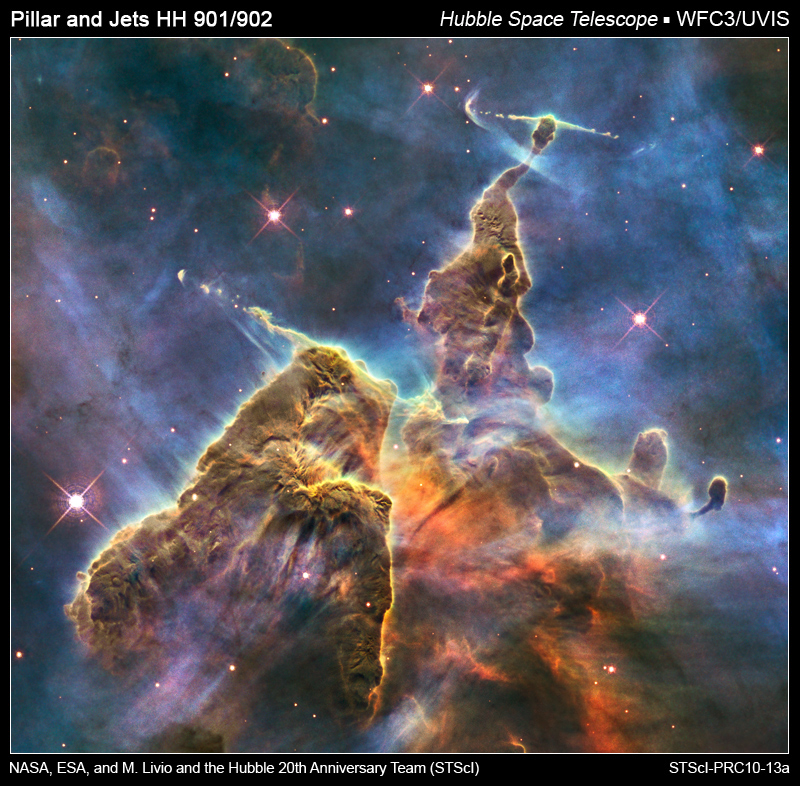
\includegraphics[width=0.6\textwidth]{carina}
    \end{figure}
 \column{0.45\textwidth} 
 \textbf{Carina Nebula:} Largest-seen star-birth regions in the galaxy
 \end{columns}

\begin{block}{\small Observation and expectation from Standard Cosmological Model (SCM):}
\begin{center}
\renewcommand*{\arraystretch}{1.3}\small
\begin{tabular}{l |l|l}
                       & $\eta = \displaystyle (n_b - n_{\bar{b}})/n_\gamma$ & \\\hline
 Observation              & $\left( 6.11^{+ 0.3}_{-0.2} \right) \times \num{e-10} $      &  Best Fit Cosmological Model\,\textcolor{PineGreen}{\cite{Bennett:2003bz}}\\
                       & $(5.53-6.76) \times \num{e-10}$ & WMAP\,\textcolor{PineGreen}{\cite{Barger:2003zg}} \\
 Expectation from SCM  & $\sim \num{e-18}$ & Bernreuther (2002)\,\textcolor{PineGreen}{\cite{Bernreuther:2002uj}}\\
\end{tabular}
\end{center}
\end{block}


\begin{alertblock}{}
 \begin{itemize}
 \item SCM gets it wrong by more than 8 orders of magnitude. 
\end{itemize}
\end{alertblock}

\end{frame}
\begin{frame}
\frametitle{Electric dipole moments (EDMs)}

\begin{columns}
\column{0.72\textwidth}
\vspace{-0.4cm}
 \begin{block}{For particles with EDM $\vec d$ and MDM $\vec \mu$ ($\propto \vec s $),}
 \begin{itemize}
     \item non-relativistic Hamiltonian:
        \begin{equation}
            H = -\vec \mu \cdot \vec B - \vec d \cdot \vec E \nonumber
        \end{equation}
 \item \textbf{Energy of magnetic dipole} invariant under $P$ and $T$:
 \begin{equation}
  -\vec \mu \cdot \vec B \overbrace{\longrightarrow}^{P \text{ or } T} -\vec \mu \cdot \vec B \nonumber
 \end{equation}
 No other direction than spin  $\Rightarrow$ $\vec d$ parallel to $\vec \mu$ ($\vec s$). 
  \item \textbf{Energy of electric dipole} $H = - \vec d \cdot \vec E$, includes term 
  \vspace{-0.2cm}
  \begin{equation}
  \vec s \cdot \vec E \overbrace{\longrightarrow}^{P \text{ or } T} - \vec s \cdot \vec E,
 \end{equation}
 % \end{itemize}
 \end{itemize}
 \end{block}
\column{0.27\textwidth}
\begin{figure}
	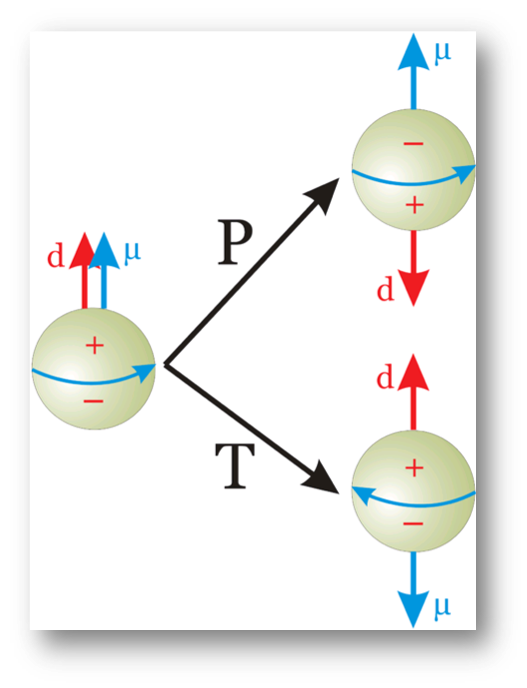
\includegraphics[width=1\textwidth]{EDM-graphic}
\end{figure}
\end{columns}
 

\begin{alertblock}{\textbf{EDMs violate both $P$ and $T$ symmetry}}
\begin{itemize}   
     \item EDMs possibly constitute the missing cornerstone to explain surplus of matter over antimatter in the Universe.
     \begin{itemize}
        \item Non-vanishing EDMs would add \nth{4} quantum number to fundamental particles (besides $m$, $q$, and $s$).  
     \end{itemize}
\end{itemize}
\end{alertblock}


%  \column{0.3\textwidth}
% \vspace{-0.2cm}
%     \begin{figure}
%       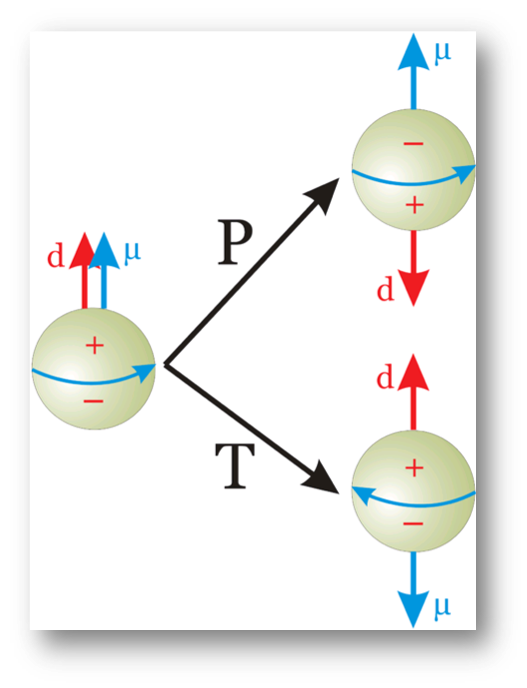
\includegraphics[width=1\textwidth]{EDM-graphic}
%     \end{figure}
% % \end{columns}

\end{frame}
\begin{frame}
\frametitle{Naive estimate of scale of nucleon EDM}

\vspace{-0.5cm}
\begin{block}{From Khriplovich \& Lamoreux \textcolor{PineGreen}{\cite{Khriplovich:1997ga}} and Nikolaev \textcolor{PineGreen}{\cite{Rathmann:2013rqa}}:}
%	\vspace{-0.2cm}
\begin{itemize}
  \item $CP$ and $P$ conserving magnetic moment $\approx$ nuclear magneton $\mu_N$.
  \begin{equation}
     \mu_N = \frac{e}{2m_p} \sim \SI{e-14}{e.cm}. \nonumber
  \end{equation}
  \vspace{-0.4cm}
  \item A non-zero EDM requires:
  \begin{itemize}
   \item $P$ violation: price to pay is $\approx \SI{e-7}{}$, and
   \item $CP$ violation (from $K$ decays): price to pay is $\sim \SI{e-3}{}$.
  \end{itemize}
  \item In summary: 
  \begin{equation}
   \textcolor{red}{\boxed{|d_N| \sim \num{e-7} \times \num{e-3} \times \mu_N \sim \SI{e-24}{e.cm}}}\nonumber
  \end{equation}
  \item In Standard model (without $\theta_\text{QCD}$ term):    
    \begin{equation}
      \textcolor{red}{\boxed{|d_N| \sim \num{e-7} \times \SI{e-24}{e.cm}  \sim \SI{e-31}{e.cm}}}   \nonumber  
    \end{equation}
 \end{itemize}
\end{block}

\vspace{-0.3cm}
\begin{alertblock}{Region to search for Beyond Standard Model (BSM) physics  }
%\vspace{-0.2cm}	
\begin{itemize}
 \item from nucleon EDMs with $\theta_\text{QCD}=0$:
\end{itemize}
 \centering $\boxed{\SI{e-24}{e.cm} > |d_N| > \SI{e-31}{e.cm}}$.
\end{alertblock}

\end{frame}

\begin{frame}
\frametitle{Motivation}
\framesubtitle{}

\vspace{-0.2cm}
\begin{block}{Issues we are addressing}
	\begin{itemize}
		\item Matter over antimatter dominance / Baryon asymmetry in the Universe
		\item \textcolor{red}{Nature of Dark Matter (DM)}
	\end{itemize}
\end{block}

\vspace{-0.2cm}
\begin{block}{Experimental approach}
	\begin{itemize}
		\item Measure of static Electric Dipole Moments (EDM) of fundamental particles
		\item \textcolor{red}{Search for axion-like particles as DM candidates through oscillating EDMs}
	\end{itemize}
\end{block}

\vspace{-0.2cm}
\begin{center}
	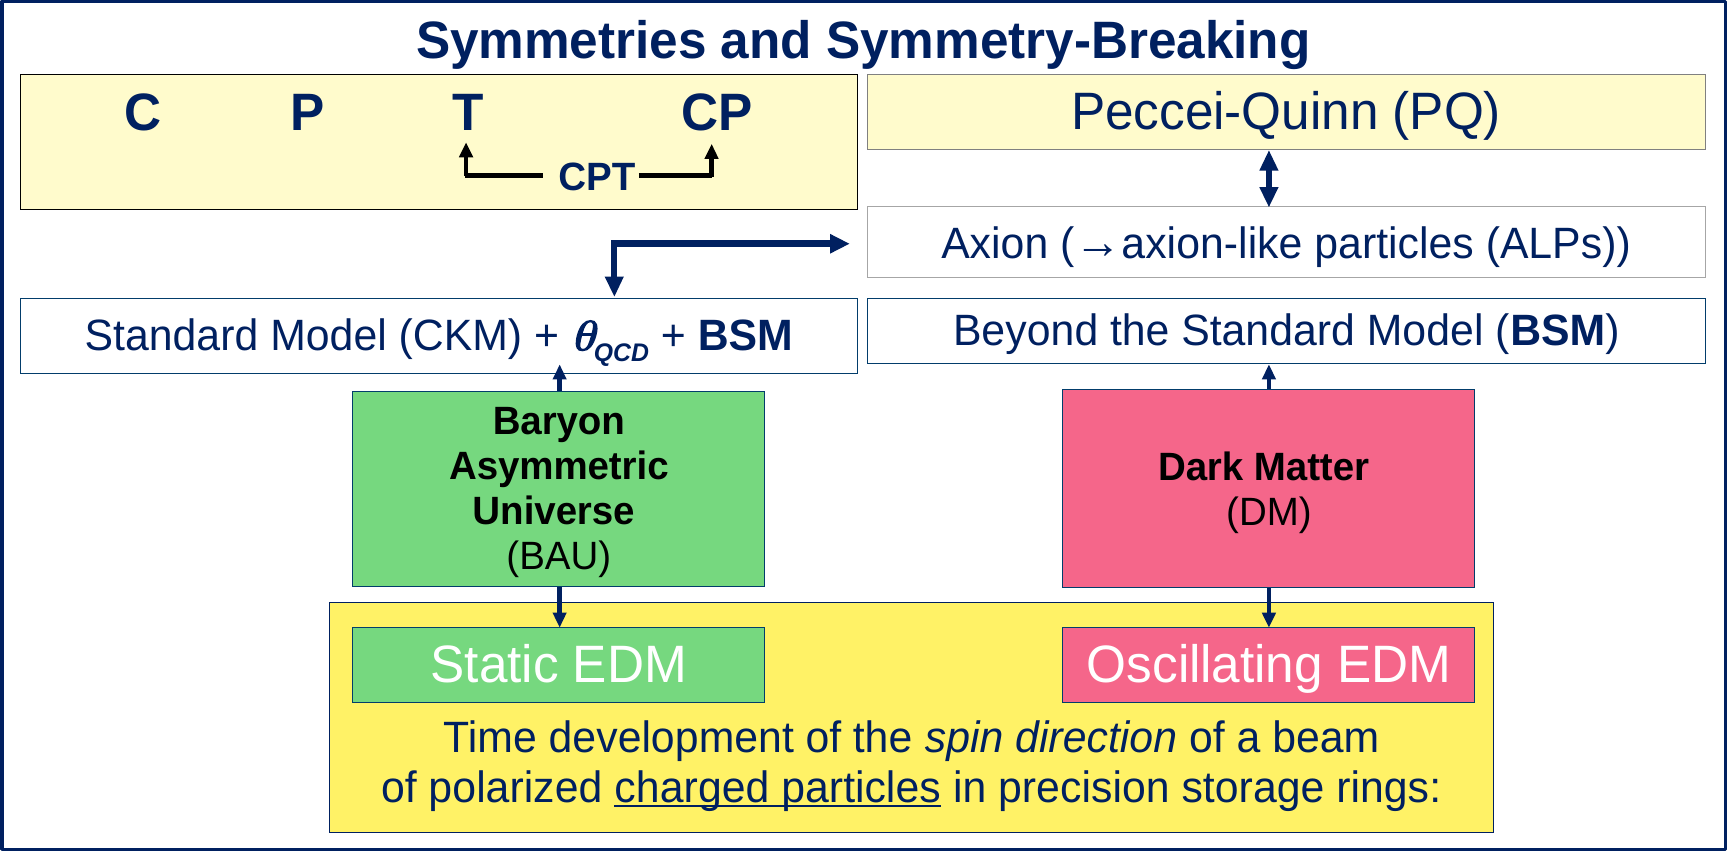
\includegraphics[height=0.45\textheight]{Fig3new.png}
\end{center}

\end{frame}
%--------------------------------------------------------
%--------------------------------------------------------
\begin{frame}
\frametitle{Status of static EDM searches\,\textcolor{PineGreen}{\cite[\textcolor{orange}{CYR '21}]{CPEDM:2019nwp}}}

\vspace{-0.5cm}
\begin{figure}
      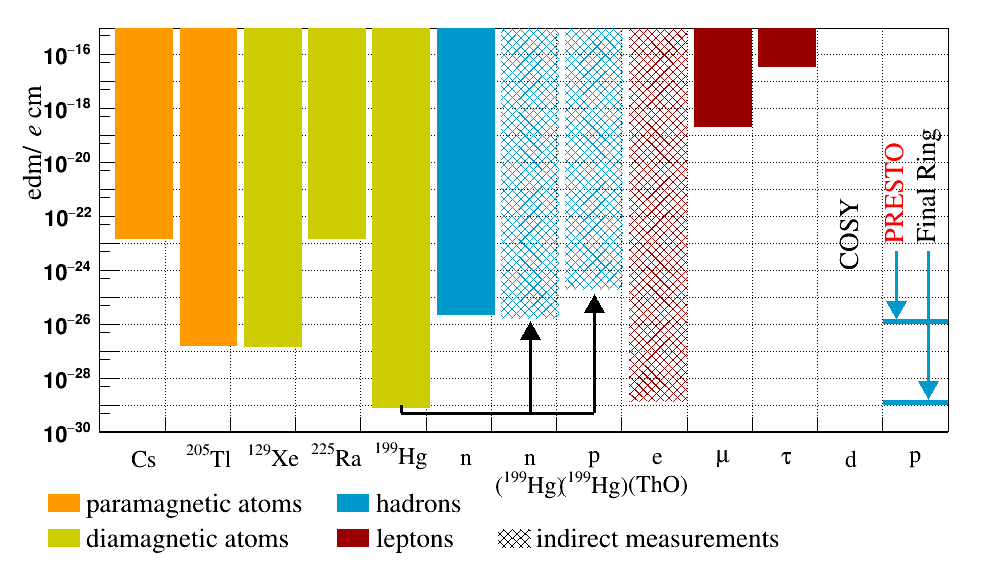
\includegraphics[width=0.6\textwidth]{Figure_EDM_Bounds.png}
\end{figure}
    
\vspace{-0.3cm}    
\begin{block}{Missing are \textit{direct} EDM measurements:}
\begin{itemize}
 \item  No direct measurements of electron: limit obtained from (ThO molecule).
 \item  No direct measurements of proton: limit obtained from  $\Hg{199}$.
 \item \textbf{No measurement yet of deuteron EDM.}
\end{itemize}
\end{block}

\vspace{-0.2cm}
\begin{alertblock}{Theory stresses that}
\centering \textbf{EDM of single particle not sufficient to identify $CP$ violating source}\,\textcolor{PineGreen}{\cite{Bsaisou:2015:1}}
\end{alertblock}
\end{frame}
%--------------------------------------------------------
\begin{frame}
\frametitle{Axion Dark Matter search with Storage Ring EDM method  }



\begin{figure}
		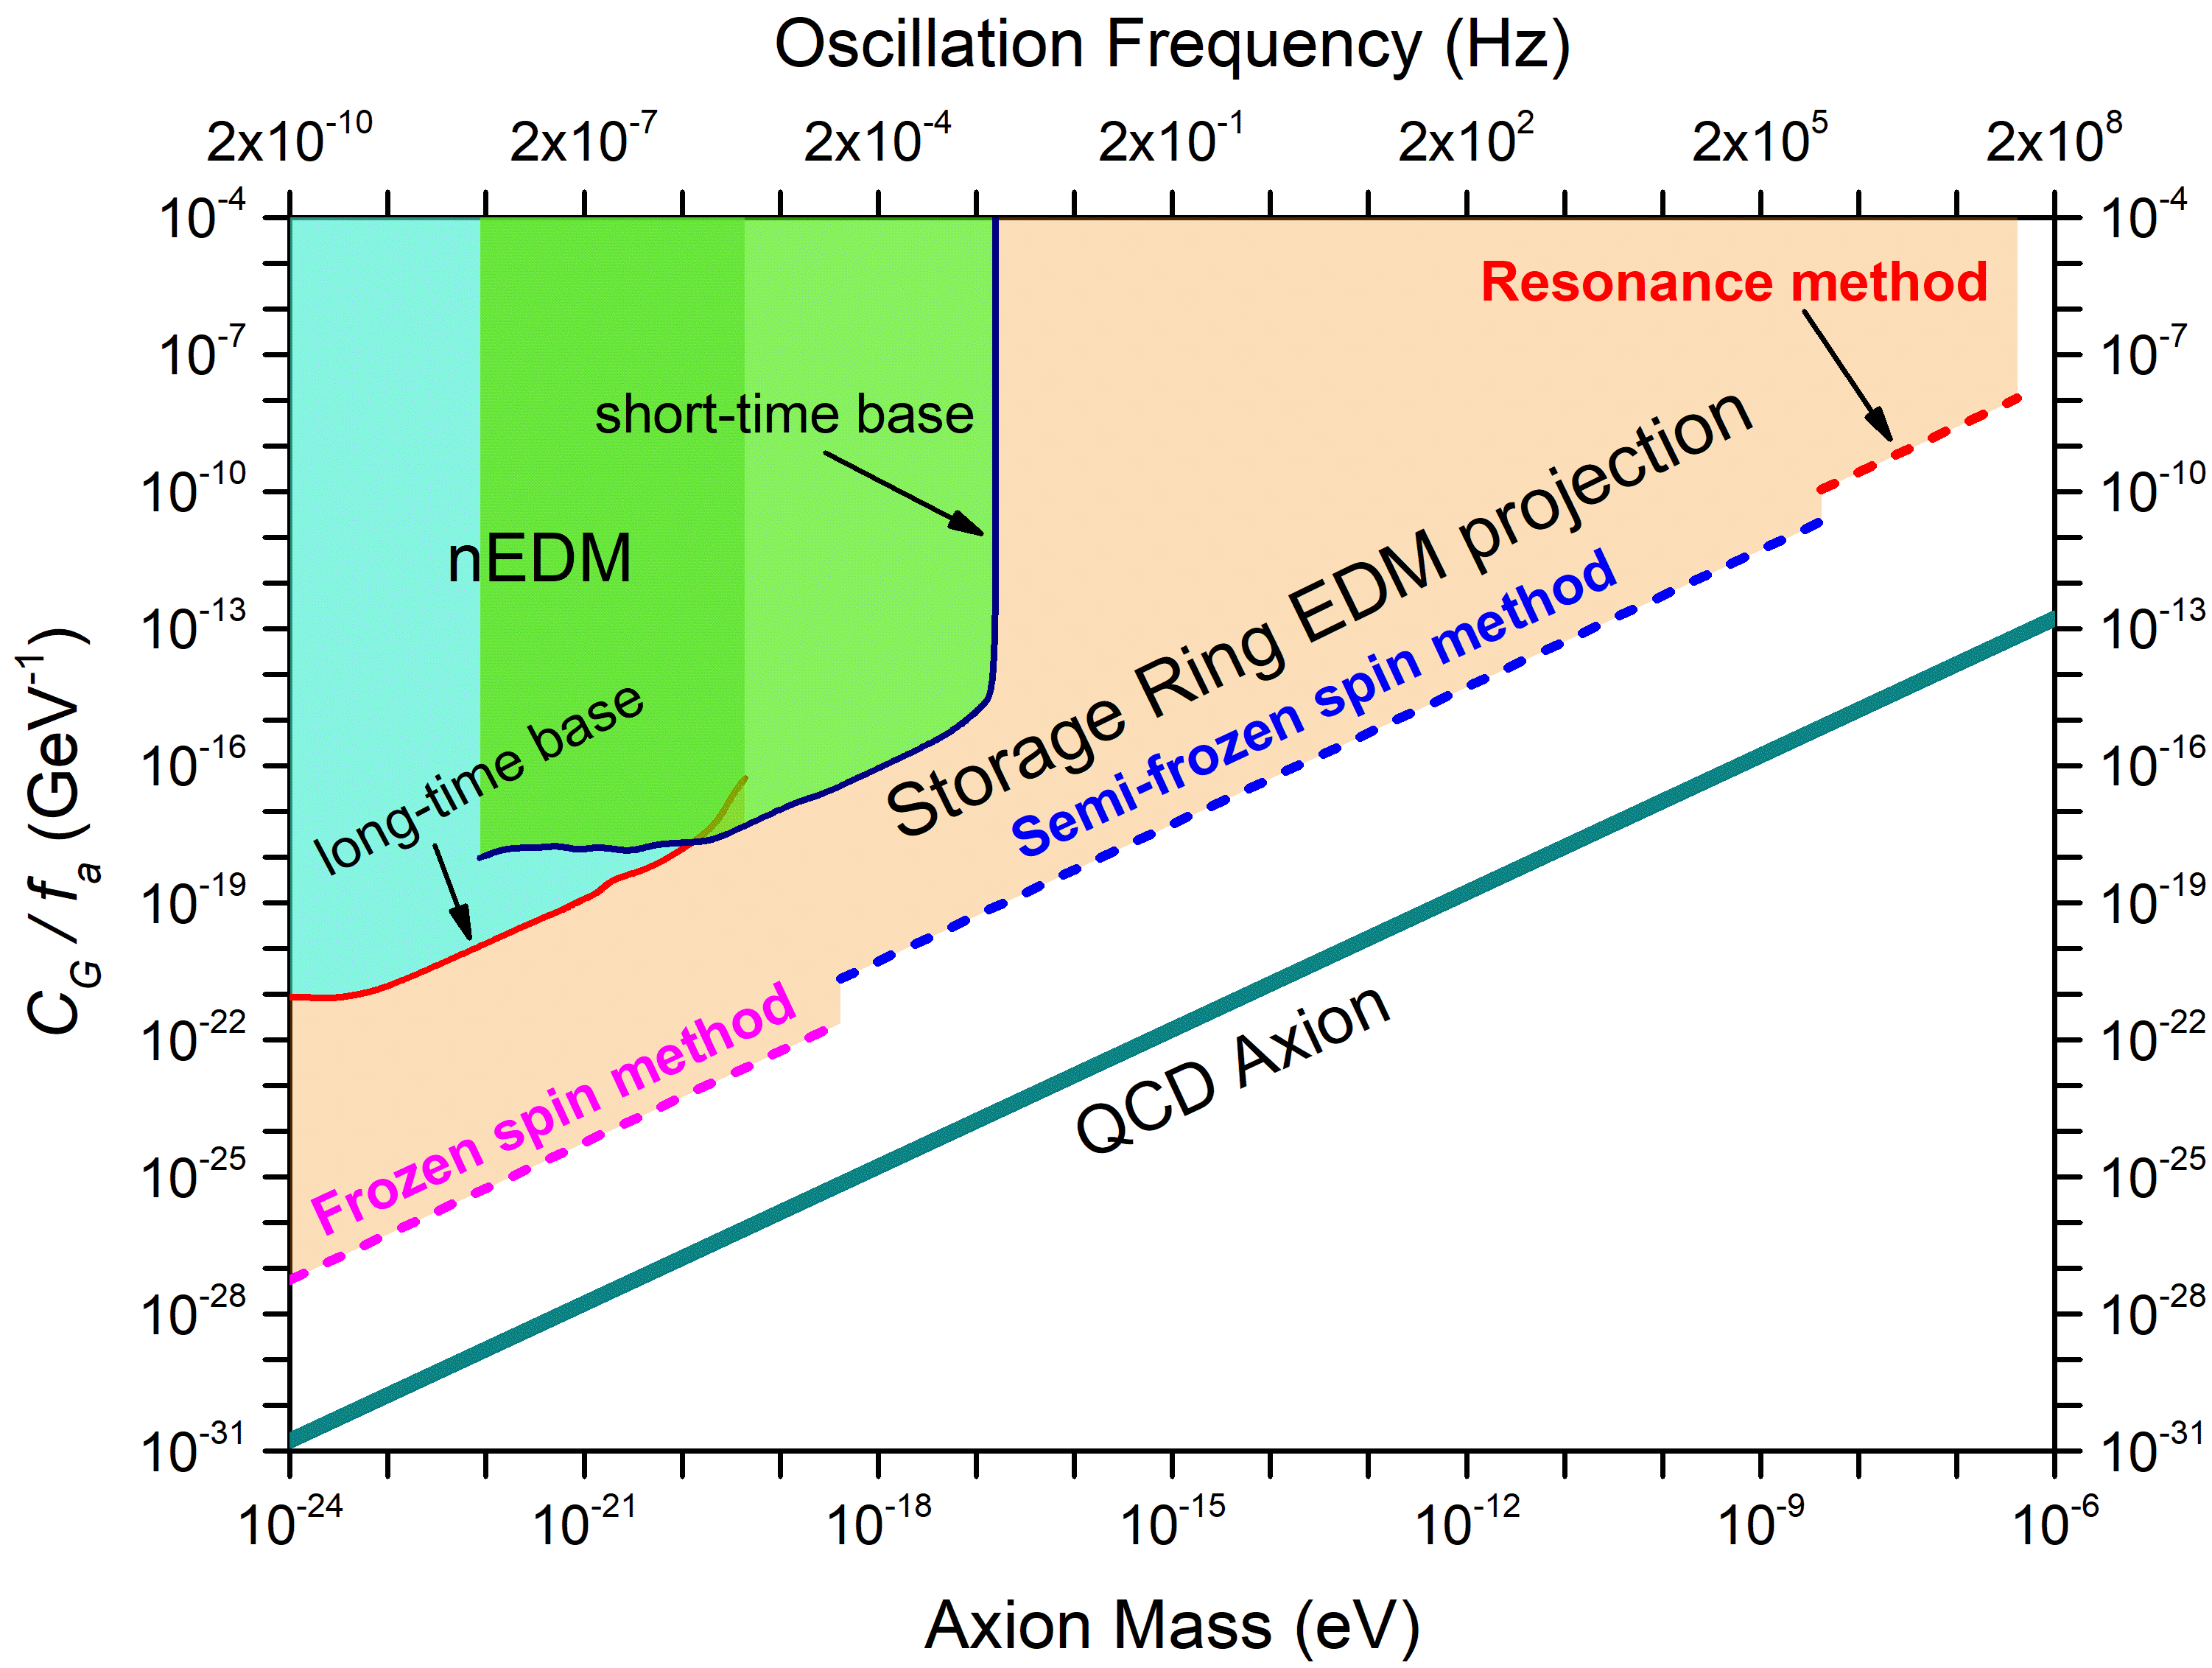
\includegraphics[width=0.7\textwidth]{limit.png}
		\caption{Experimental limits for axion-gluon coupled oscillating EDM measurements (from\,\textcolor{PineGreen}{\cite{Chang:2017ruk}}).}
\end{figure}





\end{frame}

\section{Measurement principles \& experimental techniques}
\begin{frame}
\frametitle{Measurement of  EDM in storage ring}
\framesubtitle{\textbf{\textbf{Protons at magic momentum in pure electric ring}}}


\vspace{-0.2cm}
\begin{block}{How to measure EDM of proton:}
	\begin{enumerate}
		\item Place polarized particles in a storage ring.
		\item Align spin along direction of flight at magic momentum. 
		\begin{itemize}
			\item[$\Rightarrow$] \textit{freeze} horizontal spin precession.
		\end{itemize}
		\item Search for time development of vertical polarization. 
	\end{enumerate}
\end{block}

\begin{columns}
	\column{0.35\textwidth}
	\hspace{0.3cm}
	\begin{tikzpicture}
	\node[anchor=south west,inner sep=0] (image) at (0,0) {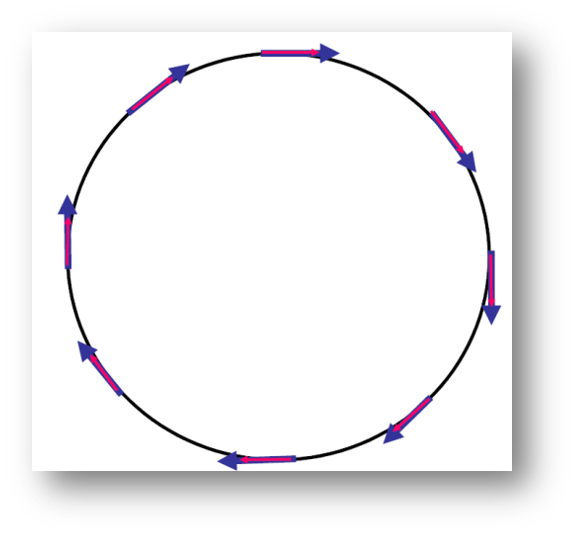
\includegraphics[width=0.8\textwidth]{frozen-spin.png}};
	\begin{scope}[x={(image.south east)},y={(image.north west)}]
	\draw (0.5,0.7)  node[font=\large] {$\vec \Omega = 0$};
	\draw (0.5,0.45)  node[font=\large] {$\displaystyle\frac{\dd \vec S}{\dd t} = \vec d \times \vec E$};
	\end{scope}
	\end{tikzpicture}
	\column{0.6\textwidth}
	\vspace{-0.3cm}
	\begin{figure}
		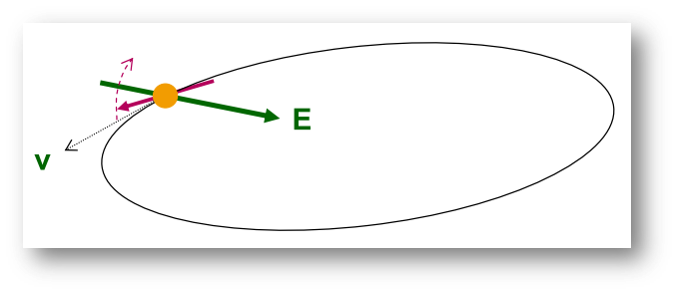
\includegraphics[width=1\textwidth]{polarization-buildup.png}
	\end{figure}
\end{columns}

\vspace{-0.3cm}
\begin{alertblock}{Storage ring method to measure EDMs of charged particles:}
	\begin{itemize}
		\item \textbf{Magic rings with spin frozen} along  momentum of particle.
		\item Polarization buildup $p_y(t)\propto d$.
	\end{itemize}
\end{alertblock}

\end{frame}

\begin{frame}
\frametitle{Spin precession of particles with MDM and EDM}
\framesubtitle{}

\vspace{-0.5cm}
\begin{block}{In rest frame of particle}
	\begin{itemize}
		\item Equation of motion for spin vector $\vec S$:
		\begin{equation}
			\frac{\dd \vec S}{\dd t} = \vec \Omega \times \vec S = \vec \mu \times \vec B + \vec d \times \vec E.
		\end{equation}
	\end{itemize}
\end{block}


\begin{block}{With protons in a ring}
	\begin{figure}
		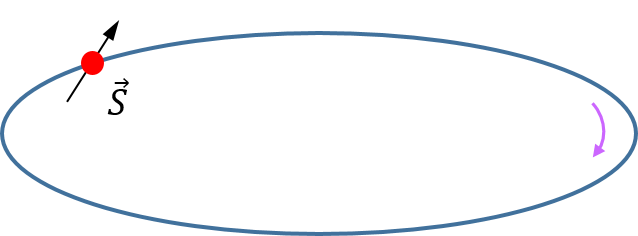
\includegraphics[width=0.6\textwidth]{proton-orbit}
	\end{figure}
	\begin{itemize}
		\item[$\rightarrow$] Spin-precession with MDMs and EDMs described by Thomas-BMT Eq.\,\textcolor{PineGreen}{\cite{Fukuyama:2013ioa}}.
	\end{itemize}
\end{block}

\end{frame}

\begin{frame}
\frametitle{Frozen-spin}
\framesubtitle{}

\vspace{-0.3cm}
\begin{block}{Spin-precession of particle MDM   \textit{relative} to direction of flight:}
	\begin{equation}
	\begin{split}
	\vec \Omega & = \vec \Omega_\text{MDM} - \vec \Omega_\text{cyc} \\
	& = - \frac{q}{\gamma m} \left[G \gamma \vec B_\perp + (1 + G) \vec B_\parallel - \left(G\gamma - \frac{\gamma}{\gamma^2 -1} \right) \frac{\vec \beta \times \vec E}{c}\right].  
	\end{split}
	\end{equation}
	\vspace{-0.3cm}
	\begin{itemize}
		\item[$\Rightarrow$] \textbf{$\vec \Omega = 0$ called \textit{frozen spin}, because  momentum and spin stay aligned.}
	\end{itemize}
	\begin{itemize}
		\item In the absence of magnetic fields ($B_\perp = \vec B_\parallel = 0$), 
		\begin{equation}
		\vec \Omega=0, \text{ if } \left(G\gamma - \frac{\gamma}{\gamma^2 -1} \right) = 0.
		\label{eq:magic-momentum}
		\end{equation}
		\vspace{-0.3cm}
		\begin{itemize}
			\item[-] Possible for particles with $G>0$:   proton ($G=1.793$) or electron ($G=0.001$).
		\end{itemize}
	\end{itemize}
\end{block}


\begin{exampleblock}{For protons:  (\ref{eq:magic-momentum}) $\Rightarrow$ \textit{magic momentum}:}
	\begin{equation}
	G- \frac{1}{\gamma^2-1} = 0 \Leftrightarrow G = \frac{m^2}{p^2} 
	\quad \Rightarrow \quad \boxed{p = \frac{m}{\sqrt{G}} = \SI{700.740}{MeV.c^{-1}}}
	\end{equation}
\end{exampleblock}

\end{frame}
\begin{frame}
\frametitle{Measurement of EDM in a magnetic ring}
\framesubtitle{\textbf{First-ever direct EDM measurement using this method}}

\vspace{-0.4cm}
\begin{block}{In magnetic ring}
	\begin{itemize}
		\item When external electric fields  in ring vanish, $\vec E = 0$,  spin motion  governed by  radial field $\vec E = c\vec \beta \times \vec B $, induced by  relativistic motion in  vertical $\vec B$ field:
		\vspace{-0.1cm}
		\begin{equation}
			\frac{\dd \vec S}{\dd t} \propto \vec d \times \vec E \,\,\,\, \text{(see \textcolor{PineGreen}{\small \cite{PhysRevAccelBeams.23.024601}})}
		\end{equation}
		\vspace{-0.3cm}
		 \begin{itemize}
			\item[$\rightarrow$] only small oscillation of vertical component $p_y$ due to EDM.
		 \end{itemize} 
		\item \textcolor{Maroon}{\textbf{Use RF Wien filter to accumulate EDM signal}}\,\textcolor{PineGreen}{\small \cite{Slim2016116, PhysRevAccelBeams.23.024601}}:
		\begin{itemize}
			\item[$+$] Long spin-coherence time $>\SI{1000}{s}$\,\textcolor{PineGreen}{\small\cite{PhysRevLett.117.054801}}
			\item[+] Spin tune determination $\Delta\nu_s/\nu_s\approx \num{e-10}$\,\textcolor{PineGreen}{\small \cite{PhysRevLett.115.094801}} $\rightarrow$ tune RF Wien filter frequency
			\item[+] Phase-lock of spin phase relative to  Wien filter RF\,\textcolor{PineGreen}{\small \cite{PhysRevLett.119.014801}}.
			\item[+] Two-bunch method: pilot and signal bunch \textcolor{PineGreen}{\small \cite{Slim:2023lpd,Nikolaev:2023srx}}
			\begin{itemize}
				\item[-] pilot bunch shielded from Wien filter RF by fast RF switches 
				\item[-] pilot bunch $\rightarrow$ unperturbed spin precession $\rightarrow$ RF Wien filter on resonance
				\item[-] observe $p_y$ oscillations over many periods    
				\item[-] \textcolor{Maroon}{\textbf{pilot bunch $\rightarrow$ co-magnetometry}}
			\end{itemize}
			
		\end{itemize}
	\end{itemize} 
\end{block}

\vspace{-0.3cm}
\begin{exampleblock}{Accumulated knowledge compiled in}
	\hspace{1cm}	\textcolor{orange}{\textbf{2021 CERN Yellow Report}}\,\textcolor{PineGreen}{\small \cite{CPEDM:2019nwp}}
\end{exampleblock}

\end{frame}

\section{Achievements}
\subsection{Spin-tune determination}
\begin{frame}
\frametitle{Principle of spin-coherence time measurement}
\framesubtitle{}

\begin{figure}
              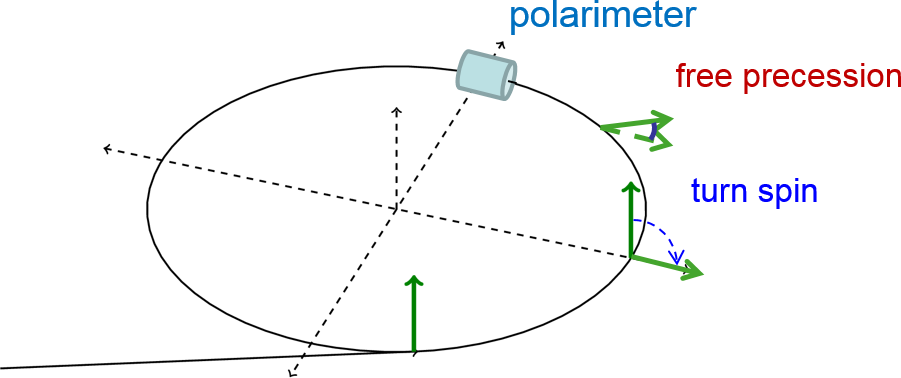
\includegraphics[height=0.27\textheight]{SCT-setup.png}
              \hspace{0.4cm}
			 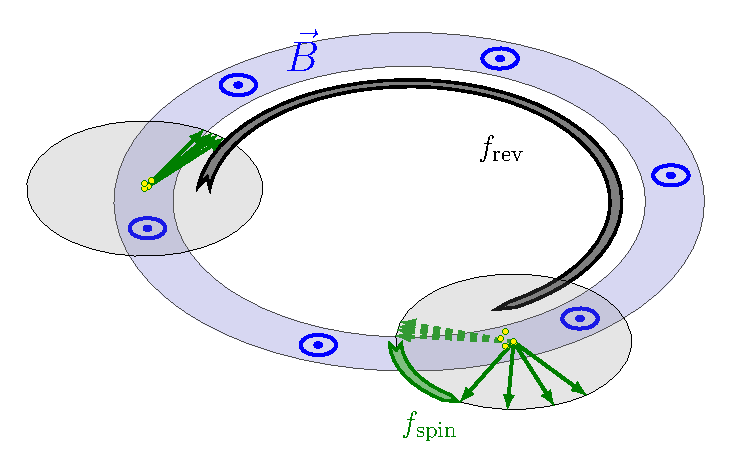
\includegraphics[height=0.29\textheight]{spintune.pdf}
\end{figure}

\begin{block}{Measurement procedure:}
\begin{enumerate}
 \item Vertically polarized deuterons stored at $p \simeq \SI{1}{GeV.c^{-1}}$.
 \item Polarization flipped into horizontal plane with RF solenoid ($\approx \SI{200}{ms}$). 
 \item Beam extracted on Carbon target with ramped bump or by heating.
 \item Horizontal (in-plane) polarization determined from $U-D$ asymmetry.
\end{enumerate}
\end{block}

\end{frame}
\begin{frame}
\frametitle{Detector system: EDDA\,\textcolor{PineGreen}{\cite{Albers:2004iw}}}
\framesubtitle{}
 
 \vspace{-0.6cm}
\begin{columns}[c]
 \column{0.5\textwidth}
 \begin{figure}
     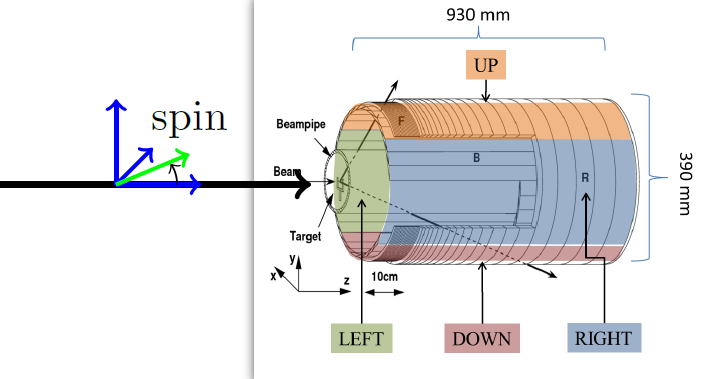
\includegraphics[height=3.5cm]{EDDA.png}
 \end{figure}
 \column{0.35\textwidth}
 \begin{figure}
     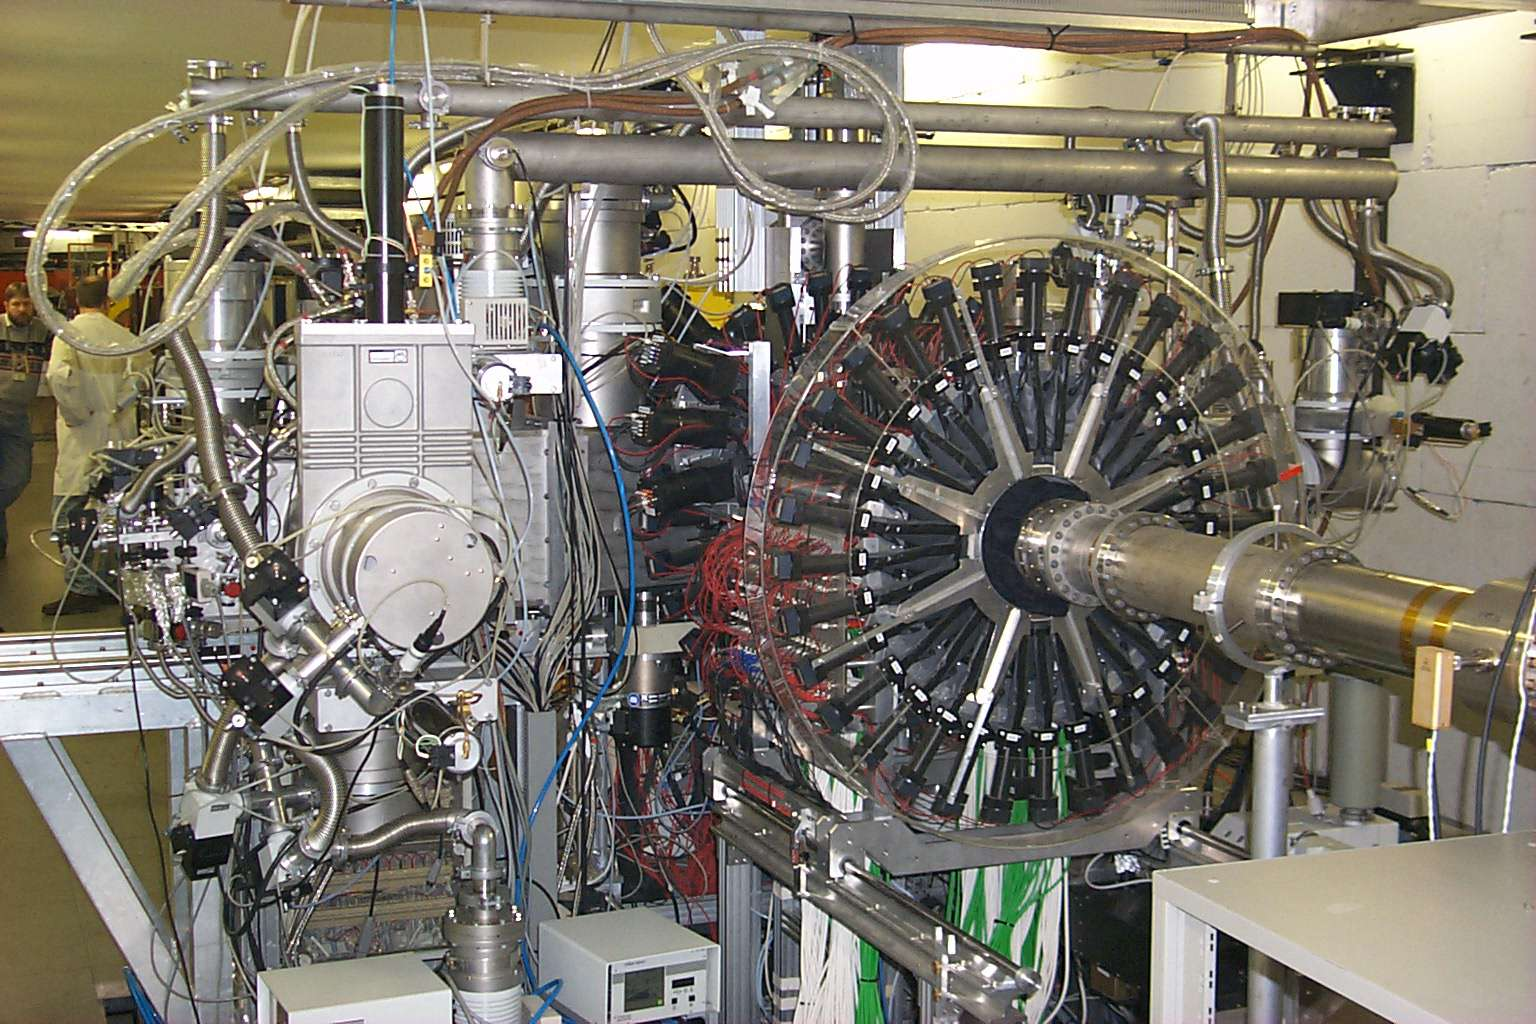
\includegraphics[height=2.5cm]{EDDA-Foto.png} 
 \end{figure}
\end{columns}

\vspace{-0.2cm}
\begin{block}{EDDA  used to determine $\vec p \vec p$ elastic polarization observables:}
\begin{itemize}
 \item Deuterons at $p = \SI{1}{GeV.c^{-1}}$, $\gamma = 1.13$, and $\nu_s = \gamma G \simeq -0.161$
 \item Spin-dependent differential cross section on unpolarized target:
\begin{equation}
    N_\text{U,D} \propto 1 \pm \frac{3}{2} p_x A_y \sin(\underbrace{\nu_s \cdot f_\text{rev}}_{f_s = \SI{-120.7}{kHz}}\cdot t), \text{ where } f_\text{rev} = \SI{750.0}{kHz}.
\end{equation}
\end{itemize}
\end{block}

\vspace{-0.3cm}
\begin{alertblock}{JEPO polarimeter}
	Lateron, EDDA replaced by dedicated new polarimeter, based on LYSO crystals.
\end{alertblock}
 
\end{frame}
\subsection{Spin-coherence time improvement}
\begin{frame}
\frametitle{Spin coherence time}
\framesubtitle{Most polarization experiments unaffected by coherence of spins along $\vec n_\text{co}$}

\vspace{-0.7cm}
\begin{columns}[t]
	\column{0.48\textwidth}
	\begin{exampleblock}{\normalsize \textbf{Spins aligned:}}
		\centering\small Ensemble \textit{coherent}
	\end{exampleblock}
	\vspace{-0.3cm}
	\begin{figure}
		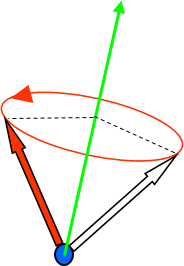
\includegraphics[height=1.5cm]{SCT-1.png}
	\end{figure}
	\column{0.48\textwidth}
	\begin{exampleblock}{\normalsize \textbf{Spin vectors out of phase:} }
		\centering\small Ensemble \textit{decoherent}
	\end{exampleblock}
	\vspace{-0.45cm}
	\begin{figure}
		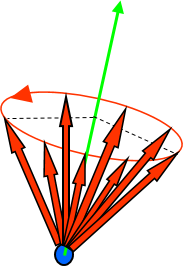
\includegraphics[height=1.5cm]{SCT-2.png}
	\end{figure}
\end{columns}
\begin{center}
	\small  \textbf{$\Rightarrow$ Polarization along $\vec n_\text{co}$ not affected}
\end{center}

\vspace{-0.5cm}
\begin{columns}[]
	\column{0.48\textwidth}
	\begin{exampleblock}{\normalsize \textbf{With frozen spins:} $\vec S \perp  \vec n_\text{co}$:}
		\centering\small Spins aligned
	\end{exampleblock}
	\vspace{-0.3cm}
	\begin{figure}
		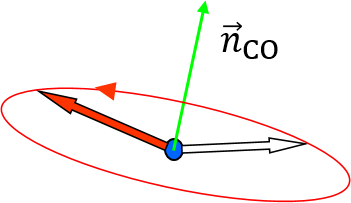
\includegraphics[height=1.1cm]{SCT-3.png}
	\end{figure}
	\column{0.48\textwidth}
	\begin{exampleblock}{\normalsize \textbf{With time:}}
		\centering\small Spins out of phase in horizontal plane
	\end{exampleblock}
	\vspace{-0.3cm}
	\begin{figure}
		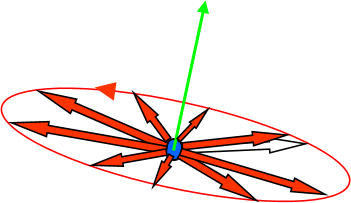
\includegraphics[height=1.1cm]{SCT-4.png}
	\end{figure}
\end{columns}
\begin{center}
	\small  \textbf{$\Rightarrow$ In-plane polarization vanishes}
\end{center}

\vspace{-0.5cm}
\begin{alertblock}{In machines with frozen spins:}
	\centering\textbf{ Buildup time $t$ to observe polarization $p_y(t)$ is limited by $\tau_\text{SCT}$.}
\end{alertblock}

\end{frame}
\begin{frame}
\frametitle{Optimization of spin-coherence time \textcolor{PineGreen}{\cite{PhysRevLett.117.054801}}}
\framesubtitle{}

Precise adjustments of three sextupole families in the ring

\begin{columns}[]
	\column{0.53\textwidth}
	\begin{figure}
		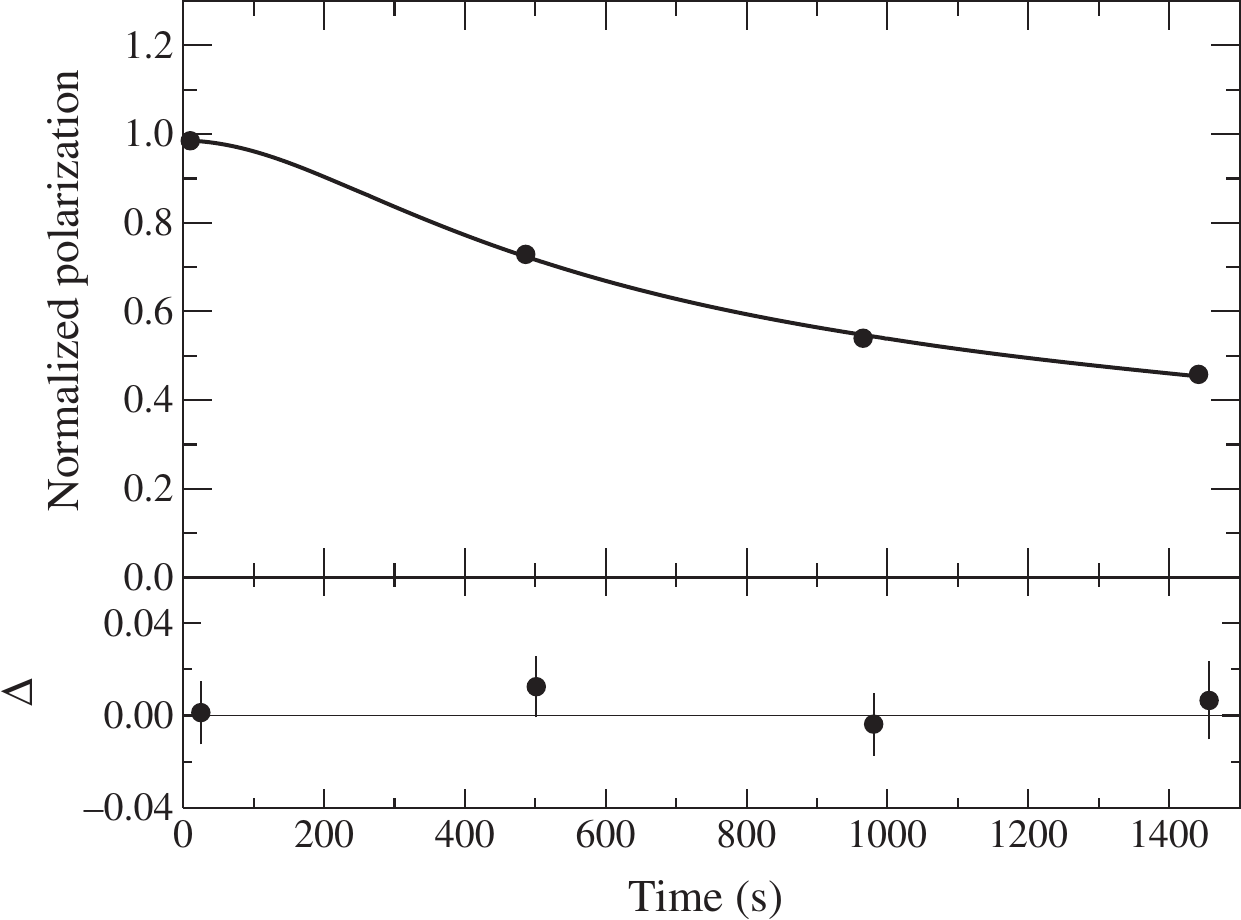
\includegraphics[width=0.95\textwidth]{spin-coherence-time-from-PRL.png}
	\end{figure}
	\column{0.4\textwidth}
	\begin{block}{JEDI progress on $\tau_\text{SCT}$:}
		\begin{equation}
		\textcolor{red}{\mathbf{\tau_\text{SCT} = (782 \pm 117)\,\text{s}}} \nonumber
		\end{equation}
		\vspace{-0.5cm}
		\begin{itemize}
			\item Previous record: $\tau_\text{SCT}(\text{VEPP}) \approx \SI{0.5}{s}$\,\textcolor{PineGreen}{\cite{Vasserman1987302}} ($\approx \num{e7}$ spin revolutions).
		\end{itemize}
	\end{block}
\end{columns}

\begin{alertblock}{\textbf{Spring 2015:} Way beyond anybody’s expectation:}
	\begin{itemize}
		\item With about $\num{e9}$ stored deuterons.
		\item Long spin coherence time was one of main obstacles of srEDM experiments.
		\item Large value of $\tau_\text{SCT}$ of crucial importance (\ref{eq:statistical-error-EDM-experiment}), since $ \sigma_\text{stat} \propto {\tau_\text{SCT}}^{-1}$.
	\end{itemize}
\end{alertblock}

\end{frame}

\begin{frame}
\frametitle{Precision determination of spin tune\,\textcolor{PineGreen}{\cite{PhysRevLett.115.094801}} I}

\begin{block}{Time-stamping events in each detector quadrant accurately:}
\begin{enumerate}
	\item Based on turn number $n$, \SI{100}{s} measurement interval split into turn intervals of $\Delta n = \SI{e6}{turns}$, each interval lasting $\approx \SI{1.3}{\second}$.
	\item  For all events, spin phase advance $\varphi_s = 2 \pi | \nu_s^\text{fix} |n $ calculated assuming certain fixed spin tune $\nu_s^\text{fix}$.
	\item Either map events into one full polarization oscillation in range $\varphi_s \in [0, 2\pi)$, or perform Fourier analysis of rates in detector $\Rightarrow$ determine  $\tilde \varepsilon$ and $\tilde \phi$ in 
	\begin{equation}
	\varepsilon(\varphi_s) = \tilde \varepsilon \sin(\varphi_s + \tilde \varphi)\,.
	\end{equation}
\end{enumerate}
\end{block}

\vspace{0.3cm}
\begin{columns}
	\column{0.45\textwidth}
	\centering 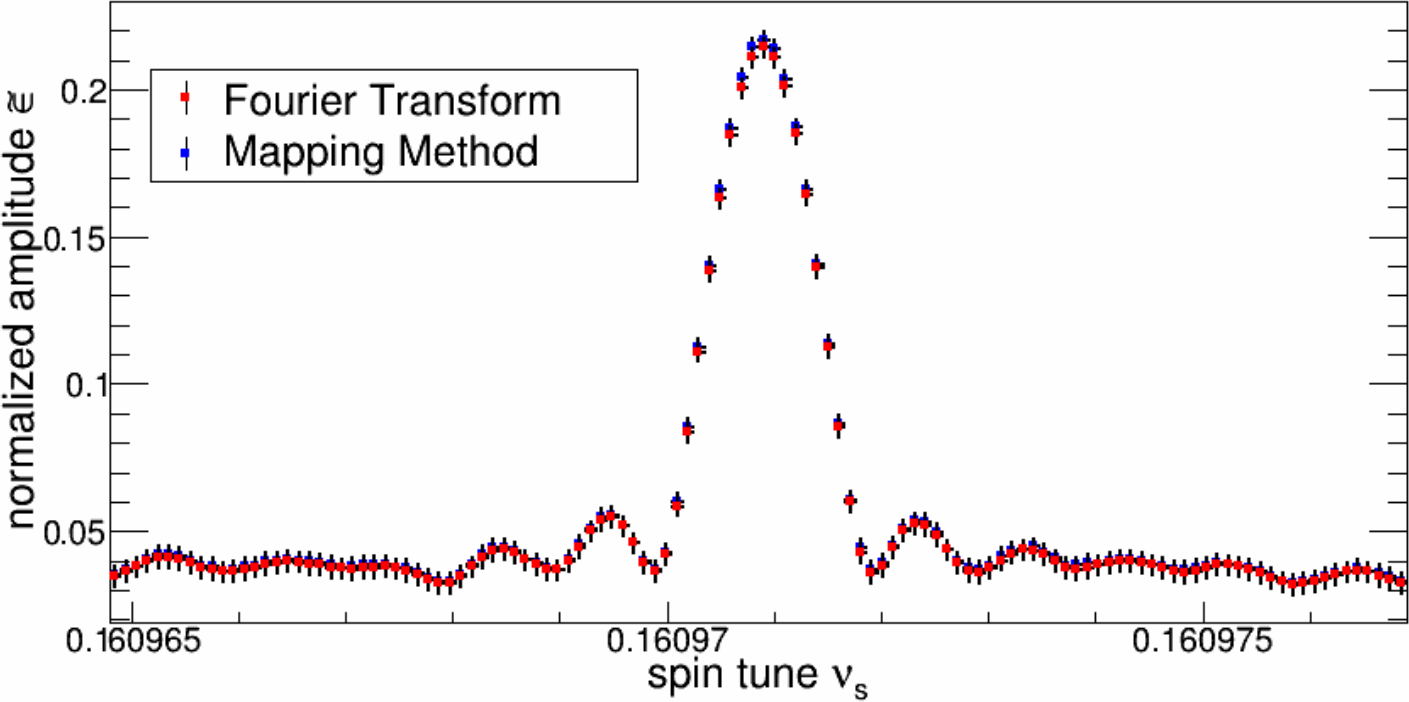
\includegraphics[height = 0.3\textheight]{spin-tune-spectrum.png} 
	\column{0.45\textwidth}  
	\centering 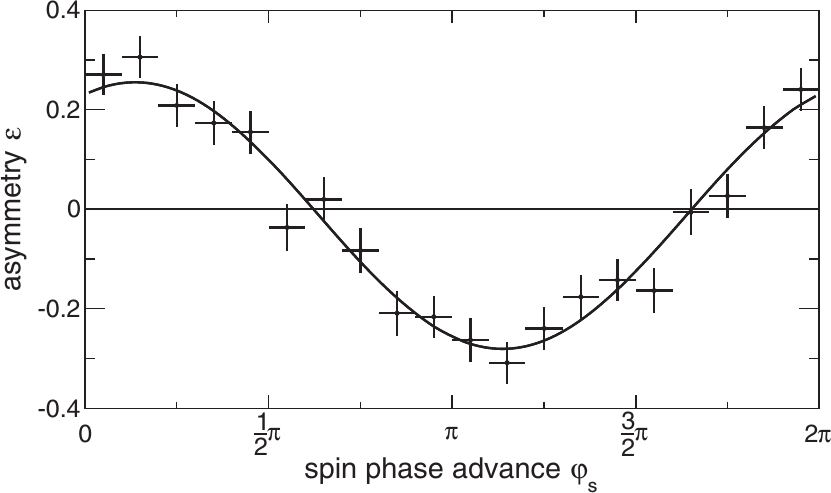
\includegraphics[height = 0.3\textheight]{phase-plot-spin-tune.png}
\end{columns}

\end{frame}
\begin{frame}
\frametitle{Precision determination of the spin tune\,\textcolor{PineGreen}{\cite{PhysRevLett.115.094801}} II}

\vspace{-0.3cm}
\begin{columns}[c]
\column{0.46\textwidth}
\begin{block}{Precise time-stamping of events,}
\begin{itemize}
 \item allows us to monitor phase of measured asymmetry with (assumed) fixed spin tune $\nu_s$ in a $\SI{100}{s}$ cycle:
 \begin{equation}
 \begin{split}
    \nu_s(n) & = \nu_s^\text{fix} + \frac{1}{2\pi} \frac{\dd \tilde{\phi}}{\dd n}\\
             & = \nu_s^\text{fix} + \Delta \nu_s(n)
 \end{split}
 \end{equation}
\end{itemize}
\end{block}

\column{0.5\textwidth}
\begin{figure}
    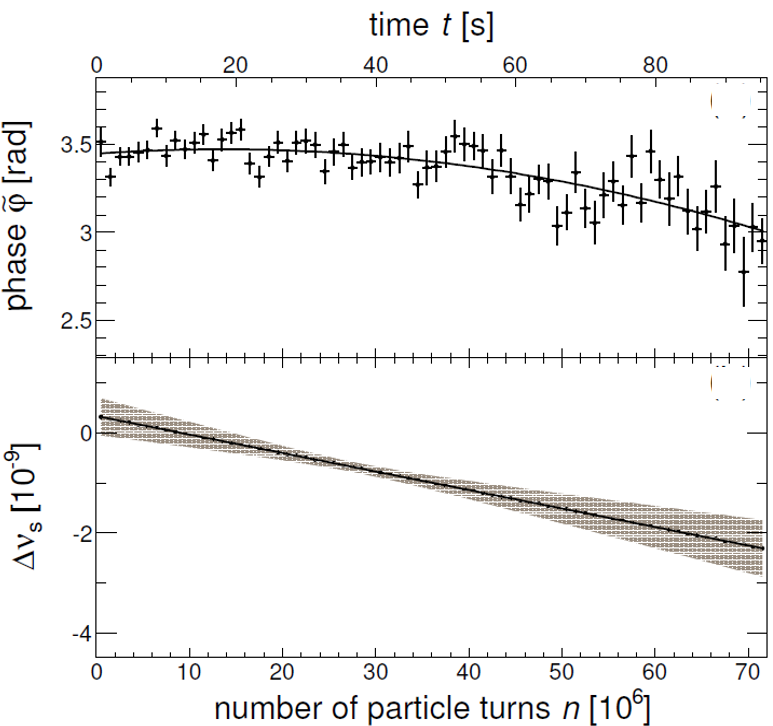
\includegraphics[width=0.9\textwidth]{spin-tune-determination.png}
\end{figure}
\end{columns}

\vspace{-0.2cm}
\begin{alertblock}{Experimental technique allows for:}
\begin{itemize}
 \item Spin tune $\nu_s$ determined to $\approx \num{e-8}$ in $\SI{2}{s}$ time interval.
 \item In a $\SI{100}{s}$ cycle at $t\approx \SI{38}{s}$, interpolated spin tune amounts to
            $|\nu_\text{s}| = (16097540628.3 \pm 9.7)\times 10^{-11}$, \textit{i.e.}, $\Delta \nu_s/\nu_s \approx \num{e-10}$.
 \item \textbf{$\Rightarrow$ new precision tool to study systematic effects in a storage ring.} 
\end{itemize}
\end{alertblock}

\end{frame}

\begin{frame}
\frametitle{Precision determination of the spin tune III}

\begin{columns}

 \column{0.7\textwidth}
 \begin{figure}
    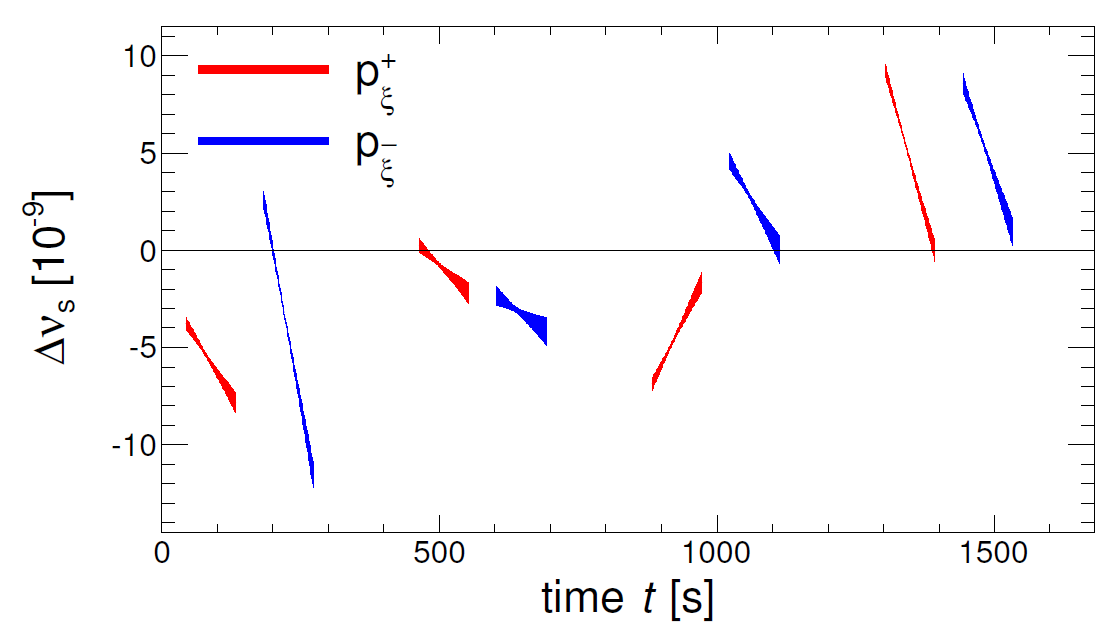
\includegraphics[width=1\textwidth]{spin-tune-walk.png}
 \end{figure}

\column{0.31\textwidth} 
\begin{small}
\begin{block}{}
   Walk of spin tune $\nu_s$ \textcolor{PineGreen}{\cite{PhysRevLett.115.094801}}.
\end{block}
\end{small}
\end{columns}


\begin{alertblock}{Applications of new technique:}
\begin{itemize}
 \item Study long term stability of an accelerator.
 \item Feedback system to stabilize phase of spin precession relative to phase of RF devices ($\rightarrow$  \textit{\textbf{phase-lock}}).
 \item Studies of machine imperfections.
\end{itemize}
\end{alertblock}

\end{frame}

\subsection{Phase locking}
\begin{frame}
\frametitle{Phase locking spin precession in machine to device RF}
 
\vspace{-0.2cm} 
\begin{block}{At COSY, one cannot freeze the spin precession}
 \begin{itemize}
  \item[$\Rightarrow$] To achieve precision for EDM, phase-locking is next best thing to do.
\end{itemize}
\end{block}
 
\vspace{-0.3cm}
\begin{columns}[t]
\column{0.44\textwidth} 
 
\begin{small} 
\vspace{-0.2cm}
\begin{exampleblock}{Feedback system maintains}
	\vspace{-0.2cm}
\begin{enumerate}
 \item resonance frequency, and
 \item phase between spin precession and  device RF (solenoid or WF)
\end{enumerate}
\end{exampleblock}
\end{small}

\vspace{-0.1cm}
\begin{figure}
     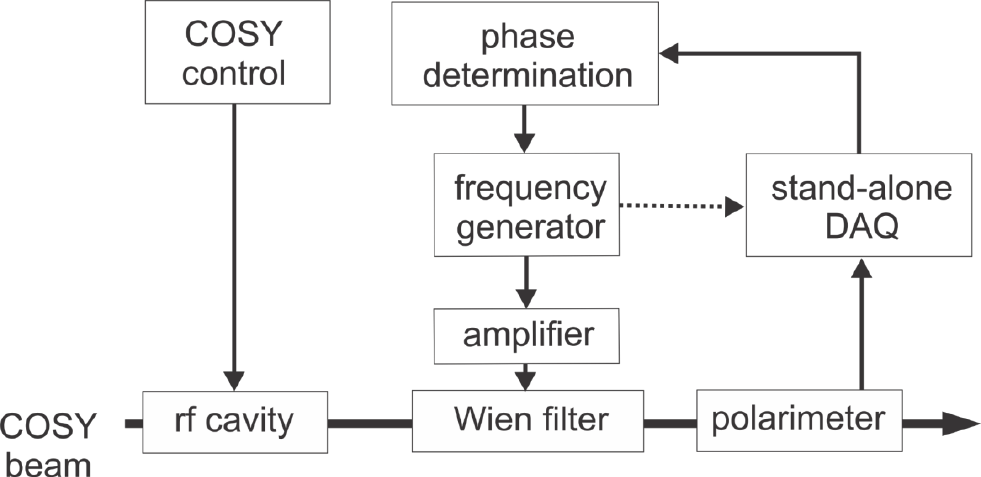
\includegraphics[width = 1\textwidth]{phase-lock-2.png}
\end{figure}

\column{0.5\textwidth} 
\vspace{-0.3cm}
\begin{figure}
     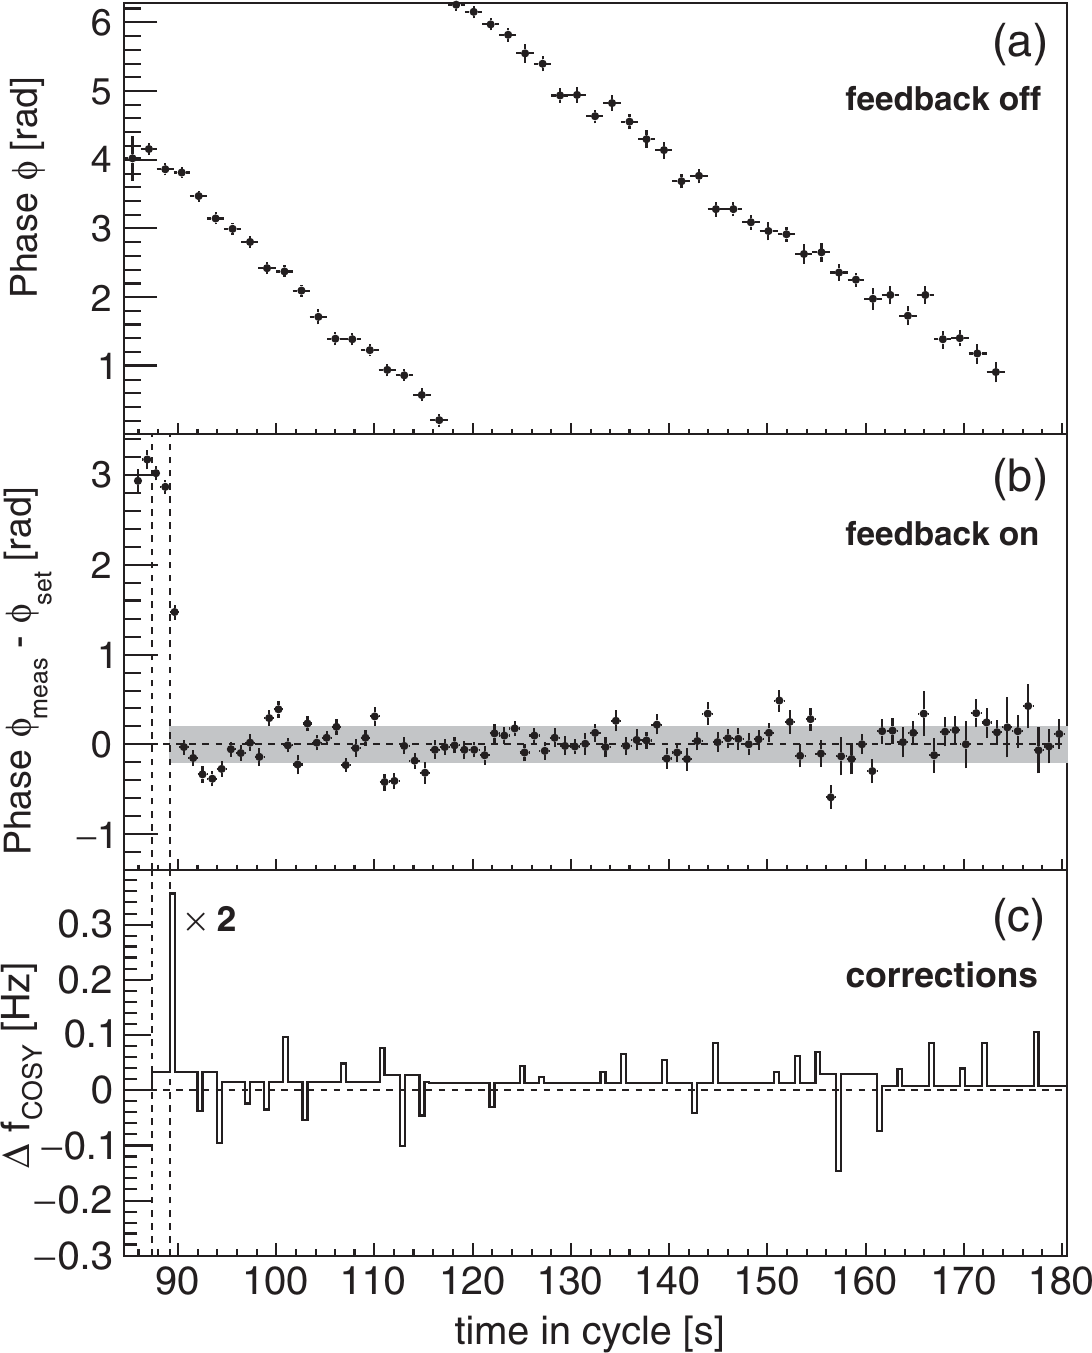
\includegraphics[width = 0.75\textwidth]{phase-locking-fig-1-from-PRL.png}
   \end{figure}
\end{columns}

\vspace{-0.2cm}
\begin{alertblock}{}
 \textbf{Major achievement} : Error of phase-lock $\sigma_\phi = \SI{0.21}{rad}$ \textcolor{PineGreen}{\small \cite{PhysRevLett.119.014801}}.
\end{alertblock}

\end{frame}

\subsection{RF Wien filter method}
\begin{frame}
\frametitle{Effect of EDM on stable spin axis of the ring \textcolor{PineGreen}{\cite{PhysRevAccelBeams.23.024601}}}
\framesubtitle{\textbf{Without accumulation (RF WF off)}}

\begin{columns}[c]
	
	\column{0.48\textwidth}
	\centering\includegraphics[width=0.9\textwidth]{stable-spin-axis.eps} 
	
	\column{0.5\textwidth}
	\vspace{-0.5cm}
	\begin{block}{\normalsize Beam particles move along $z$ direction}
		\begin{itemize}
			\item Presence of an EDM $\Rightarrow \xi_\text{EDM} > 0$.
			\item[$\Rightarrow$] Spins precess around the $\vec c$ axis.
			\item[$\Rightarrow$] Oscillating vertical polarization component $p_y(t)$ is generated.
		\end{itemize}
	\end{block}
	
\end{columns}

\vspace{0.5cm}
\begin{columns}[c]
	\column{0.48\textwidth}
	\centering\includegraphics[width=0.9\textwidth]{plot-WF-off-pz.eps} 
	
	\column{0.5\textwidth}
	\vspace{-0.5cm}
	\begin{block}{\normalsize Evolution for 10 turns [$\vec p_0 = (0,0,1)$]}
		\begin{itemize}
			\item $p_x(t)$, $p_z(t)$ and $p_y(t)$.
			\item Bunch revolution indicated as well. 
			\item $p_y$ oscillation amplitude corresponds to tilt angle $\xi_\text{EDM}$.
		\end{itemize}
	\end{block}
	
\end{columns}

\end{frame}
\begin{frame}
\frametitle{Model calculation of polarization buildup due to EDM \textcolor{PineGreen}{\cite{PhysRevAccelBeams.23.024601}}  }
\framesubtitle{\textbf{With RF Wien filter}}

\vspace{-0.3cm}
\begin{small}
\begin{block}{Ideal COSY ring with deuterons at $p_d = \SI{970}{MeV \per c}$:}
	\begin{itemize}
		\item $G = -0.143$,  $\gamma=1.126$, $\boxed{f_s = f_{\text{rev}} (\gamma G + K_{(=0)})} \approx \SI{120.765}{kHz}$ 
		\item Enhanced RF field integral $f_\text{ampl} \times \int E_{\text{WF}} \cdot \dd \ell \approx \SI{2200}{kV}$ (w/o ferrites) \textcolor{PineGreen}{\small \cite{Slim2016116}}.
	\end{itemize}
\end{block}
\vspace{-0.3cm}

\begin{figure}
	\includegraphics[height=0.36\textheight]{initial-slopes-from-different-EDMs.eps}
	\hspace{0.1cm}
	\includegraphics[height=0.36\textheight]{EDM-Resonance-Width-31012022afortalk2.eps}
\end{figure}

\vspace{-0.4cm}

\begin{alertblock}{Features of EDM induced vertical polarization buildup}
\begin{itemize}
	\item EDM accumulates in vertical polarization $p_y(t) \propto d$\,\textcolor{PineGreen}{\cite{PhysRevAccelBeams.20.072801,Rathmann:2013rqa,PhysRevLett.96.214802}}.
	\item $\rightarrow$ Full  oscillation of $p_y(t)$ with proper feedback via pilot bunch.
\end{itemize}	
\end{alertblock}

\end{small}
\end{frame}
\begin{frame}
\frametitle{Design of waveguide RF Wien filter} 
 
 \vspace{-0.2cm}
\begin{block}{ Joint Jülich -- RWTH Aachen development:}\small
\begin{itemize}
 \item Institute of High Frequency Technology, RWTH Aachen University:
%  \begin{itemize}
%   \item  Heberling, Hölscher, and PhD Student \textbf{Jamal Slim}, and ZEA-1 of Jülich. 
%   \end{itemize}
 \item \textbf{Waveguide provides $\vec E \times \vec B$ by design.}
  \item Minimal $\vec F_L$ by careful electromagnetic design of all components\,\textcolor{PineGreen}{\small \cite{Slim2016116, Slim201752, PhysRevAccelBeams.24.124601, PhysRevAccelBeams.26.014201}}.
\end{itemize}
\end{block}

\begin{figure}
    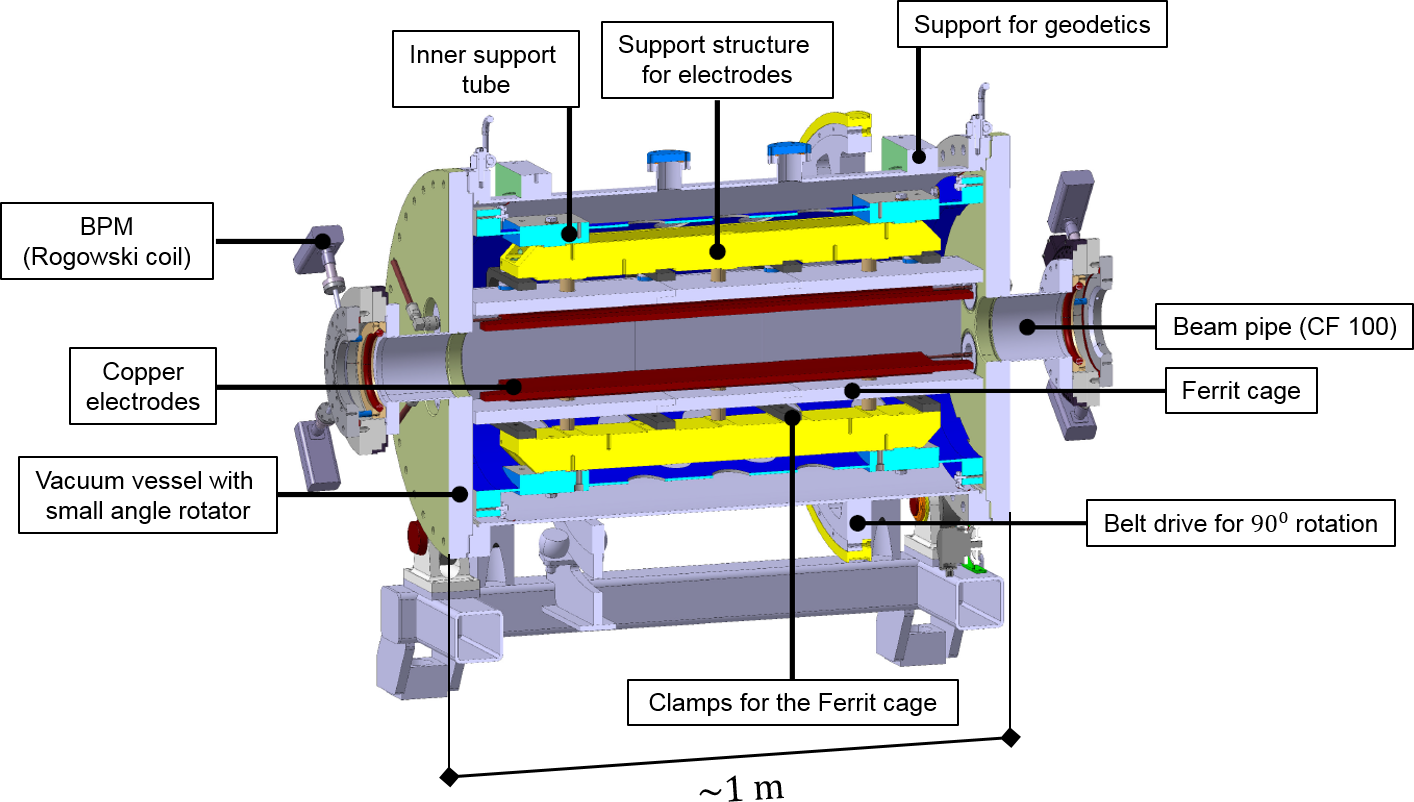
\includegraphics[height=0.38\textheight]{RF-Wien-features.png} \hspace{0.1cm}
    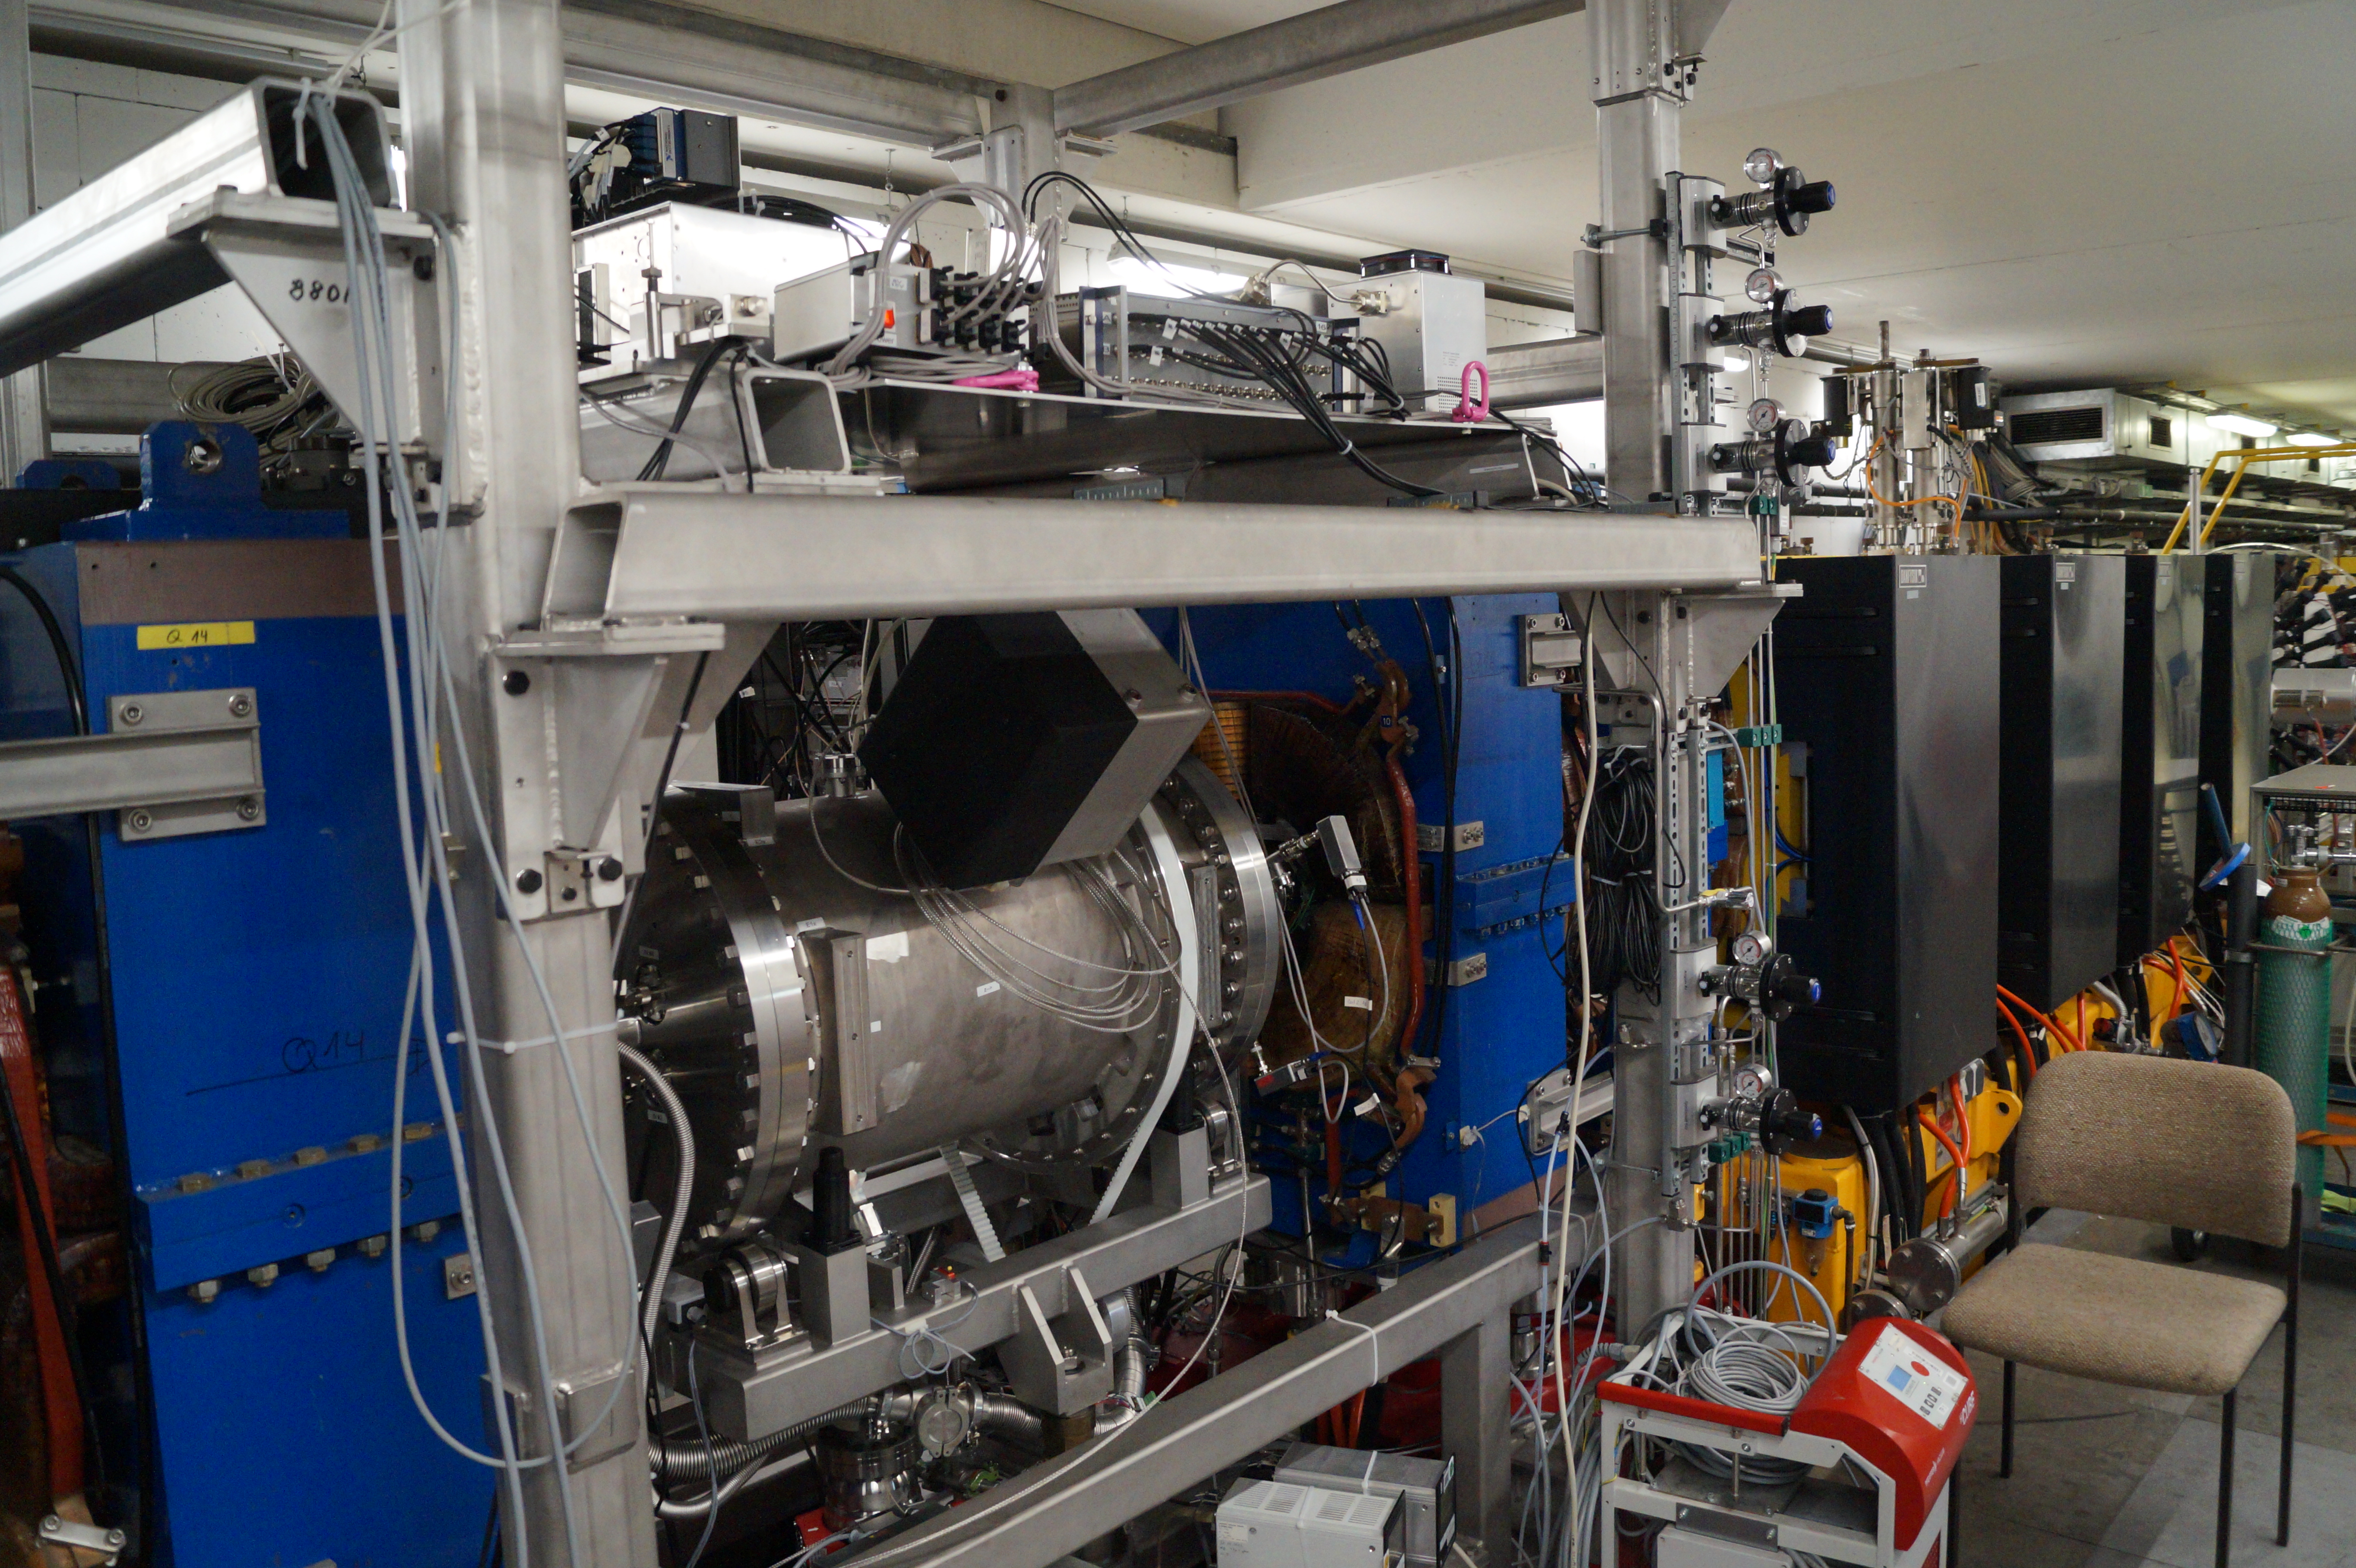
\includegraphics[height=0.38\textheight]{DSC09386.JPG}
\end{figure}

\end{frame}
\begin{frame}
\frametitle{View along the beam axis in the RF Wien filter}

\centering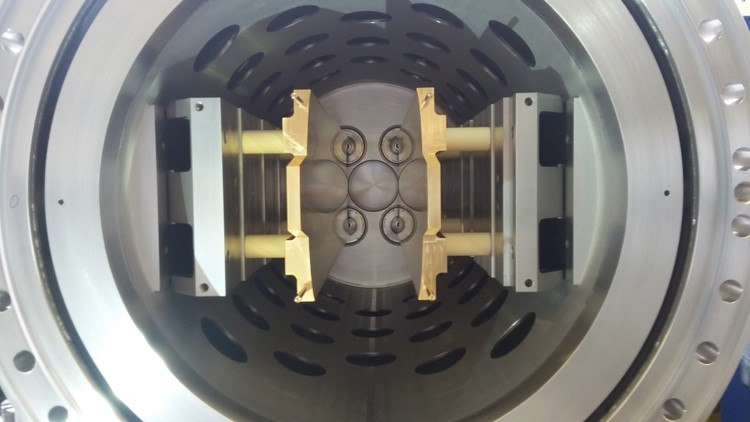
\includegraphics[height=0.75\textheight]{Bild4.jpg}

\end{frame}
%------------------------------------------------
\begin{frame}
 \frametitle{Bunch-selective spin manipulation $\rightarrow$ co-magnetometry I}
 \framesubtitle{\textbf{World-first (September 2020 JEDI, with $d$ at \SI{970}{MeV/c})} \textcolor{PineGreen}{\cite{Slim:2023lpd,Nikolaev:2023srx}}}

\vspace{-0.25cm}
\begin{columns}[c]
\column{0.4\textwidth} 
\begin{center}
 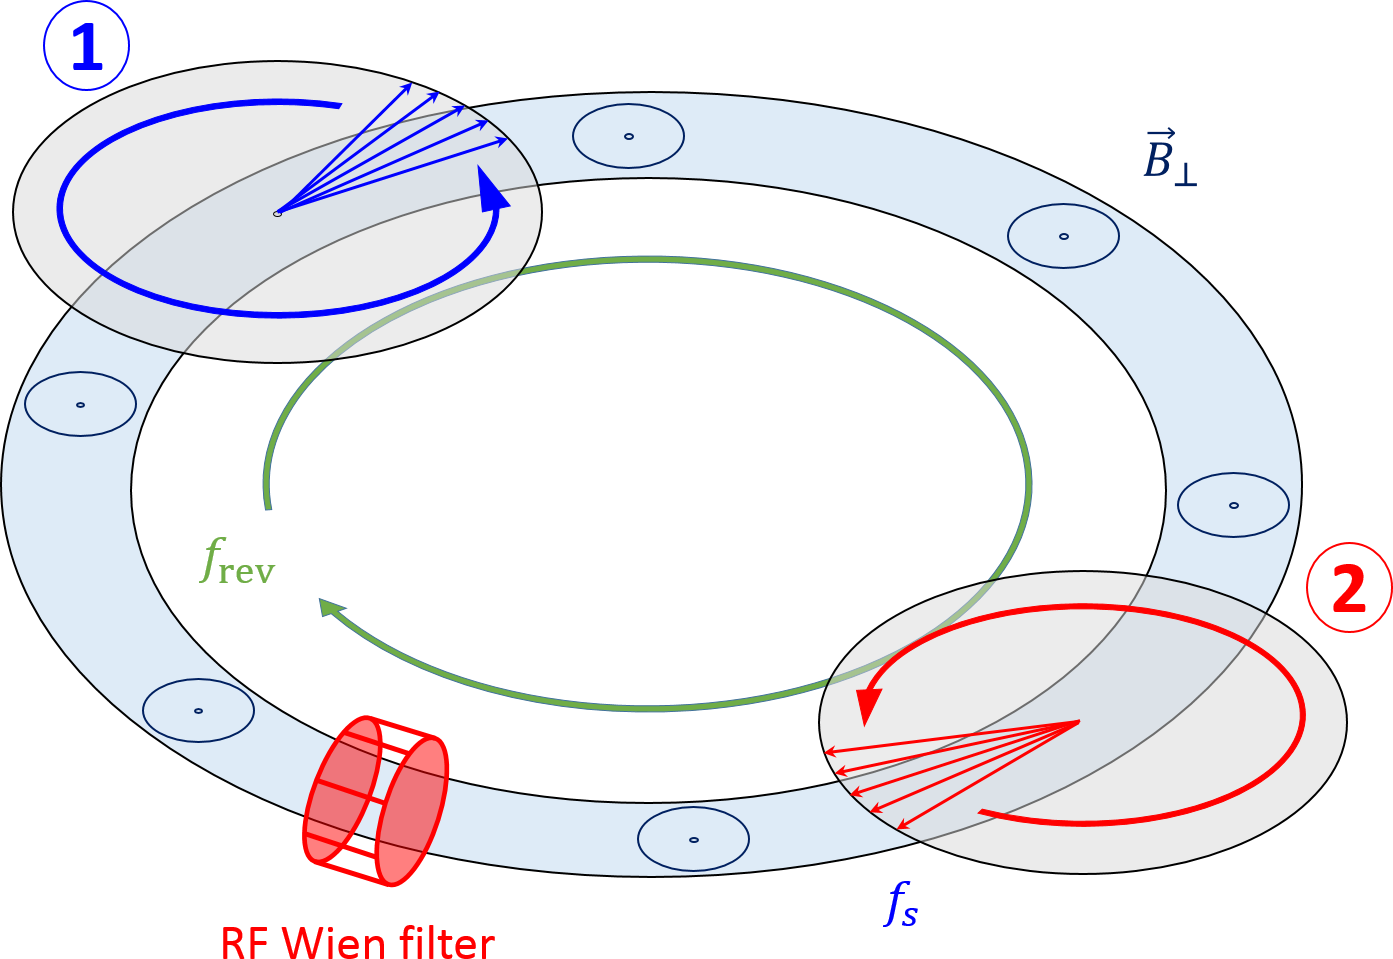
\includegraphics[height = 0.27\textheight]{spin-precession-3.png} 
\end{center}
 
\column{0.6\textwidth} 
\begin{small}
	\vspace{-0.25cm}
   \begin{itemize}
      \item signal\,\textcolor{blue}{\circled{\textbf{1}}} and pilot bunches\,\textcolor{red}{\circled{\textbf{2}}}:
      \begin{itemize}
          \item spin-coherent ensembles in ring plane orbit at $f_\text{rev} \approx \SI{750}{kHz}$
          \item precessing at $f_s \approx \SI{120}{kHz}$ 
      \end{itemize}
      \item waveguide RF WF\,\textcolor{PineGreen}{\cite{Slim2016116}} (\textit{radial} field $\vec B_r$), kept on resonance\footnotemark in\,\textcolor{blue}{\circled{\textbf{1}}} by spin tune measured in\,\textcolor{red}{\circled{\textbf{2}}}
   \end{itemize}
\end{small}
\end{columns}

\vspace{0.2cm}
\begin{small}
\textbf{\textit{Selective} gating of one of the two stored bunches at RF Wien filter: }
      \begin{itemize}
       \item[\textcolor{blue}{\circled{\textbf{1}}}] RF WF enhancement of  $p_y(t)$ of \textcolor{blue}{signal bunch}
       \item[\textcolor{red}{\circled{\textbf{2}}}] \textcolor{red}{pilot bunch}, unperturbed by RF WF, acts as co-magnetometer
      \end{itemize}
\end{small}

\footnotetext[1]{$f_{\mathrm{WF}}  =   K\cdot f_\text{rev} + f_s = (K + \nu_s)f_\text{rev}$, where $K \in \mathbb{Z}$ and  $\nu_s$ spin tune, $f_\text{WF}^{(K=-1)} \approx  \SI{871.431}{kHz}$} 

\vspace{-0.6cm}
\begin{columns}[T]
\column{0.48\textwidth} 
\begin{center}
   \includegraphics[height = 0.28\textheight]{bunches2DNorm_19082023.pdf} 
\end{center}


\column{0.48\textwidth} 
\begin{center}
    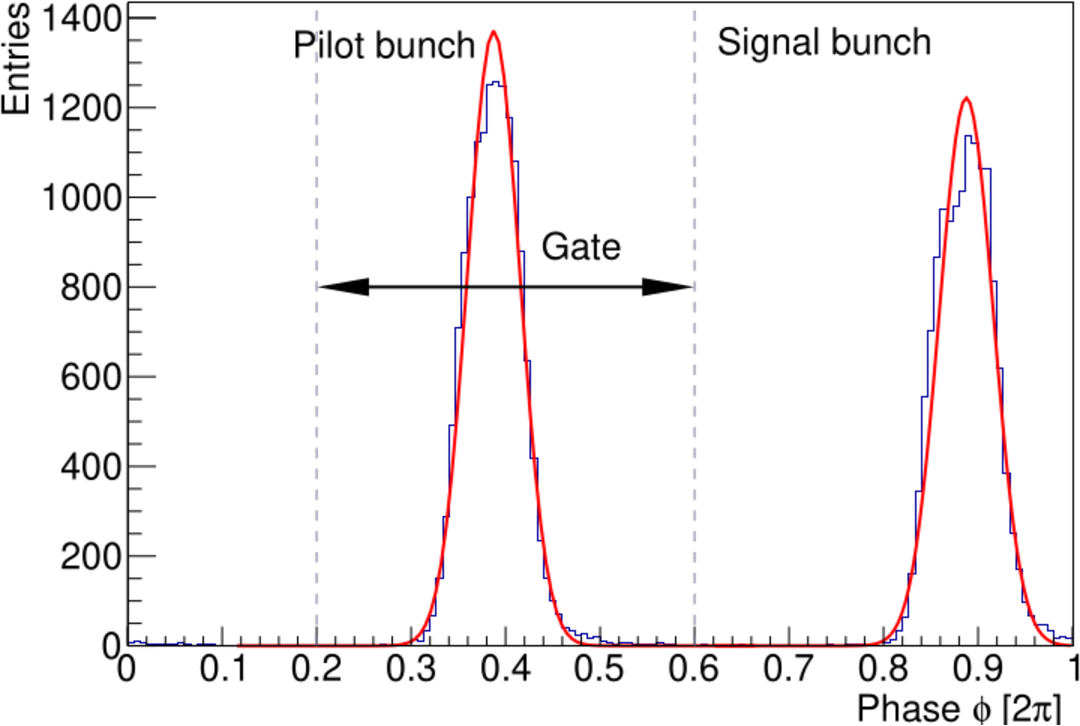
\includegraphics[height = 0.28\textheight]{bunches122_19082023.pdf} 
\end{center}

\end{columns}
 
\end{frame}

%------------------------------------------------
\begin{frame}
 \frametitle{Fast switches\footnote{developed together with Fa.\ barthel HF-Technik GmbH, Aachen} for RF power of Wien filter}
 
\vspace{-0.2cm} 
\begin{columns}
 \column{0.52\textwidth}
\begin{small}
\textbf{GaN HEMT-based solution (Gallium Nitride Transistors):}
 \begin{itemize}
    \item Short switch on/off times ($\approx$ few ns).
    \item High power capabilities ($\approx$ few kV).
    \item On board power damping.
  \end{itemize}
\end{small}
 
 \column{0.5\textwidth}
 \begin{center}
  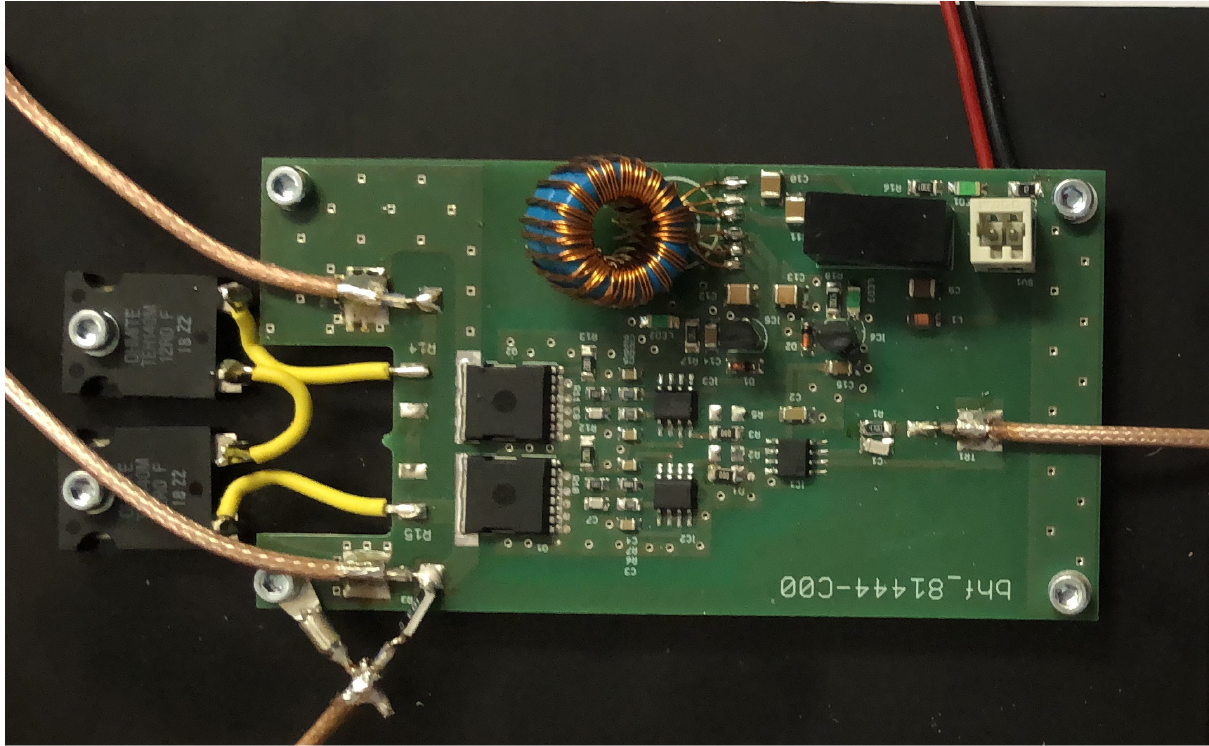
\includegraphics[width = 0.75\textwidth]{fast-switch}
 \end{center}
\end{columns}
 
\vspace{-0.4cm} 
\begin{columns}
 \column{0.46\textwidth}
  \begin{center}
  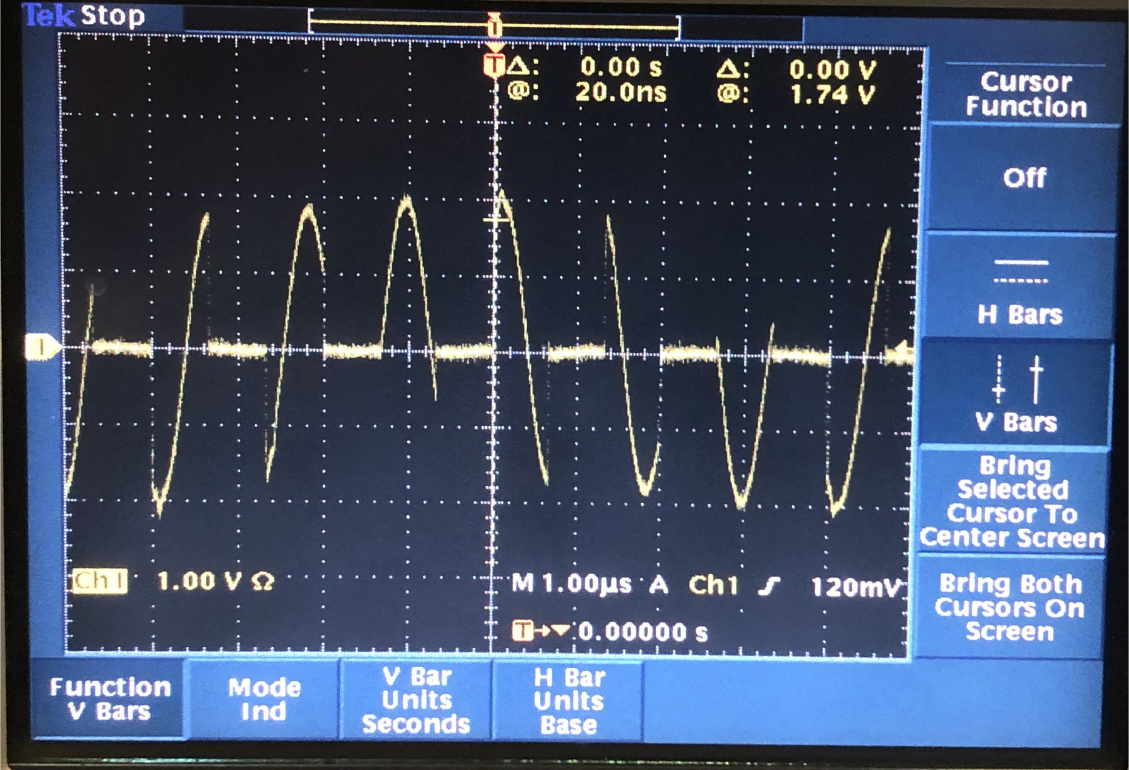
\includegraphics[width = 0.75\textwidth]{osci-fast-switch}
 \end{center}
 
 \column{0.54\textwidth}
\begin{small}
 \begin{itemize}
 \item symmetric switch on/off times ($\approx$ few ns).
 \item $-\SI{30}{\decibel}$ power damping.
  \end{itemize}
\end{small}
\end{columns}

\vspace{-0.2cm}  
\begin{alertblock}{Installed switches:}
\begin{itemize}
 \item capable to handle up to \SI{200}{W} each
 \item permits system to run near a total power of \SI{0.8}{kW} in pulsed mode
\end{itemize}
\end{alertblock}
  

\end{frame}
%------------------------------------------------

%------------------------------------------------
\begin{frame}
 \frametitle{Implementation of fast switches\footnote{developed together with Fa.\ barthel HF-Technik GmbH, Aachen} at RF Wien filter}	
 \framesubtitle{Modification of driving circuit\,\textcolor{PineGreen}{\cite{Slim:2020ufk}}}
 
\vspace{-0.3cm}  
\begin{center}
 	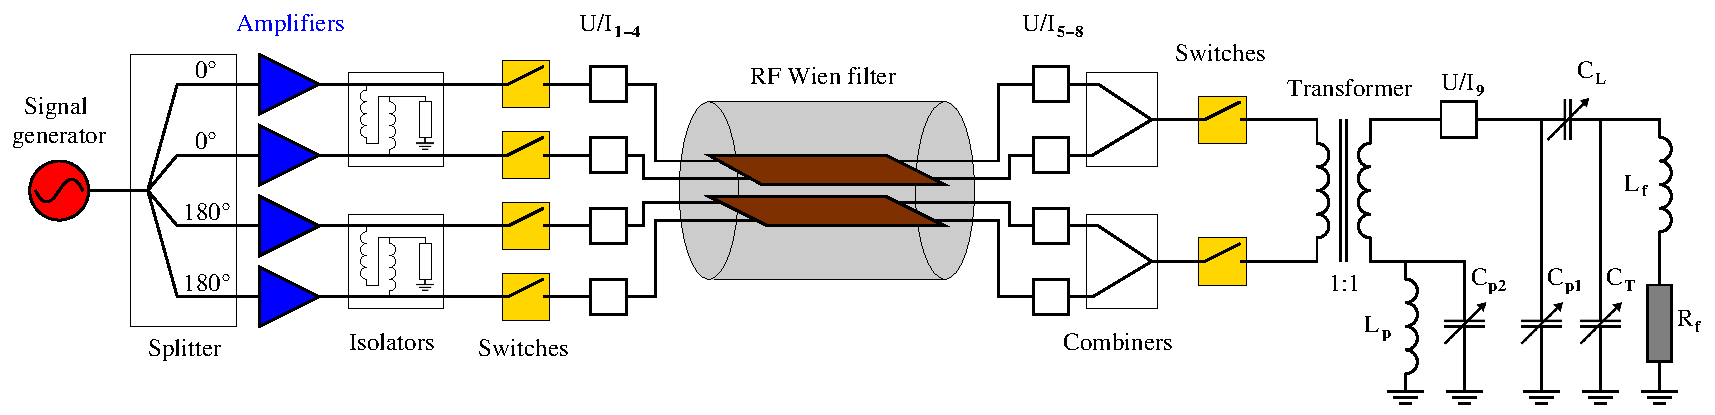
\includegraphics[width = 1\textwidth]{drivingcircuit-switches-1.pdf}
\end{center}
 
\vspace{-0.3cm} 
\begin{columns}
 \column{0.6\textwidth}
\begin{small}
\textbf{GaN HEM FET-based solution:}
 \begin{itemize}
    \item Short switch on/off times ($\approx$ few ns).
    \item High power capabilities ($\approx$ few kV).
    \item On board power damping ($-\SI{30}{\decibel}$ ).
    \item Symmetric switch on/off times ($\approx$ few ns).
  \end{itemize}
\end{small}
 
\column{0.35\textwidth}
\begin{center}
  \includegraphics<1>[height = 0.6\textwidth]{fast-switch}
  \includegraphics<2>[height = 0.6\textwidth]{gating_15052023.pdf}
  \end{center}
\end{columns}

\begin{alertblock}{Switches}
\begin{itemize}
 \item capable to handle up to \SI{200}{W} each
 \item permits system to run near a total power of \SI{0.8}{kW} in pulsed mode
\end{itemize}
\end{alertblock}
  
\end{frame}
%------------------------------------------------

\begin{frame}
 \frametitle{Bunch-selective spin manipulation $\rightarrow$ co-magnetometry II}
\framesubtitle{\textbf{World-first (September 2020 JEDI, with $d$ at \SI{970}{MeV/c}) }}

\vspace{-0.2cm}
See recent JEDI preprints for more details: 
\begin{footnotesize}
\begin{itemize}
	\item \textit{Pilot bunch and co-magnetometry of polarized particles stored in a ring}\,\textcolor{PineGreen}{\cite{Slim:2023lpd}}
	\item \textit{Spin decoherence and off-resonance behavior of radiofrequency-driven spin rotations in storage rings}\,\textcolor{PineGreen}{\cite{Nikolaev:2023srx}}
\end{itemize}
\end{footnotesize}

\vspace{-0.3cm}
\begin{columns}[T]
\column{0.42\textwidth}
\only<1>{
\begin{block}{\small Exponential model\,\textcolor{PineGreen}{\small \cite{Slim:2023lpd}}:}
\begin{equation}
\begin{split}
A(t) = \, & a (t-t_0) + b \, + \\
       & c  \exp\left(- \Gamma (t-t_0)\right) \\
       & \cos\left[2\pi f_\text{SF} (t-t_0)\right]
\nonumber
\end{split}
\end{equation}
\end{block}}

\only<2>{
\begin{block}{\small Synchrotron-oscillations model\,\textcolor{PineGreen}{\small \cite{Nikolaev:2023srx}}:}
\begin{small}
\begin{equation}
\begin{split}
A_\text{sy}(t) = & a (t-t_0) + b
+ \\ & 
\frac{c}{\sqrt{1+ \left[ 2\pi Q_\text{sy} f_\text{SF} (t-t_0) \right] ^2}} 
\times \\
&\cos \big[ 2\pi f_\text{SF} (t-t_0)  - \\
& \arctan(2\pi Q_\text{sy} f_\text{SF} (t-t_0) ) \big]
\label{SO-fit}
\nonumber
\end{split}
\end{equation}
\end{small}
\end{block}}

\column{0.51\textwidth}
\begin{center}
	\vspace{-0.3cm}
	\includegraphics<1>[height = 0.43 \textheight]{fit_exp_19082023.pdf} 
	\includegraphics<2>[height = 0.43 \textheight]{2sg1_19082023.pdf} 
\end{center}
\end{columns}

\vspace{-0.1cm}  
\begin{alertblock}{Works close to perfection}
	\begin{itemize}
		\item allows spin manipulations on \textit{individual} stored bunches \textbf{on flattop}
		\item application of principle on the horizon for EIC and NICA
	\end{itemize}
\end{alertblock}
 \end{frame}

\section{Recent results}
\subsection{EDM measurement}

\begin{frame}
\frametitle{Strength of EDM resonance}

\vspace{-0.2cm}
\begin{columns}
	\column{0.5\textwidth}
	\begin{block}{\normalsize \textbf{EDM induced  polarization oscillation,}}
		\begin{itemize}
			\item  can generally be described by 
			\begin{equation}
			p_y(t)  = a \, \sin ( \Omega^{p_y} \, t + \phi_\text{RF}) \,, \nonumber
			\label{eq:initial-slope-from-full-oscillation}
			\end{equation}
			$y$ perpendicular to ring plane.
			
			\item \textbf{EDM resonance strength} defined as ratio of angular frequency $\Omega^{p_y}$ to  orbital angular frequency $\Omega^\text{rev}$\,\textcolor{PineGreen}{\small \cite{PhysRevAccelBeams.23.024601}},
			\begin{equation}
			\varepsilon^\text{EDM} = \frac{\Omega^{p_y}}{\Omega^\text{rev}}\,, \nonumber
			\label{eq:resonance-strength}
			\end{equation}
		\end{itemize}
	\end{block}
	
	\column{0.5\textwidth}
	\begin{figure}
		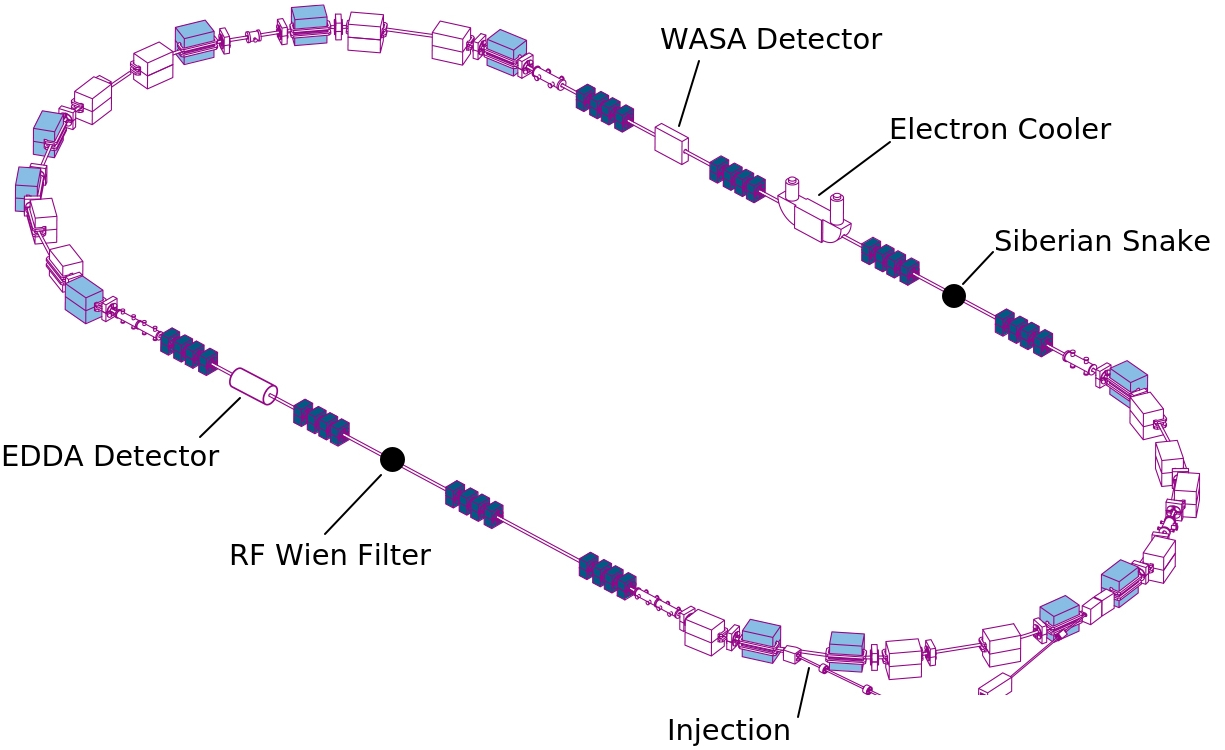
\includegraphics[width=0.95\textwidth]{COSY-landscape.jpg}
	\end{figure}
\end{columns}

\begin{block}{How is the EDM effect actually measured?}
	Two \textit{simultaneously} applied spin rotations, one in each opposite straight section:
	\begin{enumerate}
		\item \textbf{RF Wien filter} magnetic axis ($\vec e_z^\perp$) rotated by small angle $\rightarrow$ generates radial magnetic RF field about which spins precess.
		\item Longitudinal magnetic field of \textbf{Siberian snake}  opposite to Wien filter $\rightarrow$ rotates spins about $\vec e_z$.
	\end{enumerate}
\end{block}

\end{frame}
\begin{frame}
\frametitle{Measurement of EDM resonance strength using pilot bunch}
\framesubtitle{RF Wien filter mapping}

Observation of $p_y(t)$ with two stored bunches: \textbf{Signal and pilot bunch (PB)}

\begin{itemize}
	\item Signal bunch
	\begin{center}
		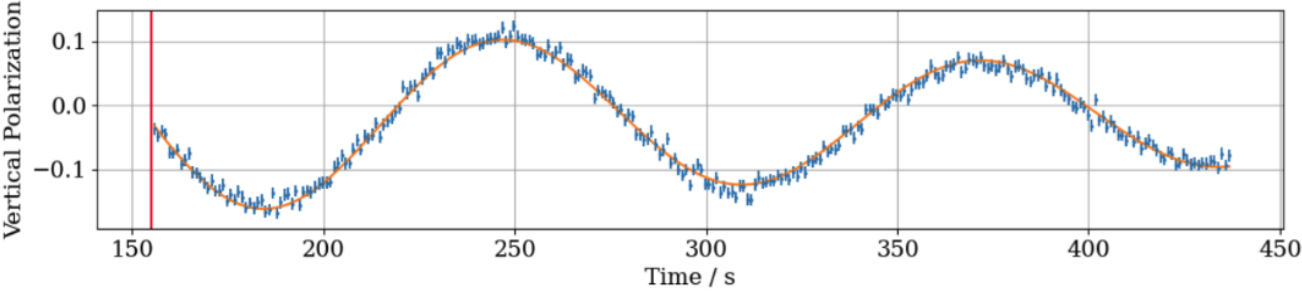
\includegraphics[width=0.75\textwidth]{precursor-2-signal-bunch.png}
	\end{center}
	\item Pilot bunch
	\begin{center}
		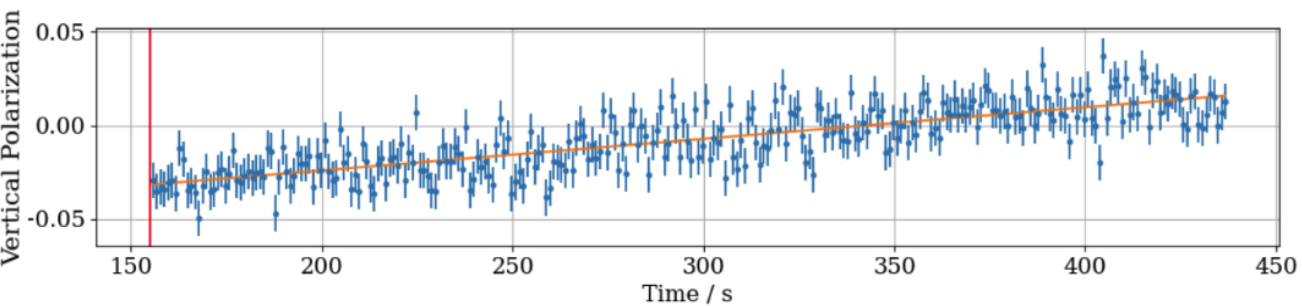
\includegraphics[width=0.75\textwidth]{precursor-2-pilot-bunch.png}
	\end{center}
\end{itemize}

\begin{small}
	\begin{itemize}
		\item Decoherence clearly visible in signal bunch.
		\item No oscillations in pilot bunch.
		\item Determine oscillation frequencies $\Omega^{p_y}$ $\rightarrow$ Wien filter map via $\varepsilon^\text{EDM} = \frac{\Omega^{p_y}}{\Omega^\text{rev}}$
	\end{itemize}
\end{small}

\end{frame}

\begin{frame}
\frametitle{Measurement of EDM resonance strength using pilot bunch}
\framesubtitle{Polarization evolution of signal bunch during measurement cycle}
	
\textbf{Combined fit ($p_y$, $p_{xz}$, phasewalk)} by Vera Shmakova (see her talk from Mo)	

\vspace{-0.2cm}	
\begin{columns}
\column{0.35\textwidth}
\begin{center}
	\hfill $p_y(t)$
\end{center}
\column{0.6\textwidth}
\begin{center}
	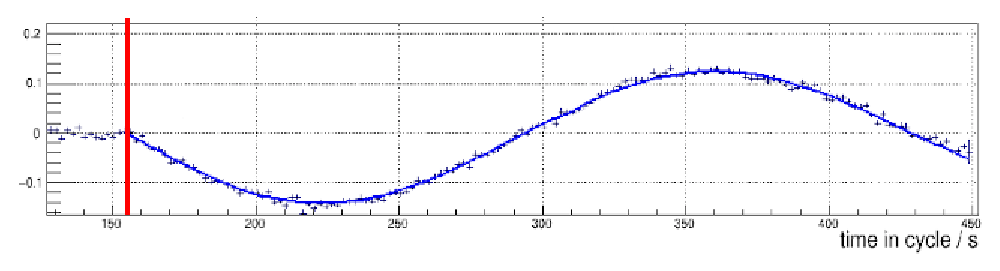
\includegraphics[width=0.8\textwidth]{vera_combined_fit_slide-extract-py.eps}
\end{center}
\end{columns}
	
\vspace{-0.2cm}
\begin{columns}
\column{0.35\textwidth}
	\hfill $p_{xz}(t)$
\column{0.6\textwidth}
\vspace{-0.3cm}
\begin{center}
	\includegraphics[width=0.8\textwidth]{vera_combined_fit_slide-extract-pxz.eps}
\end{center}
\end{columns}	

\begin{columns}
\column{0.35\textwidth}
\hfill in-plane phase walk of $p_{xz}(t)$
\column{0.6\textwidth}
\vspace{-0.3cm}
\begin{center}
	\includegraphics[width=0.8\textwidth]{vera_combined_fit_slide-extract-phase.eps}
\end{center}
\end{columns}	
	
\begin{alertblock}{\small Extensive analysis of 3D polarization evolution in recent preprint, N.N.\,Nikolaev et al.\,\textcolor{PineGreen}{\cite{Nikolaev:2023srx}} }
\begin{itemize}
	\item vertical and in-plane polarization evolution, phase walk, 
	off-resonance behavior, finite-spin coherence and synchrotron-oscillation effects
\end{itemize}
\end{alertblock}	
	
\end{frame}
\begin{frame}
\frametitle{Results from dEDM precursor experiment}
\framesubtitle{Precursor I: 3 maps with initial-slope method (IS). Precursor II: 2 maps IS + 5 maps with PB}

\vspace{-0.1cm}
\textbf{EDM resonance strength map for $\varepsilon^\text{EDM}$, includes tilts of invariant spin axis due to EDM and magnetic ring imperfections.}

\begin{columns}[T]
\column{0.45\textwidth}
\vspace{-0.2cm}
\begin{center}
	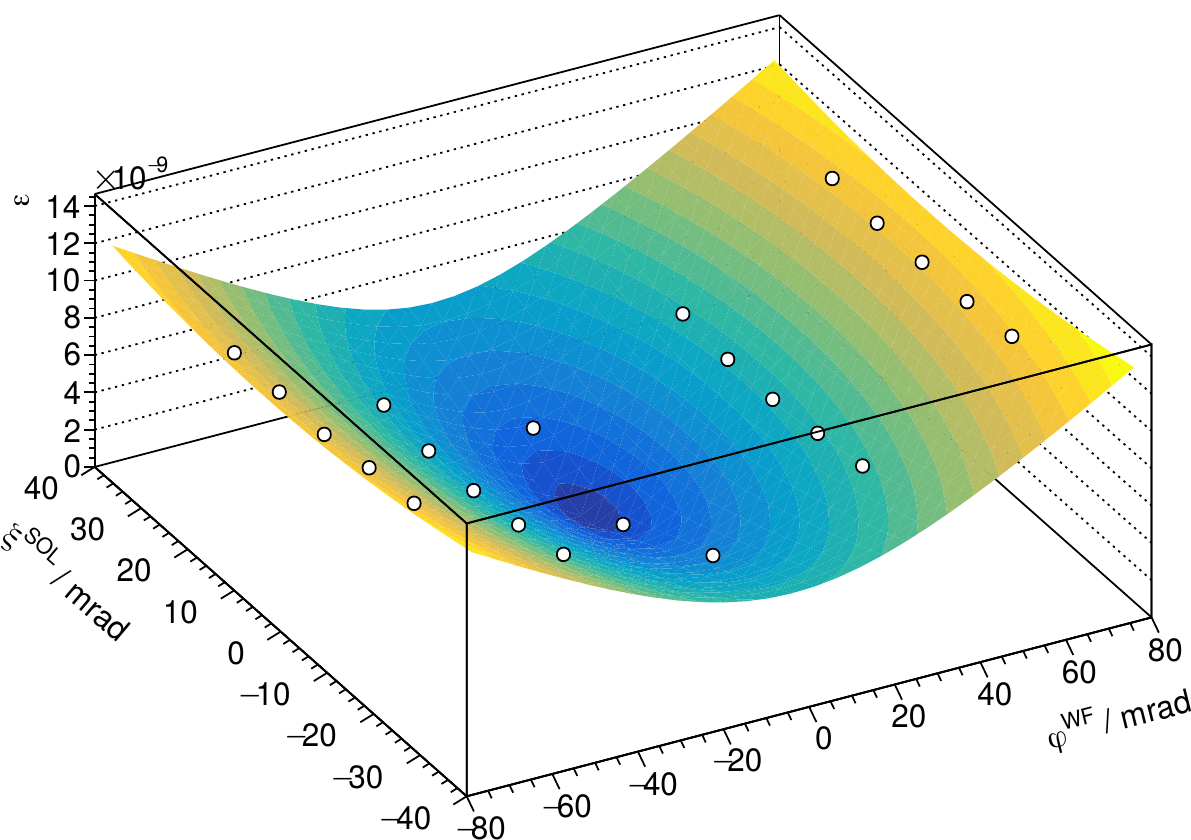
\includegraphics[width=0.7\textwidth]{map4.png}
	\vspace*{-20ex}\hspace*{-1.5cm}  % Tune this to the image height.
	\begin{center}
		\textcolor{red}{preliminary}
	\end{center}
	\vspace*{20ex}\hspace*{1.5cm}
\end{center}
\vspace{-0.2cm}
\column{0.55\textwidth}
Determination of minimum via fit with theoretical surface function yields: 
\begin{itemize}
	\item $\color{ForestGreen}{\boxed{\phi_0^\text{WF} / \text{mrad} = 2.51 \pm 0.04}}$ 
	\item  $\color{Maroon}{\boxed{\xi_0^\text{Sol} / \text{mrad} = -3.93  \pm 0.06}}$
\end{itemize}
\small Analysis by Vera Shmakova and Achim Andres
\end{columns}	

\vspace{-1.4cm}
\begin{block}{\small \textbf{Extraction of deuteron EDM:}}
\vspace{-0.1cm}	\begin{enumerate}
	\item Minimum determines spin rotation axis (3-vector) at RF WF, \textit{including EDM}.
	\item Spin tracking in COSY lattice $\rightarrow$ orientation of stable spin axis \textit{w/o} EDM.
	\item EDM is obtained from the difference of 1.\ and 2.
\end{enumerate}
\end{block}

\vspace{-0.3cm}
\begin{alertblock}{\small \textbf{EDM analysis now focuses more on systematics}}
\begin{itemize}
	\item Data analysis close to final \& EDM results in preparation.
	\item Goal: Describe observed tilts of stable spin axis by spin tracking. 
\end{itemize}
\end{alertblock}

\end{frame}


\subsection{Axion measurement}
\begin{frame}
\frametitle{Measurement of axion-like particle in storage ring}
\framesubtitle{\textbf{First-ever search for axion-like particles using this method}}


\begin{block}{Basic idea}
	\begin{itemize}
		\item Axion field \textcolor{Maroon}{$a(t) = a_0\cos\left( \omega_a (t-t_0) + \phi_a(t_0) \right)$} \newline
		induces an oscillating EDM\,\textcolor{PineGreen}{\small \cite{PhysRevD.84.055013}} \textcolor{Maroon}{$d(t) = d_\text{DC} + d_\text{AC}\cos\left( \omega_a (t-t_0) + \phi_a(t_0) \right)$} \newline
		with frequency related to axion mass via \textcolor{Maroon}{$\hbar \omega_a = m_a c^2$}, $f_a$ is decay constant.
		\item This affects the spin rotations in the ring,
		$$ \frac{\dd S}{\dd t} = \left(\vec \Omega_\text{MDM} - \vec \Omega_\text{rev} + \vec \Omega_\text{EDM} + \vec \Omega_\text{wind} \right)\times \vec S\,, $$
		because two axion-related terms enter: (EDM:\,\textcolor{PineGreen}{\small \cite{PhysRevD.84.055013}}, wind:\,\textcolor{PineGreen}{\small \cite{PhysRevD.88.035023}})
		{\color{Maroon}
		\begin{equation}
		\begin{split} 
		\vec \Omega_\text{EDM} & =  -\frac{1}{S \hbar} d(t) c \vec \beta \times \vec B\,, \quad \text{and} \\ 
		\vec \Omega_\text{wind} & = -\frac{1}{S \hbar} \frac{C_N}{2 f_a} \left( \hbar \partial_0 a(t) \right)  \vec \beta \quad \biggl\{ {{\text{coupling constant}\, C_N} \atop {\text{time derivative}\, \partial_0}}
		\end{split}
		\end{equation}}
	 \end{itemize}
\end{block}


\begin{alertblock}{}  
\textbf{$\Rightarrow$ Resonant build-up of vertical polarization, when \textcolor{Maroon}{$\omega_a = \omega_s$}}	
%Buildup proportional to  and axion phase is favorable (used 4 bunches with different spin orientations).
\end{alertblock}

\end{frame}

\begin{frame}
\frametitle{Details about axion/ALP experiment 
(\textcolor{PineGreen}{\cite[PRX]{PhysRevX.13.031004}} I}

\vspace{-0.3cm}
\begin{block}{Momentum  ramps ($f_\text{rev}$) in COSY searching for polarization changes}

\begin{columns}
	\column{0.45\textwidth}
	\vspace{-0.3cm}
	\begin{figure}
		\centering
		\vspace{-0.5cm}
		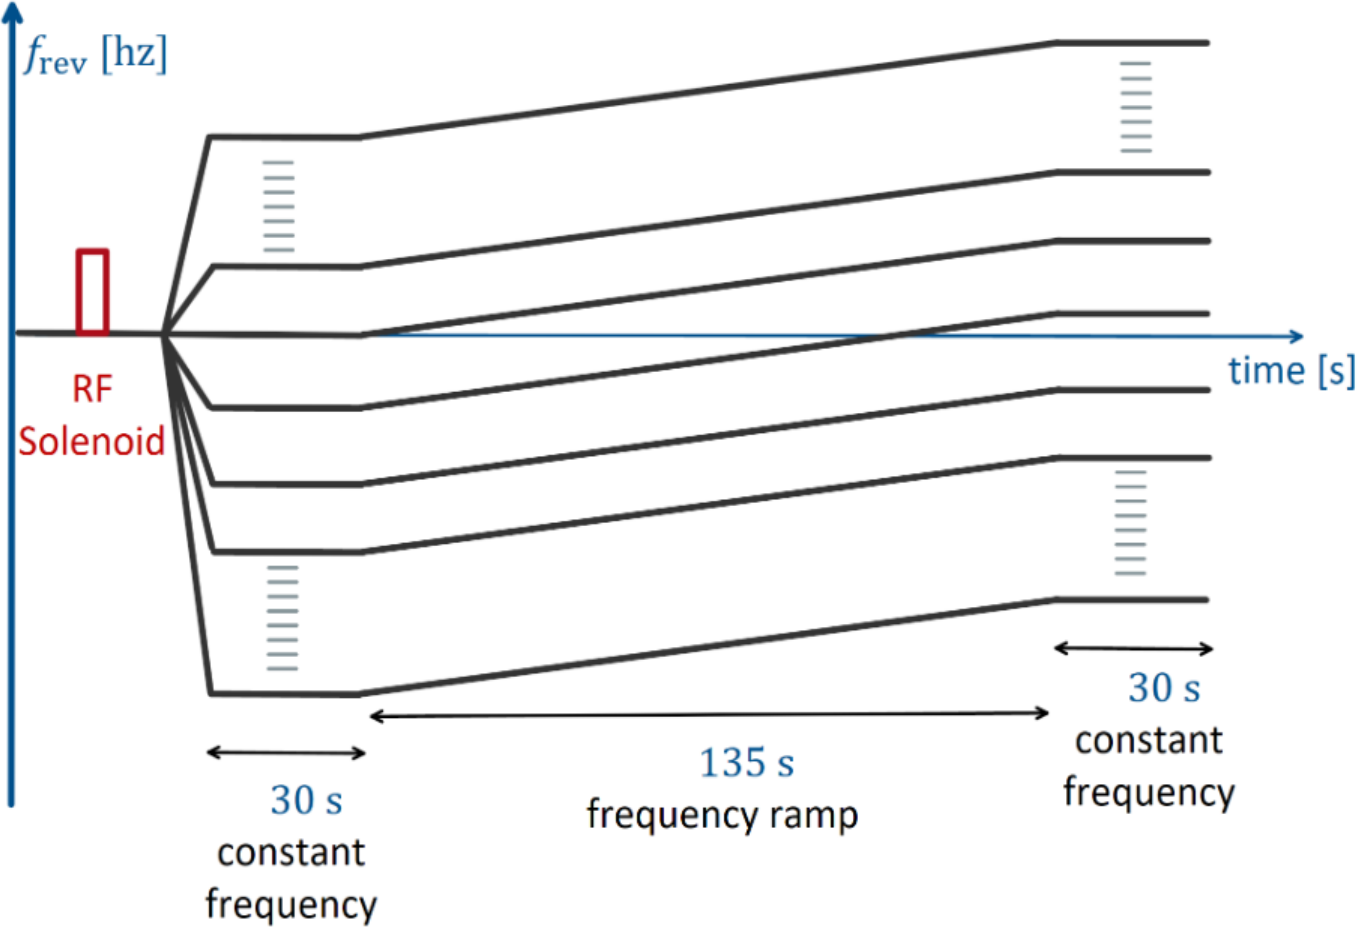
\includegraphics[height=0.4\textheight]{frequency-ramps-COSY.png} 
		\caption{Organization of frequency ramps}
	\end{figure}
	\vspace{-0.6cm}
		
	\column{0.45\textwidth}
	\vspace{-0.3cm}
	\begin{figure}	
		\centering
		\vspace{-0.1cm}
		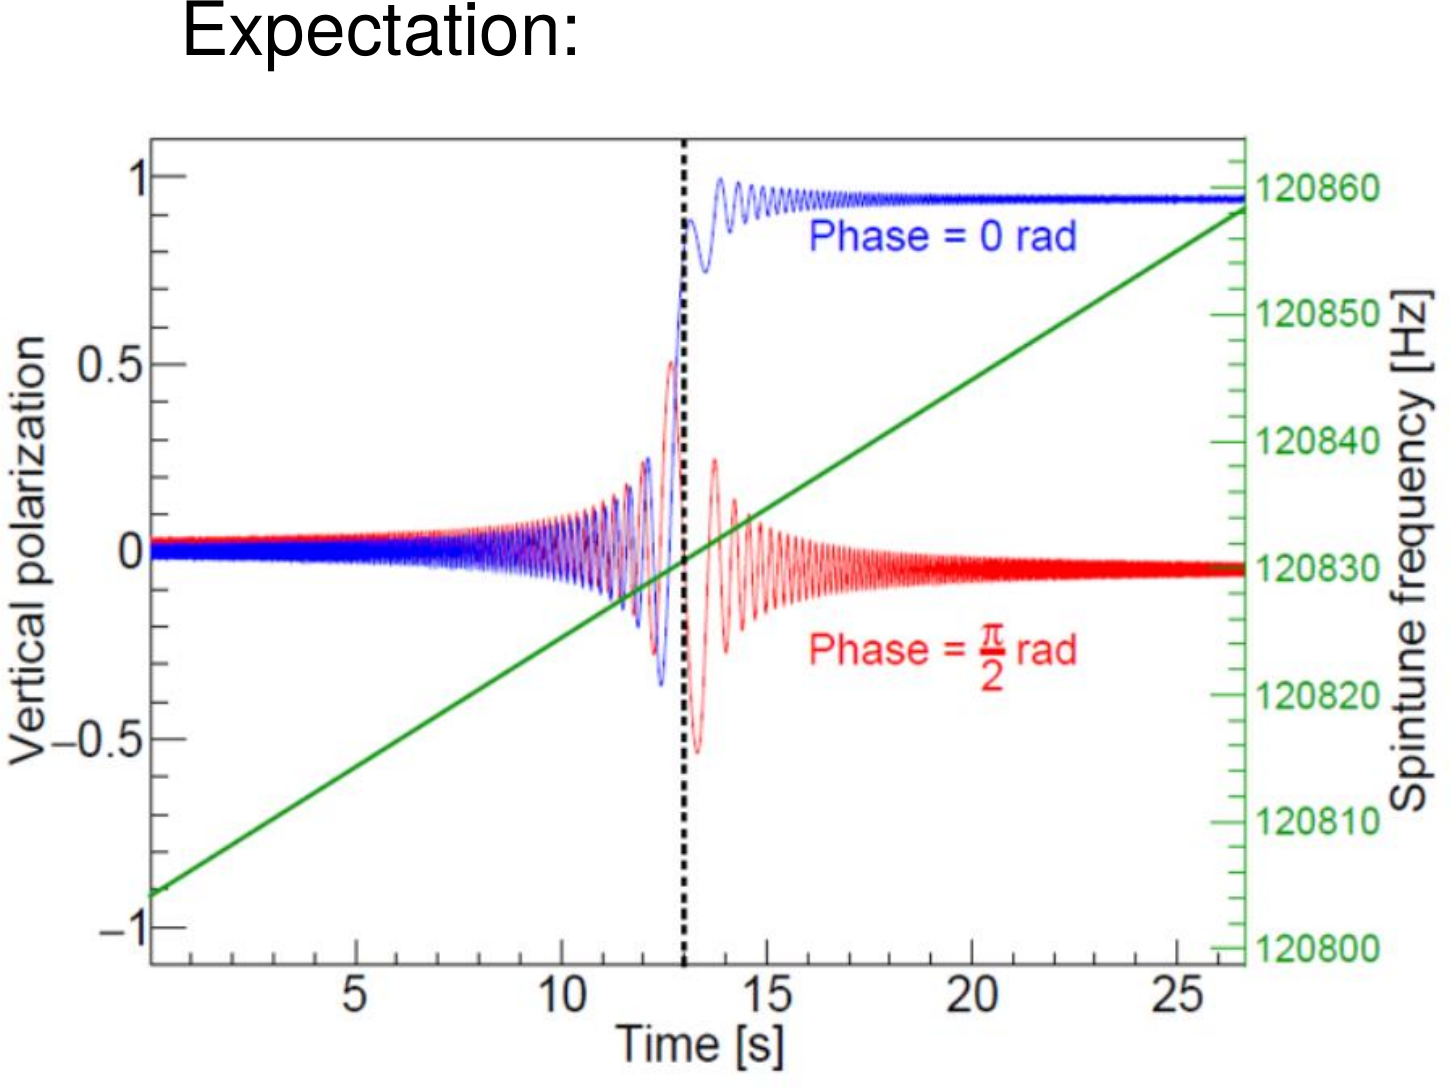
\includegraphics[height=0.4\textheight]{polarization-expectation-in-ramp.png}
		\caption{Jump of vertical polarization jump when resonance is crossed, for $\omega_a = \omega_s$.}
	\end{figure}
	\vspace{-0.6cm}
\end{columns}
\end{block}

\end{frame}

\begin{frame}
\frametitle{Details about axion/ALP experiment 
(\textcolor{PineGreen}{\cite[PRX]{PhysRevX.13.031004}} II}

\begin{block}{Cover different oscillating EDM phases using multiple bunches}
	\begin{columns}
		
		\column{0.45\textwidth}
		\vspace{-0.3cm}
		\begin{figure}
		\centering
		\vspace{-0.2cm}
		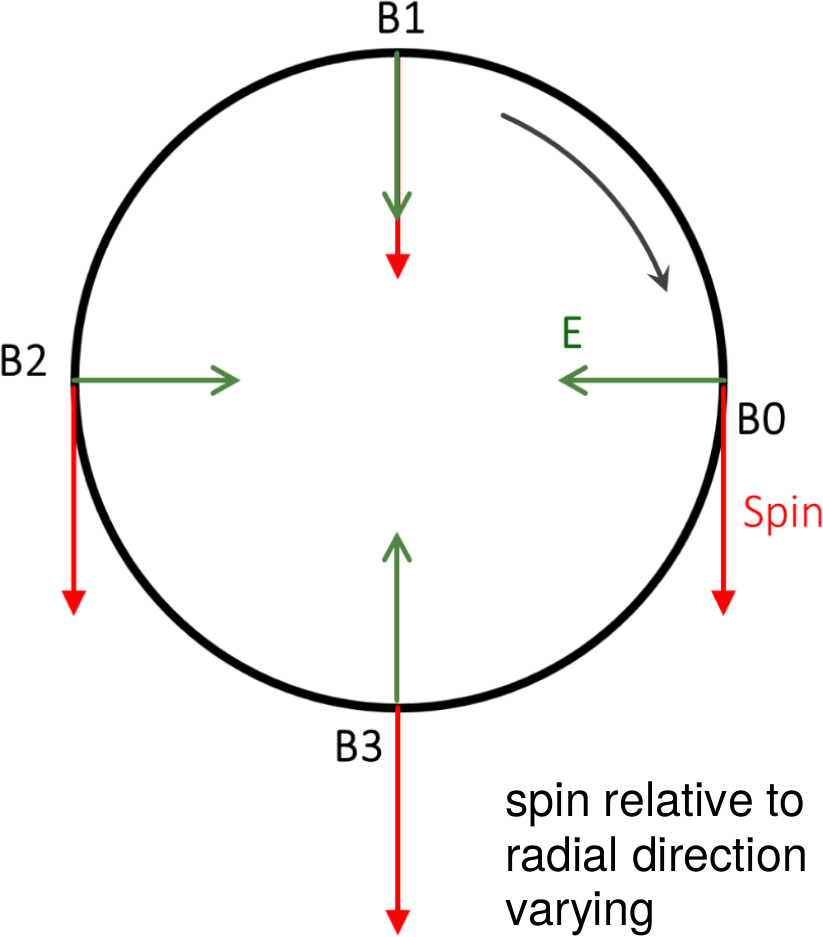
\includegraphics[height=0.4\textheight]{phases-and-bunches.png} 
		\caption{$\phi_a$ not known $\rightarrow$ use perpendicular beam polarization with 4 bunches}
	\end{figure}
	\vspace{-0.6cm}
	
		\column{0.45\textwidth}
		\vspace{-0.3cm}
		\begin{figure}
			\centering
			\vspace{-0.1cm}
			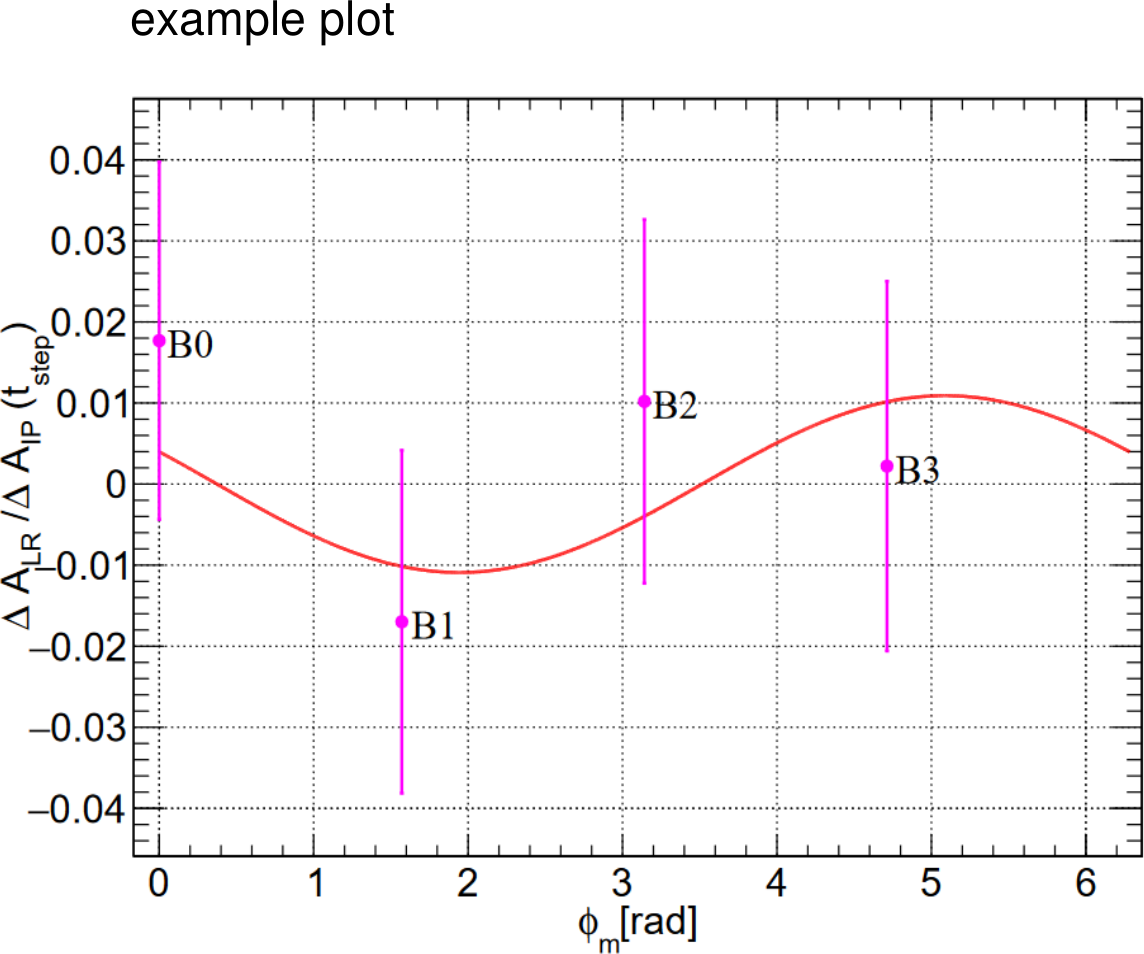
\includegraphics[height=0.4\textheight]{fit-sinus-oscillation-to-pol-jump.png}
			\caption{Left-Right asymmetry for one cycle and four bunches simultaneously orbiting.}
		\end{figure}
	\vspace{-0.6cm}

	\end{columns}
\end{block}

\end{frame}

\begin{frame}
\frametitle{Bound on oscillating EDM of deuteron\,\textcolor{PineGreen}{\cite{PhysRevX.13.031004}}}


\centering
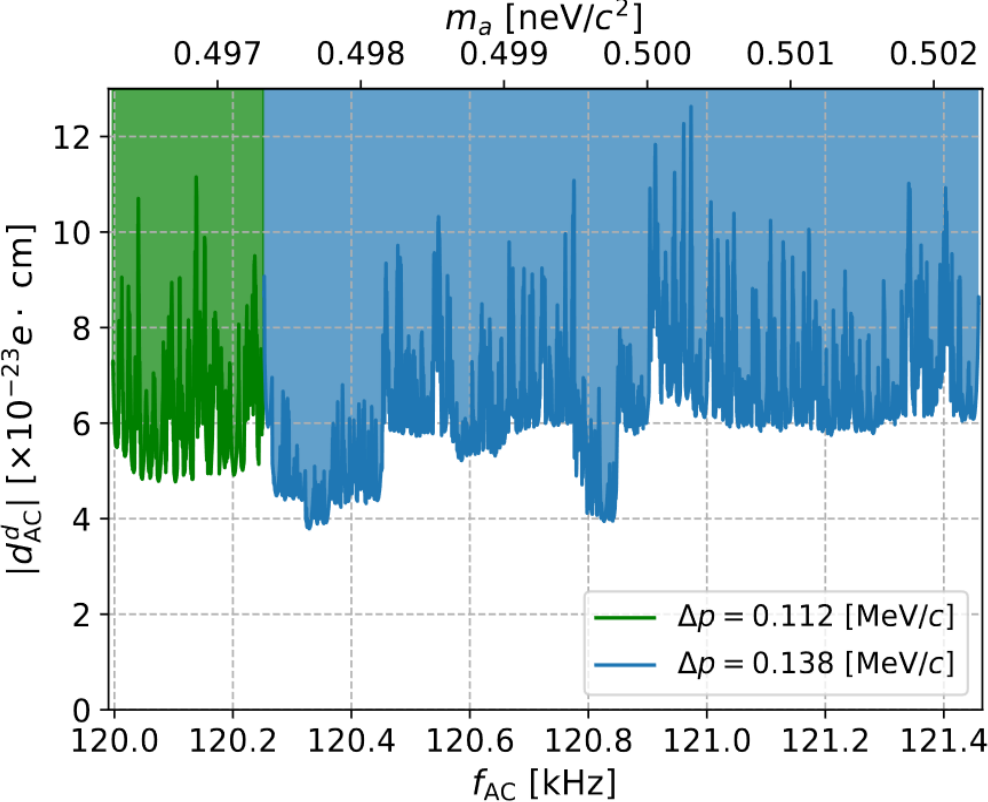
\includegraphics[width=0.6\textwidth]{oscillating-EDM-limits.png}

\vspace{-0.2cm}
\begin{alertblock}{Observed oscillation amplitudes from 4 bunches}
\begin{itemize}
	\item 90\% CL upper limit on the ALPs induced oscillating EDM
	\item Average of individual measured points
	$d_\text{AC} < \SI{6.4e-23}{e.cm}$	
\end{itemize}

\end{alertblock}
\end{frame}
\begin{frame}
\frametitle{Bound on ALP-EDM coupling}

\centering
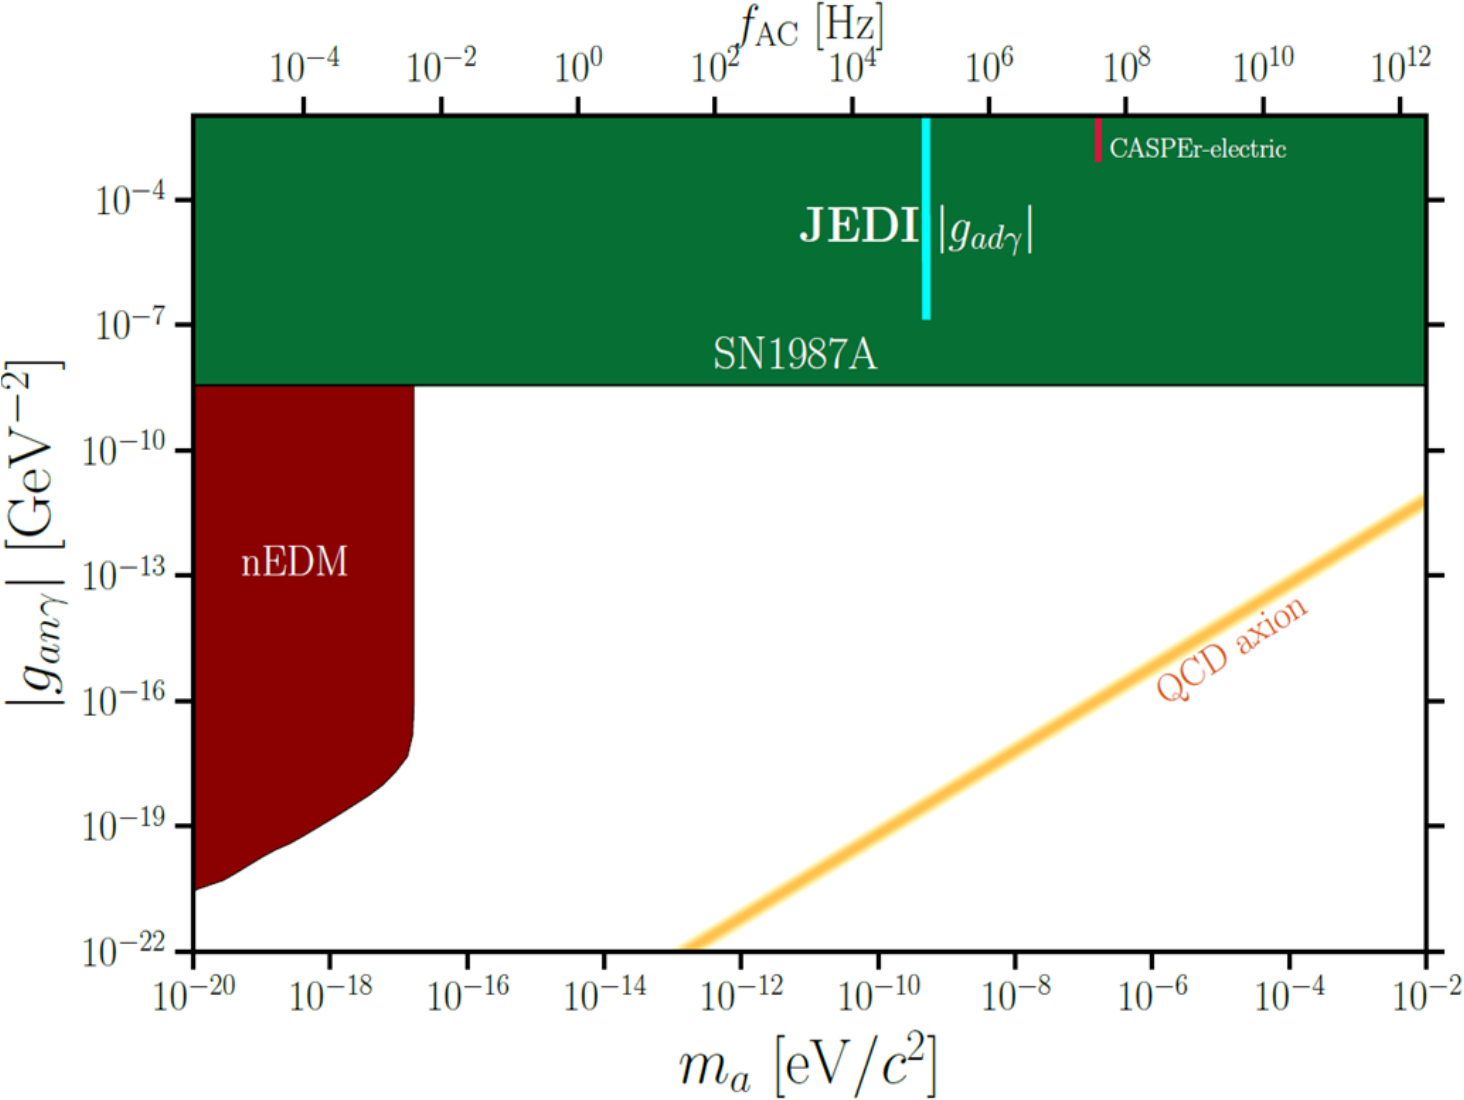
\includegraphics[width=0.65\textwidth]{ALP-EDM-coupling.png}

\begin{block}{Coupling of ALP to deuteron EDM}
\begin{itemize}
	\item Obtained limit of $g_{ad\gamma} < \SI{1.7e-7}{GeV\squared}$ during few days of data taking.
	\item For further details and various ALP couplings, see\,\textcolor{PineGreen}{\small \cite{PhysRevX.13.031004}}.
\end{itemize} 
 
	
\end{block}
\end{frame}
\begin{frame}
\frametitle{ALP-gluon and ALP-nucleon coupling\footnote{Figures courtesy of C.\ O’Hare, “cajohare/axionlimits: Axionlimits,” (2020), \textcolor{blue}{\url{https://doi.org/10.5281/zenodo.3932430}}}}

\begin{columns}
	\column{0.48\textwidth}
	\begin{figure}
		\centering
		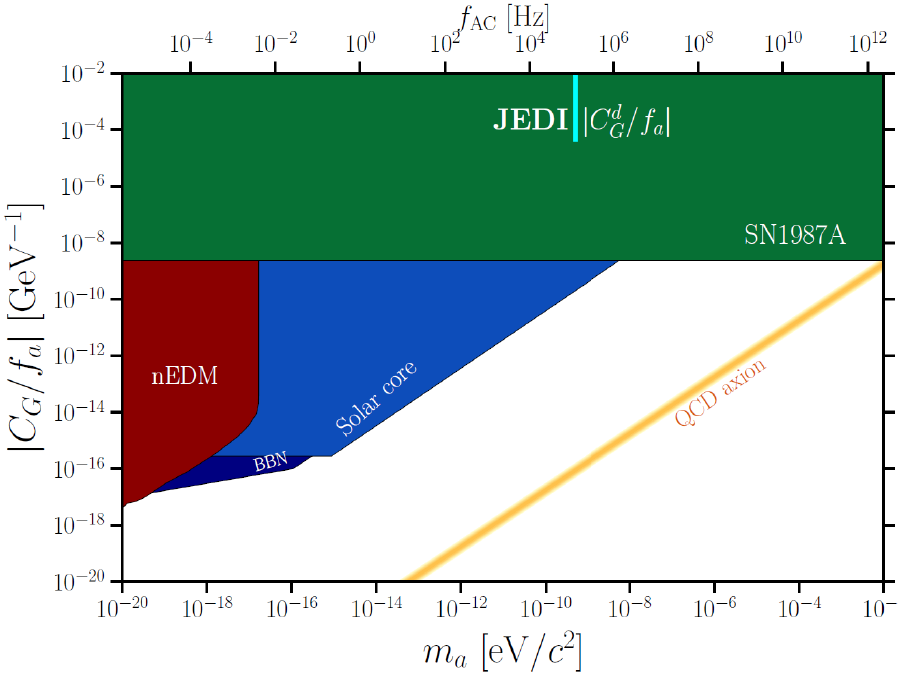
\includegraphics[width=1.\textwidth]{ALP-gluon-coupling.png}
		\caption{ALP-gluon coupling, assuming 100\% oscillating EDM. }
	\end{figure}
	\column{0.48\textwidth}
	\begin{figure}
		\centering
		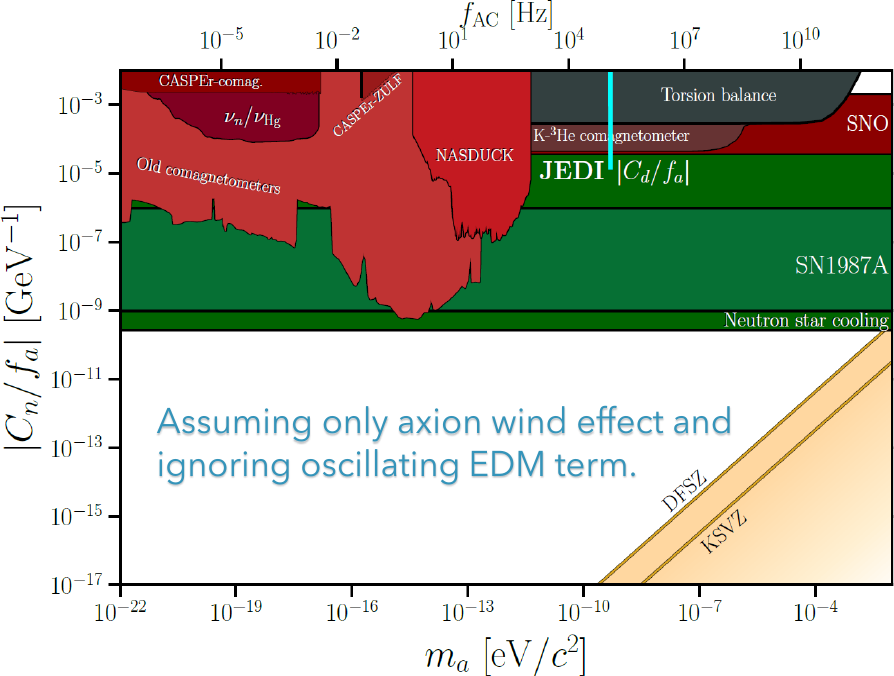
\includegraphics[width=0.98\textwidth]{ALP-nucleon-coupling.png}
		\caption{ALP-nucleon coupling, only axion wind effect, ignoring oscillating EDM term.}
	\end{figure}
\end{columns}

\end{frame}

\section{Staged approach toward dedicated EDM ring }
%--------------------------------------------------------
\begin{frame}
\frametitle{Strategy toward dedicated EDM ring}
%\framesubtitle{ \includegraphics[height = 0.03\textheight]{edm-logo.png} Collaboration: \textcolor{blue}{{\url{http://pbc.web.cern.ch/edm/edm-default.htm}}}}

\vspace{-0.75cm}
\begin{alertblock}{}
	\textbf{Project stages and time frame} \textcolor{PineGreen}{\small \cite[\textcolor{orange}{CYR '21}]{CPEDM:2019nwp}}
\end{alertblock}


\begin{columns}[T]
	\column{0.33\textwidth}
	\hspace{0.2cm}\textbf{Stage 1}
	
	\begin{itemize}
		\item \small \textbf{\textcolor{Maroon}{Precursor experiment}}
	\end{itemize}
	
	\column{0.33\textwidth}
	\hspace{0.2cm}\textbf{Stage 2}
	\begin{itemize}
		\item \small \textbf{\textcolor{Maroon}{Prototype ring}} 
	\end{itemize}
	
	\column{0.33\textwidth}
	\hspace{0.2cm}\textbf{Stage 3}
	\begin{itemize}
		\item \small \textbf{\textcolor{Maroon}{Dedicated storage ring}} 
	\end{itemize}
\end{columns}


\begin{columns}
	\column{0.33\textwidth}
	\centering
	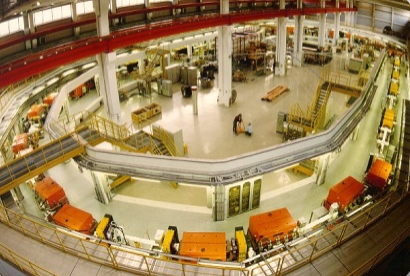
\includegraphics[width=0.6\textwidth]{COSY-foto-2.png}
	
	\column{0.33\textwidth}
	\centering
	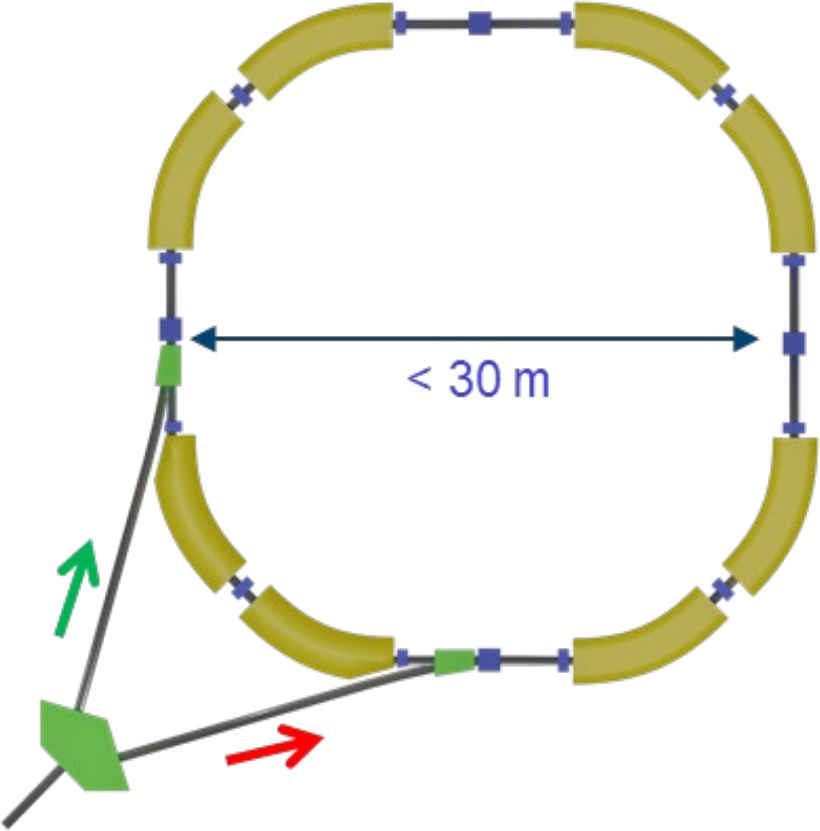
\includegraphics[width=0.6\textwidth]{PSR-topview.png}
	
	\column{0.33\textwidth}
	\centering
	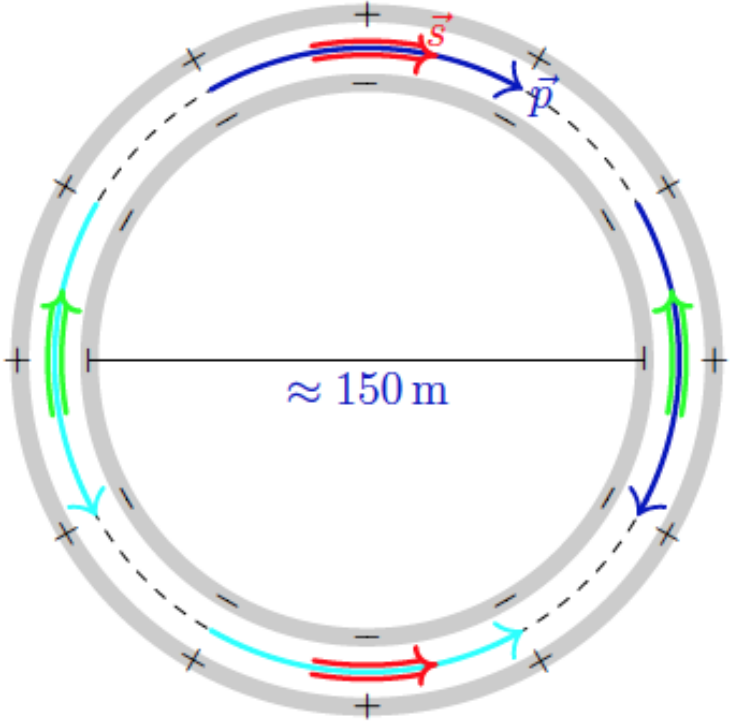
\includegraphics[width=0.6\textwidth]{dedicated-ring.png}
	
\end{columns}

\begin{columns}[T]
	\column{0.35\textwidth}
	
	\begin{itemize}
		\item \small magnetic ring 
		\item \small proof-of-capability
		\item \small \nth{1} dEDM \& \nth{1} axion measurement using ring
		\item \small orbit/polarization control
		\item \textbf{now}
	\end{itemize}
	
	\column{0.34\textwidth}
	\begin{itemize}
		\item \small Key technologies
		\item \small electric/magnetic bends  
		\item \small simultaneous $\circlearrowleft$ and $\circlearrowright$ 
		\item \small first pEDM measurement
		\item \small \textbf{5 years}
	\end{itemize}
	
	\column{0.35\textwidth}
	\begin{itemize}
		\item \small magic $E_m = \SI{232.79}{MeV}$
		\item \small sensitivity goal \SI{e-29}{e.cm}
		\item \small \textbf{10 years}
	\end{itemize}
\end{columns}


\centering
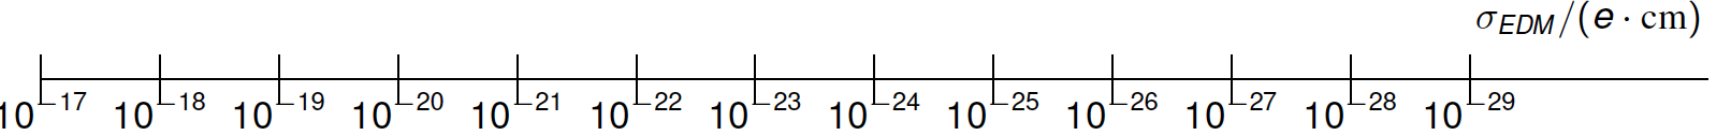
\includegraphics[width=1.0\textwidth]{EDM-scale.png}

\end{frame}
%--------------------------------------------------------
\begin{frame}
\frametitle{\textbf{Stage 2:} Prototype EDM storage ring (PTR)}

\vspace{-0.3cm}
\begin{small}
	\begin{block}{\small \textbf{Build demonstrator for charged-particle EDM}}
			\begin{itemize}
				\item Project prepared by \raisebox{-0.2\height}{
\includegraphics[height=0.4cm]{CPEDM-logo.png}} collaboration (CERN + JEDI + srEDM).
				\item  Physics Beyond Collider process (CERN) \& ESPP Update.
			\end{itemize}
	\end{block}
\end{small}

\vspace{-0.25cm}
\begin{columns}
	\column{0.675\textwidth}
\begin{block}{\small \textbf{100 m circumference}}
	\begin{small}
	\begin{itemize}
		\item $p$ at \SI{30}{MeV} all-electric CW-CCW beams operation
		\item $p$ at \SI{45}{MeV}  frozen spin including additional vertical magnetic fields
	\end{itemize}
	\end{small}
\end{block}

\column{0.25\textwidth}
    \centering
	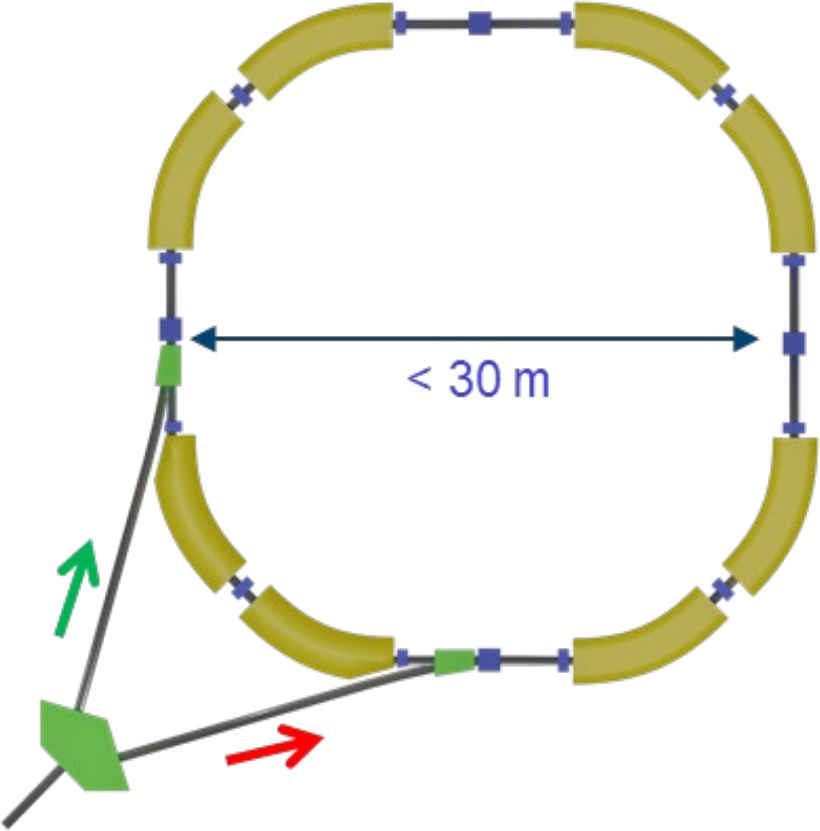
\includegraphics[width=0.55\textwidth]{PSR-topview.png}
\end{columns}

\vspace{-0.1cm}
\begin{block}{\small \textbf{Challenges -- open issues}}
	\begin{small}
	    \begin{multicols}{2}
			\begin{itemize}
				\item All electric \& $E$/$B$ combined bends
				\item Storage time
				\item CW-CCW operation with orbit difference to pm
				\item Spin-coherence time
				\item Polarimetry
				\item Magnetic moment effects (shielding) 
				\item Stochastic cooling
			\end{itemize}
		\end{multicols}
	\end{small}
\end{block}		

\vspace{-0.25cm}
\begin{alertblock}{\small \textbf{Primary purpose of PTR}}
\begin{small}
		\begin{itemize}
		\item \textbf{Study open issues and perform first direct proton EDM measurement}.
	\end{itemize}
\end{small}
\end{alertblock}
\end{frame}
%------------------------------------------------

\section{Summary}

\begin{frame}[t,allowframebreaks]
\frametitle{Summary}
\framesubtitle{}

\begin{exampleblock}{Status of JEDI experiments on EDMs and axions/ALPs}
	\begin{itemize}
		\item \textbf{Results \& achievements} \raisebox{-0.2\height}{
\includegraphics[height=0.4cm]{CPEDM-logo.png}} summarized in  \textcolor{orange}{CERN Yellow Report}\,\textcolor{PineGreen}{\cite{CPEDM:2019nwp}}.
		\item \textbf{Determination of coupling limit ALPs to deuteron EDM} at COSY\,\textcolor{PineGreen}{\cite{PhysRevX.13.031004}}: $$\boxed{g_{ad\gamma} < \SI{1.7e-7}{GeV\squared}}$$
		\vspace{-0.3cm}
		\begin{itemize}
			\item[-] Frequency range: \SI{119997}{Hz} to \SI{121457}{Hz}, total width $\approx \SI{1500}{Hz}$.	
			\item[-] ALP mass range: \SI{0.496}{neV} to \SI{0.502}{neV}.
			\item[-] Potential to enlarge scanned frequency range at expense of lower sensitivity.
			\item[-] High sensitivity for \textit{dedicated} frequency (mass) scans.
			\item[-] Technique can also exploit  sidebands  $\omega_a = \omega_s + k \cdot \omega_\text{rev}$, $k\in \mathbb{Z}$.		
		\end{itemize} 
		\item \textbf{Deuteron EDM measurements at COSY: }
		\begin{itemize}
			\item[-] Good  data from both Precursor I (3 maps with IS method) Precursor II (2 maps IS + 5 maps with pilot bunch)
			\item[-] Data analysis in final stages, EDM results in preparation
			\item[-] Focus on systematic studies $\rightarrow$ understand observed tilts of stable spin axis. 
		\end{itemize}
	\end{itemize}
\end{exampleblock}

\begin{alertblock}{Search for charged hadron particle EDMs ($p$, $d$, light ions) in rings:}
\begin{itemize}
 \item \textbf{New window to disentangle sources of $CP$ violation, and to possibly explain matter-antimatter asymmetry of the Universe}
 \begin{itemize}
 	\item[-] Potential sensitivity to gravitational effects\,\textcolor{PineGreen}{\small \cite{CPEDM:2019nwp,ariesWS:2021}}. 	
 \end{itemize}
\item \textbf{Search for static charged particle EDMs} ($p$, $d$, $^3$He) 
 	\begin{itemize}
 		\item[-] EDMs $\rightarrow$ probes of CP-violating interactions $\rightarrow$ Matter-antimatter asymmetry
 	\end{itemize}
 	\item \textbf{Search for oscillating EDMs}:
 	\begin{itemize}
 		\item[-] Axion coupling to gluons and nucleons
 		\item[-] Dark matter search
 	\end{itemize}
 	\item \textbf{New class of (primarily) electrostatic rings required }
 	\begin{itemize}
 		\item[-] Dedicated (final) ring with anticipated sensitivity of $\leq  \SI{e-29}{e.cm}$
 	\end{itemize}
 	\item \textbf{Next step:} Prototype EDM ring development
 	\begin{itemize}
 		\item[-] Intermediate step between precursor (stage 1) and dedicated ring (stage 3)
		\item[-] Goal: \textbf{Study open issues \& perform first direct pEDM measurement}
		\item[-] Pending \textbf{ERC Advanced Research Grant} application to EU, \textbf{Partners:} INFN, CERN, and Aachen, decision in March/April 2024
%		\item[-] \textbf{Host sites} conceived for dedicated EDM storage ring: CERN or COSY.
 	\end{itemize}	
\end{itemize}
\end{alertblock}


\end{frame}


\begin{frame}
%\frametitle{Closing remark}


\centering Thank you for your attention!


\end{frame}


\section*{References}
 \begin{frame}[t,allowframebreaks]
%\begin{frame}[t]
\frametitle{References}
\setbeamertemplate{bibliography item}[text]
\vspace{-0.4cm}
\begin{scriptsize}
%\begin{footnotesize}
	%\bibliographystyle{JHEP}
	\bibliographystyle{apsrev-title}
	%\bibliography{/home/frank/Dokumente/Documents/LITERATUR/spintunemapping_23.01.2017.bib}
	\bibliography{/Users/frankrathmann/Dokumente/Documents/LITERATUR/spintunemapping_22.04.2020.bib}
%\end{footnotesize}
\end{scriptsize}
\end{frame}


% spare slides

\include{slide-to-spare-slides}

\begin{frame}
\frametitle{Experimental requirements for storage ring EDM searches}
\framesubtitle{}

\vspace{-0.2cm}
\begin{block}{High precision, primarily electric storage ring}
 \begin{itemize}
  \item Crucial role of alignment, stability, field homogeneity, and shielding from perturbing magnetic fields.
  \item High beam intensity: \textcolor{blue}{$N = \num{4e10}$ particles per fill}.
  \item High polarization of stored polarized hadrons: \textcolor{blue}{$P=0.8$}.
  \item Large electric fields: \textcolor{blue}{$E = \SI{10}{MV/m}$}.
  \item Long spin coherence time: \textcolor{blue}{$\tau_\text{SCT} = \SI{1000}{s}$}.
  \item Efficient polarimetry with 
  \begin{itemize}
   \item large analyzing power:  \textcolor{blue}{$A_y \simeq 0.6$},
   \item  and high efficiency detection \textcolor{blue}{$f \simeq 0.005$}.
  \end{itemize}
 \end{itemize}
\end{block}

\vspace{-0.2cm}
\begin{alertblock}{In terms of numbers given above:}
\begin{itemize}
 \item This implies:
 \vspace{-0.3cm}
    \begin{equation}
   \textcolor{blue}{      
   \sigma_\text{stat} = \frac{1}{\sqrt{N \, f} \, \tau_\text{SCT} \, P \, A_y \, E} 
   \quad \Rightarrow \quad \boxed{\sigma_\text{stat}(\SI{1}{yr}) = \SI{e-29}{e.cm}}\,.} 
   \label{eq:statistical-error-EDM-experiment}
    \end{equation}
 \item \textbf{Experimentalist's goal is to provide $\sigma_\text{syst}$ to the same level.}
 \end{itemize}
\end{alertblock}

\end{frame}
\include{slide-new-C-polarimeter}
\include{slide-dC-polarimetry-II}
\begin{frame}
\frametitle{\textbf{Stage 2:} Prototype EDM storage ring (PTR)}

\vspace{-0.3cm}
\begin{small}
	\begin{block}{\small \textbf{Build demonstrator for charged-particle EDM}}
			\begin{itemize}
				\item Project prepared by \raisebox{-0.2\height}{
\includegraphics[height=0.4cm]{CPEDM-logo.png}} collaboration (CERN + JEDI + srEDM).
				\item  Physics Beyond Collider process (CERN) \& ESPP Update.
			\end{itemize}
	\end{block}
\end{small}

\vspace{-0.25cm}
\begin{columns}
	\column{0.675\textwidth}
\begin{block}{\small \textbf{100 m circumference}}
	\begin{small}
	\begin{itemize}
		\item $p$ at \SI{30}{MeV} all-electric CW-CCW beams operation
		\item $p$ at \SI{45}{MeV}  frozen spin including additional vertical magnetic fields
	\end{itemize}
	\end{small}
\end{block}

\column{0.25\textwidth}
    \centering
	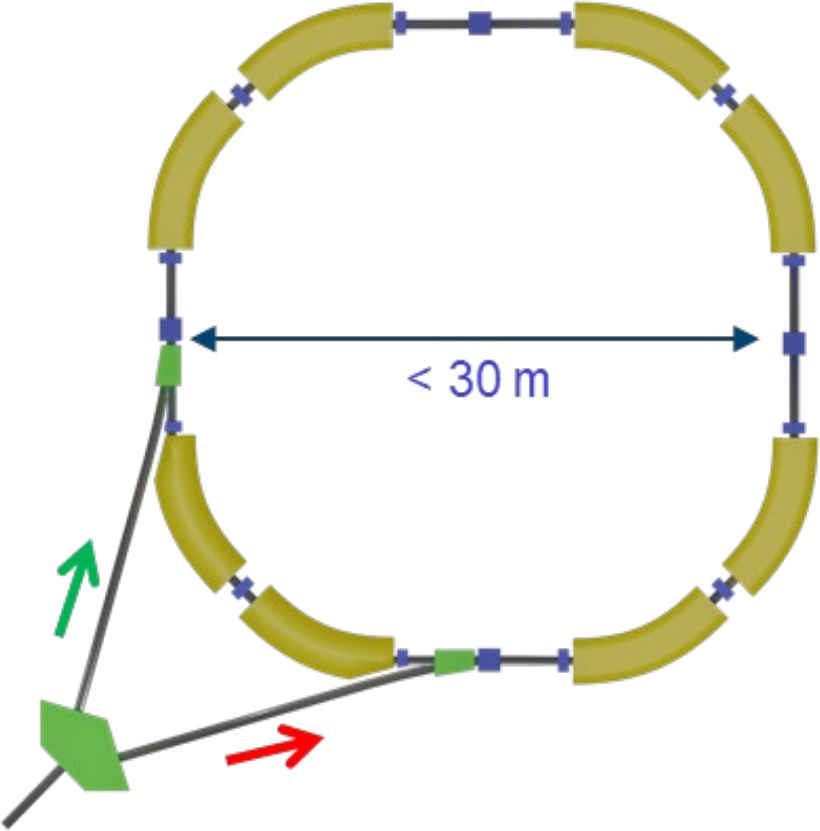
\includegraphics[width=0.55\textwidth]{PSR-topview.png}
\end{columns}

\vspace{-0.1cm}
\begin{block}{\small \textbf{Challenges -- open issues}}
	\begin{small}
	    \begin{multicols}{2}
			\begin{itemize}
				\item All electric \& $E$/$B$ combined bends
				\item Storage time
				\item CW-CCW operation with orbit difference to pm
				\item Spin-coherence time
				\item Polarimetry
				\item Magnetic moment effects (shielding) 
				\item Stochastic cooling
			\end{itemize}
		\end{multicols}
	\end{small}
\end{block}		

\vspace{-0.25cm}
\begin{alertblock}{\small \textbf{Primary purpose of PTR}}
\begin{small}
		\begin{itemize}
		\item \textbf{Study open issues and perform first direct proton EDM measurement}.
	\end{itemize}
\end{small}
\end{alertblock}
\end{frame}
%------------------------------------------------




%-----------------------------------------------------------------------
\end{document}
%-----------------------------------------------------------------------

%\include{slide-EDM-wordlwide-effort}
%\include{slide-status-EDM-searches-table}
%\include{slide-frozen-spin-p-d-3he}

\include{slide-progress-tow-EDM-expts}
\include{slide-COSY-landscape}

\include{slide-spin-tune-tutorial}
\include{slide-principle-polarization-measurement}

\include{slide-principle-polarization-measurement}

\begin{frame}
\frametitle{Detector system: EDDA\,\textcolor{PineGreen}{\cite{Albers:2004iw}}}
\framesubtitle{}
 
 \vspace{-0.6cm}
\begin{columns}[c]
 \column{0.5\textwidth}
 \begin{figure}
     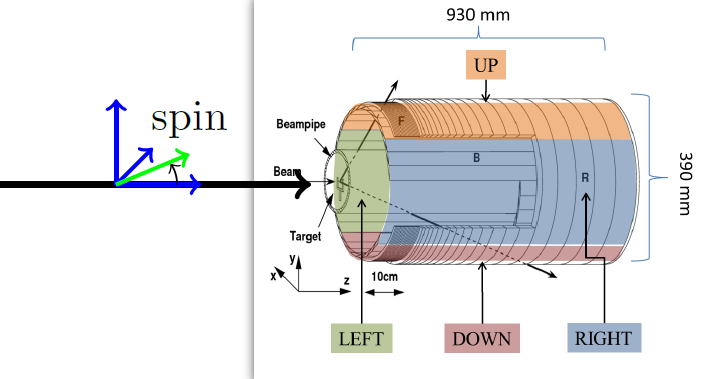
\includegraphics[height=3.5cm]{EDDA.png}
 \end{figure}
 \column{0.35\textwidth}
 \begin{figure}
     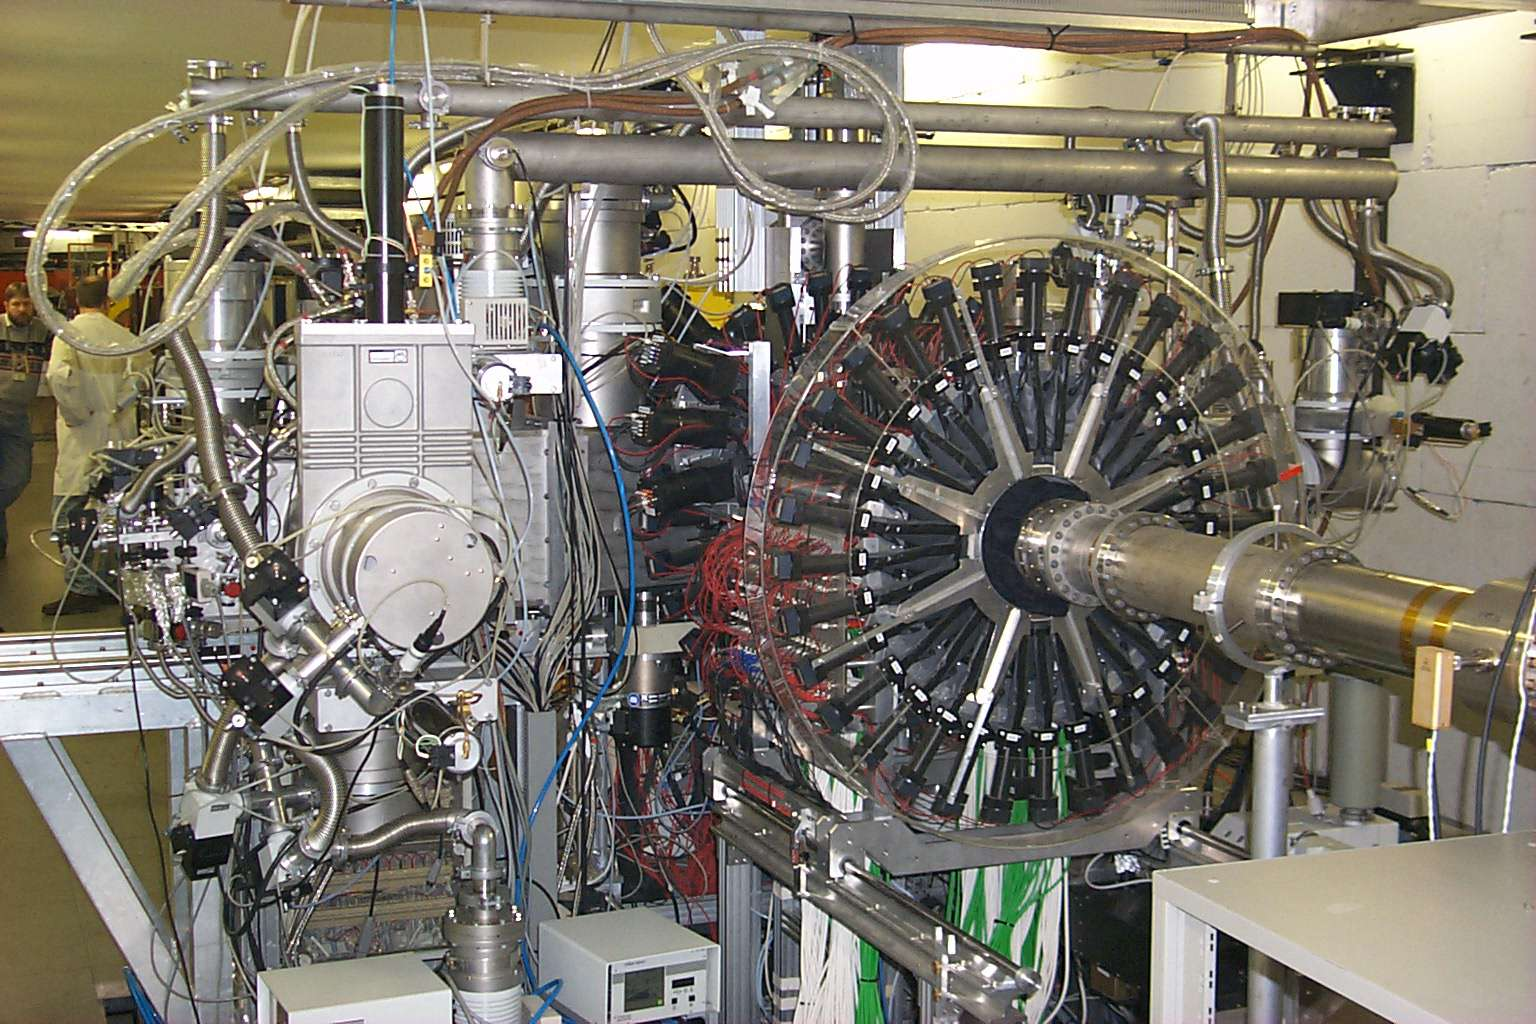
\includegraphics[height=2.5cm]{EDDA-Foto.png} 
 \end{figure}
\end{columns}

\vspace{-0.2cm}
\begin{block}{EDDA  used to determine $\vec p \vec p$ elastic polarization observables:}
\begin{itemize}
 \item Deuterons at $p = \SI{1}{GeV.c^{-1}}$, $\gamma = 1.13$, and $\nu_s = \gamma G \simeq -0.161$
 \item Spin-dependent differential cross section on unpolarized target:
\begin{equation}
    N_\text{U,D} \propto 1 \pm \frac{3}{2} p_x A_y \sin(\underbrace{\nu_s \cdot f_\text{rev}}_{f_s = \SI{-120.7}{kHz}}\cdot t), \text{ where } f_\text{rev} = \SI{750.0}{kHz}.
\end{equation}
\end{itemize}
\end{block}

\vspace{-0.3cm}
\begin{alertblock}{JEPO polarimeter}
	Lateron, EDDA replaced by dedicated new polarimeter, based on LYSO crystals.
\end{alertblock}
 
\end{frame}
\begin{frame}
\frametitle{Spin coherence time}
\framesubtitle{Most polarization experiments unaffected by coherence of spins along $\vec n_\text{co}$}

\vspace{-0.7cm}
\begin{columns}[t]
	\column{0.48\textwidth}
	\begin{exampleblock}{\normalsize \textbf{Spins aligned:}}
		\centering\small Ensemble \textit{coherent}
	\end{exampleblock}
	\vspace{-0.3cm}
	\begin{figure}
		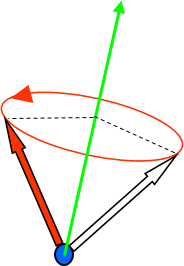
\includegraphics[height=1.5cm]{SCT-1.png}
	\end{figure}
	\column{0.48\textwidth}
	\begin{exampleblock}{\normalsize \textbf{Spin vectors out of phase:} }
		\centering\small Ensemble \textit{decoherent}
	\end{exampleblock}
	\vspace{-0.45cm}
	\begin{figure}
		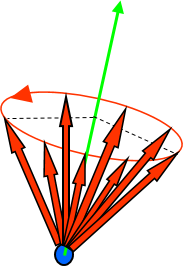
\includegraphics[height=1.5cm]{SCT-2.png}
	\end{figure}
\end{columns}
\begin{center}
	\small  \textbf{$\Rightarrow$ Polarization along $\vec n_\text{co}$ not affected}
\end{center}

\vspace{-0.5cm}
\begin{columns}[]
	\column{0.48\textwidth}
	\begin{exampleblock}{\normalsize \textbf{With frozen spins:} $\vec S \perp  \vec n_\text{co}$:}
		\centering\small Spins aligned
	\end{exampleblock}
	\vspace{-0.3cm}
	\begin{figure}
		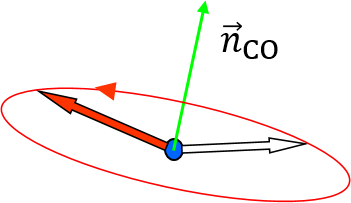
\includegraphics[height=1.1cm]{SCT-3.png}
	\end{figure}
	\column{0.48\textwidth}
	\begin{exampleblock}{\normalsize \textbf{With time:}}
		\centering\small Spins out of phase in horizontal plane
	\end{exampleblock}
	\vspace{-0.3cm}
	\begin{figure}
		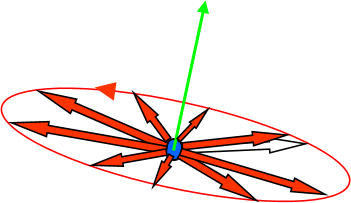
\includegraphics[height=1.1cm]{SCT-4.png}
	\end{figure}
\end{columns}
\begin{center}
	\small  \textbf{$\Rightarrow$ In-plane polarization vanishes}
\end{center}

\vspace{-0.5cm}
\begin{alertblock}{In machines with frozen spins:}
	\centering\textbf{ Buildup time $t$ to observe polarization $p_y(t)$ is limited by $\tau_\text{SCT}$.}
\end{alertblock}

\end{frame}
\begin{frame}
\frametitle{Optimization of spin-coherence time \textcolor{PineGreen}{\cite{PhysRevLett.117.054801}}}
\framesubtitle{}

Precise adjustments of three sextupole families in the ring

\begin{columns}[]
	\column{0.53\textwidth}
	\begin{figure}
		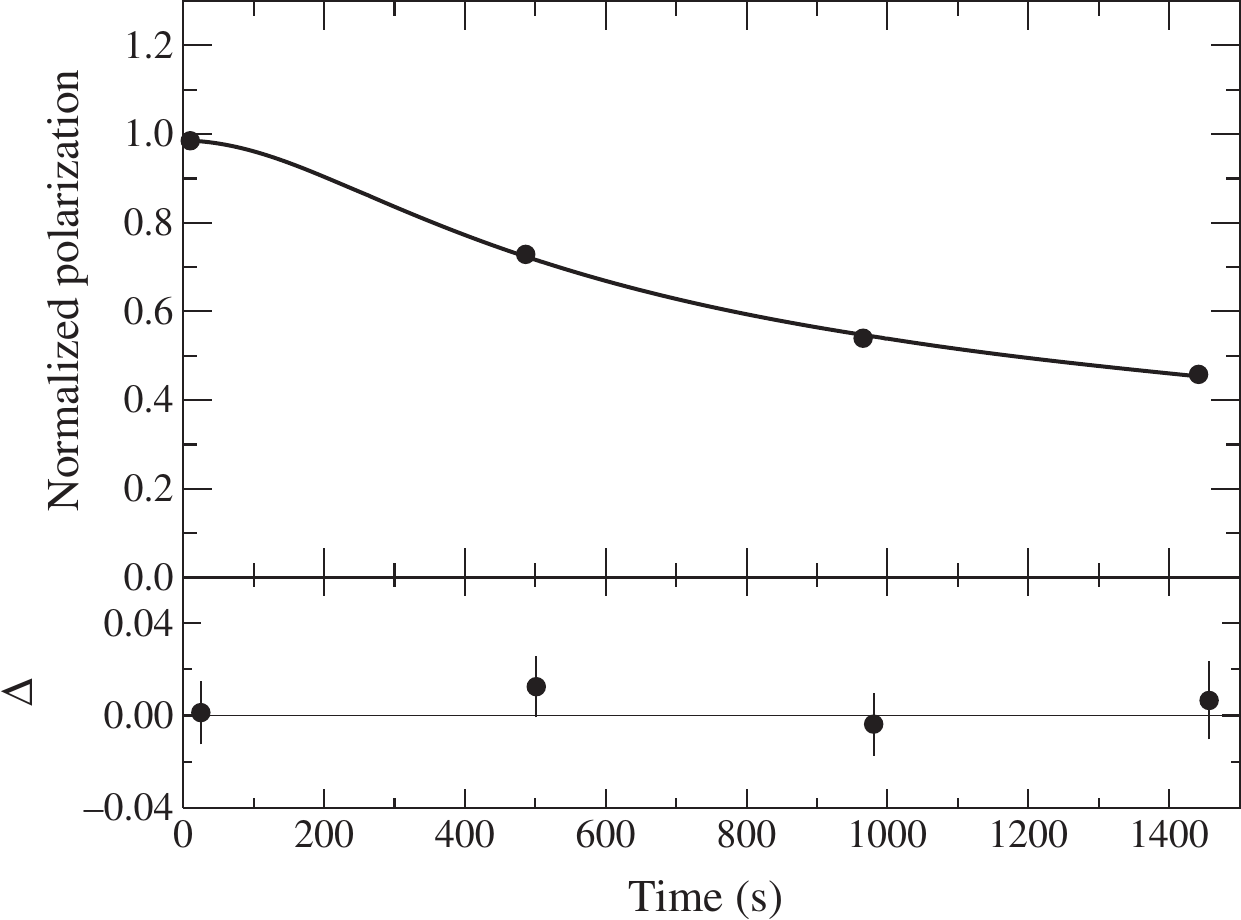
\includegraphics[width=0.95\textwidth]{spin-coherence-time-from-PRL.png}
	\end{figure}
	\column{0.4\textwidth}
	\begin{block}{JEDI progress on $\tau_\text{SCT}$:}
		\begin{equation}
		\textcolor{red}{\mathbf{\tau_\text{SCT} = (782 \pm 117)\,\text{s}}} \nonumber
		\end{equation}
		\vspace{-0.5cm}
		\begin{itemize}
			\item Previous record: $\tau_\text{SCT}(\text{VEPP}) \approx \SI{0.5}{s}$\,\textcolor{PineGreen}{\cite{Vasserman1987302}} ($\approx \num{e7}$ spin revolutions).
		\end{itemize}
	\end{block}
\end{columns}

\begin{alertblock}{\textbf{Spring 2015:} Way beyond anybody’s expectation:}
	\begin{itemize}
		\item With about $\num{e9}$ stored deuterons.
		\item Long spin coherence time was one of main obstacles of srEDM experiments.
		\item Large value of $\tau_\text{SCT}$ of crucial importance (\ref{eq:statistical-error-EDM-experiment}), since $ \sigma_\text{stat} \propto {\tau_\text{SCT}}^{-1}$.
	\end{itemize}
\end{alertblock}

\end{frame}


\begin{frame}
\frametitle{Precision determination of spin tune\,\textcolor{PineGreen}{\cite{PhysRevLett.115.094801}} I}

\begin{block}{Time-stamping events in each detector quadrant accurately:}
\begin{enumerate}
	\item Based on turn number $n$, \SI{100}{s} measurement interval split into turn intervals of $\Delta n = \SI{e6}{turns}$, each interval lasting $\approx \SI{1.3}{\second}$.
	\item  For all events, spin phase advance $\varphi_s = 2 \pi | \nu_s^\text{fix} |n $ calculated assuming certain fixed spin tune $\nu_s^\text{fix}$.
	\item Either map events into one full polarization oscillation in range $\varphi_s \in [0, 2\pi)$, or perform Fourier analysis of rates in detector $\Rightarrow$ determine  $\tilde \varepsilon$ and $\tilde \phi$ in 
	\begin{equation}
	\varepsilon(\varphi_s) = \tilde \varepsilon \sin(\varphi_s + \tilde \varphi)\,.
	\end{equation}
\end{enumerate}
\end{block}

\vspace{0.3cm}
\begin{columns}
	\column{0.45\textwidth}
	\centering 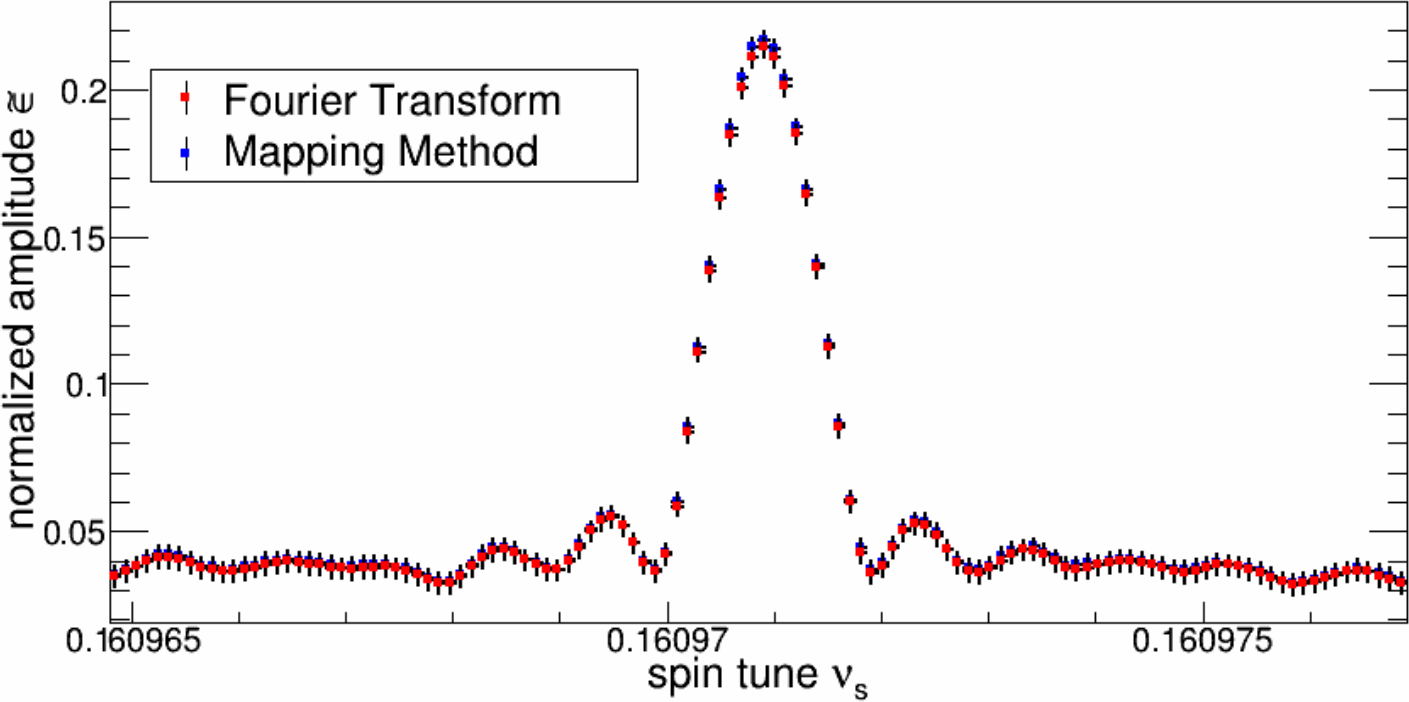
\includegraphics[height = 0.3\textheight]{spin-tune-spectrum.png} 
	\column{0.45\textwidth}  
	\centering 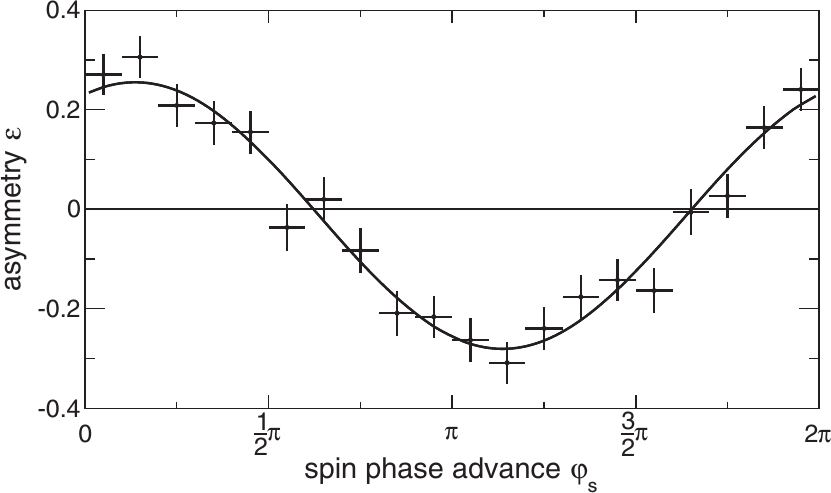
\includegraphics[height = 0.3\textheight]{phase-plot-spin-tune.png}
\end{columns}

\end{frame}
\begin{frame}
\frametitle{Precision determination of the spin tune\,\textcolor{PineGreen}{\cite{PhysRevLett.115.094801}} II}

\vspace{-0.3cm}
\begin{columns}[c]
\column{0.46\textwidth}
\begin{block}{Precise time-stamping of events,}
\begin{itemize}
 \item allows us to monitor phase of measured asymmetry with (assumed) fixed spin tune $\nu_s$ in a $\SI{100}{s}$ cycle:
 \begin{equation}
 \begin{split}
    \nu_s(n) & = \nu_s^\text{fix} + \frac{1}{2\pi} \frac{\dd \tilde{\phi}}{\dd n}\\
             & = \nu_s^\text{fix} + \Delta \nu_s(n)
 \end{split}
 \end{equation}
\end{itemize}
\end{block}

\column{0.5\textwidth}
\begin{figure}
    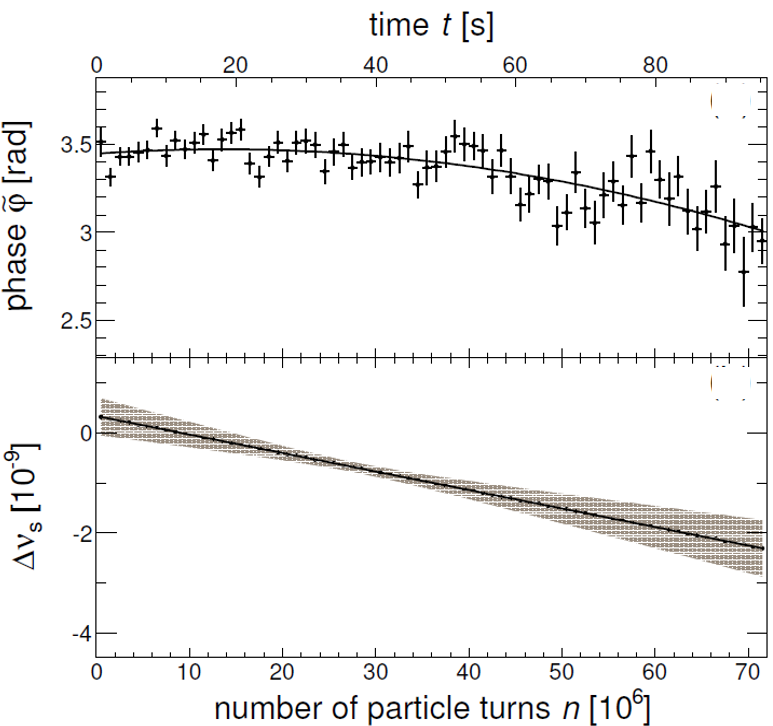
\includegraphics[width=0.9\textwidth]{spin-tune-determination.png}
\end{figure}
\end{columns}

\vspace{-0.2cm}
\begin{alertblock}{Experimental technique allows for:}
\begin{itemize}
 \item Spin tune $\nu_s$ determined to $\approx \num{e-8}$ in $\SI{2}{s}$ time interval.
 \item In a $\SI{100}{s}$ cycle at $t\approx \SI{38}{s}$, interpolated spin tune amounts to
            $|\nu_\text{s}| = (16097540628.3 \pm 9.7)\times 10^{-11}$, \textit{i.e.}, $\Delta \nu_s/\nu_s \approx \num{e-10}$.
 \item \textbf{$\Rightarrow$ new precision tool to study systematic effects in a storage ring.} 
\end{itemize}
\end{alertblock}

\end{frame}

\begin{frame}
\frametitle{Precision determination of the spin tune III}

\begin{columns}

 \column{0.7\textwidth}
 \begin{figure}
    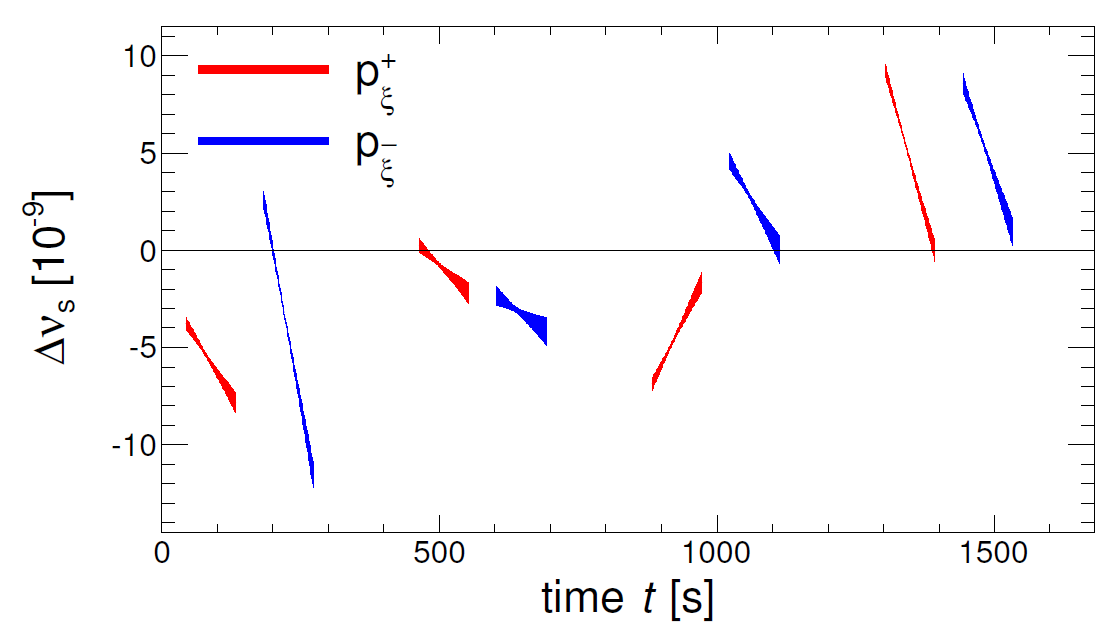
\includegraphics[width=1\textwidth]{spin-tune-walk.png}
 \end{figure}

\column{0.31\textwidth} 
\begin{small}
\begin{block}{}
   Walk of spin tune $\nu_s$ \textcolor{PineGreen}{\cite{PhysRevLett.115.094801}}.
\end{block}
\end{small}
\end{columns}


\begin{alertblock}{Applications of new technique:}
\begin{itemize}
 \item Study long term stability of an accelerator.
 \item Feedback system to stabilize phase of spin precession relative to phase of RF devices ($\rightarrow$  \textit{\textbf{phase-lock}}).
 \item Studies of machine imperfections.
\end{itemize}
\end{alertblock}

\end{frame}


\begin{frame}
\frametitle{Phase locking spin precession in machine to device RF}
 
\vspace{-0.2cm} 
\begin{block}{At COSY, one cannot freeze the spin precession}
 \begin{itemize}
  \item[$\Rightarrow$] To achieve precision for EDM, phase-locking is next best thing to do.
\end{itemize}
\end{block}
 
\vspace{-0.3cm}
\begin{columns}[t]
\column{0.44\textwidth} 
 
\begin{small} 
\vspace{-0.2cm}
\begin{exampleblock}{Feedback system maintains}
	\vspace{-0.2cm}
\begin{enumerate}
 \item resonance frequency, and
 \item phase between spin precession and  device RF (solenoid or WF)
\end{enumerate}
\end{exampleblock}
\end{small}

\vspace{-0.1cm}
\begin{figure}
     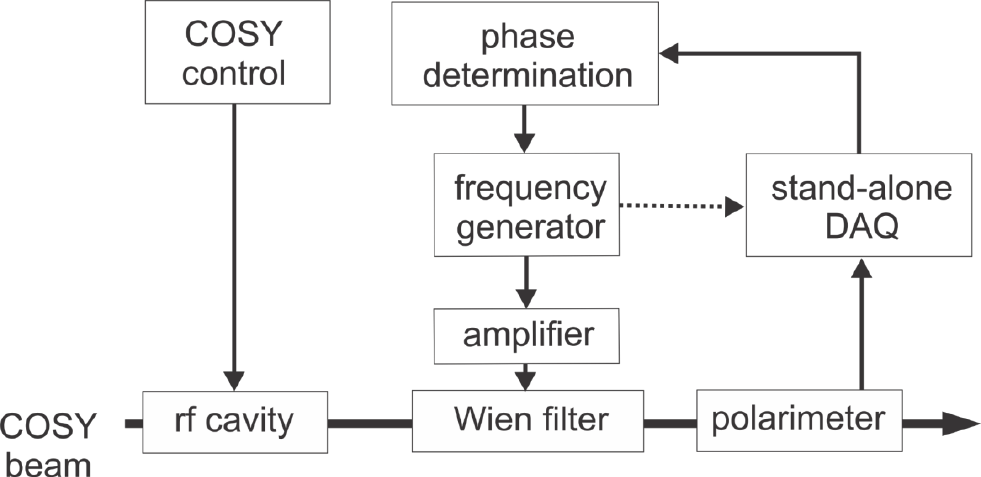
\includegraphics[width = 1\textwidth]{phase-lock-2.png}
\end{figure}

\column{0.5\textwidth} 
\vspace{-0.3cm}
\begin{figure}
     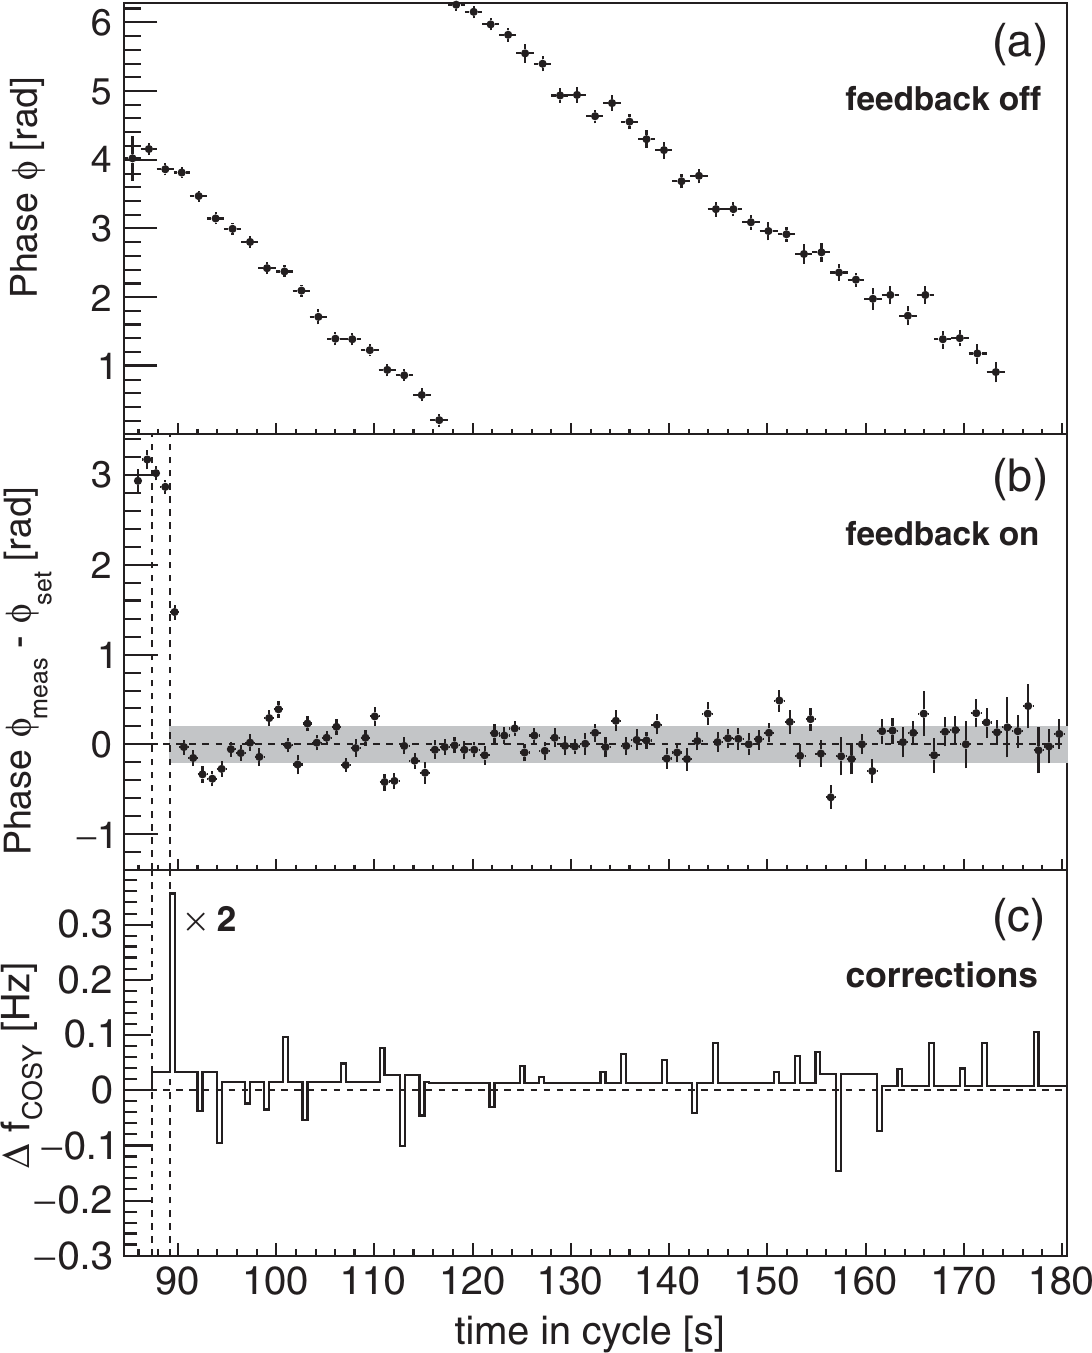
\includegraphics[width = 0.75\textwidth]{phase-locking-fig-1-from-PRL.png}
   \end{figure}
\end{columns}

\vspace{-0.2cm}
\begin{alertblock}{}
 \textbf{Major achievement} : Error of phase-lock $\sigma_\phi = \SI{0.21}{rad}$ \textcolor{PineGreen}{\small \cite{PhysRevLett.119.014801}}.
\end{alertblock}

\end{frame}

\include{slide-first-dEDM-motivation}
\include{slide-dC-polarimetry-I}
\include{slide-new-C-polarimeter}

\include{slide-beam-based-alignment-I}
\include{slide-beam-based-alignment-II}
\include{slide-beam-based-alignment-III}
\include{slide-beam-based-alignment-IV}

\include{slide-more-technical-challenges}
\include{slide-EB-deflector-development-Aachen}
\include{slide-EB-deflector-development-Aachen-results}
\include{slide-deflector-real-size}
\include{slide-deflector-real-size-test}

\include{slide-BPM-conventional-vs-rogowski}
\include{slide-rogowski-assembly-stages}
\include{slide-rogowski-position-at-WF-entrance}

\include{slide-proof-of-principle-expt-COSY}
\include{slide-RF-Wien-filter-method}

\include{slide-EDM-expectation-COSY-ideal}
\include{slide-EDM-expectation-COSY-ideal-II}
\include{slide-Function-describing-surface}
\include{slide-preliminary-results-precursor-I}
\include{slide-JEDI-collaboration}
%\include{slide-Lichtenberg}
\include{slide-magic-rings-2}
\include{slide-SCT-tutorial}
\include{slice-machine-imperfections-study}
\include{slide-Driving-circuit}
\include{slide-RF-WF-fotos}
\include{slide-prec-I-and-prec-II-improvements-2}
\include{slide-RF-WF-frequencies}
\include{PTR-lattice-design}
\include{slide-design-study}
\include{slide-presto-timeline}
\include{slide-plan-B}
\include{Beam-transfer-injection-system}

\include{Electrostatic-deflector}
\include{Magnetic-bends}
\include{Multipole-elements}
\include{slide-vacuum-system}
\include{Stochastic-cooling}
\include{slide-RF-cavity}
\include{Spin-manipulation-tools}
\include{polarimeter}
\include{beam-diagnostics}
\include{slide-RF-WF-internal-structure}
\include{slide-RF-WF-EM-simulations}
\include{slide-Lorentz-force-compensation}
\include{slide-first-EDM-like-signals}

